% 4,6 : Paul
% 7,8 : Jo'
% 9,10,11,13: Anthony

\documentclass{article}

\usepackage{a4}
\usepackage{amsmath}
\usepackage{amsfonts}
\usepackage{amssymb}
\usepackage{float}
\usepackage[utf8]{inputenc}
\usepackage[T1]{fontenc}

\usepackage{framed}

\usepackage{graphicx}
\usepackage{caption}
\usepackage{subcaption}
\usepackage{wrapfig}

\usepackage{geometry}


\usepackage{fullpage,graphicx}
\usepackage{rotating}

\usepackage{multirow}

%\setlength{\hoffset}{-18pt}
\setlength{\oddsidemargin}{0cm}     % Marge gauche sur pages impaires
\setlength{\evensidemargin}{0cm}    % Marge gauche sur pages paires
\setlength{\marginparwidth}{54pt}   % Largeur de note dans la marge
\setlength{\textwidth}{17cm}       % Largeur de la zone de texte (17cm)
\setlength{\marginparsep}{7pt}      % Séparation de la marge
\setlength{\topmargin}{-1cm}         % Pas de marge en haut
\setlength{\headheight}{0cm}       % Haut de page
\setlength{\headsep}{10pt}          % Entre le haut de page et le texte
\setlength{\footskip}{27pt}         % Bas de page + séparation
\setlength{\textheight}{23cm}      % Hauteur de la zone de texte (25cm)

\setlength{\parskip}{1ex}
\setlength{\parindent}{1cm}

%\setlength{\topsep}{500pt}
\setlength{\abovecaptionskip}{0.1cm}
\setlength{\belowcaptionskip}{0.5cm}



\newlength{\leftbarwidth}
\setlength{\leftbarwidth}{3pt}
\newlength{\leftbarsep}
\setlength{\leftbarsep}{10pt}
\newlength{\leftbarmargin}
\setlength{\leftbarmargin}{0pt}
\newlength{\defaultparindent}
\setlength{\defaultparindent}{\parindent}


\renewenvironment{leftbar}{%
    \def\FrameCommand{\hspace{\leftbarmargin} \vrule width \leftbarwidth \relax\hspace{\leftbarsep}}%
    \MakeFramed {\advance \hsize -\width \FrameRestore }%
}{%
    \endMakeFramed
}


%\newenvironment{defx}{\noindent \\ \textbf{Definition:} \vspace{-11pt} \begin{leftbar} \vspace{4pt}}{\end{leftbar}}
%\newenvironment{propx}{\noindent \\ \textbf{Proposition:} \vspace{-11pt} \begin{framed}}{\end{framed}}

\newenvironment{defx}{
\setlength{\leftbarwidth}{3pt} 
\setlength{\leftbarmargin}{-2pt} 
\setlength{\leftbarsep}{10pt} 
\begin{leftbar}}{\end{leftbar}}
\newenvironment{propx}{\begin{framed}}{\end{framed}}

\newenvironment{demox}{\footnotesize \noindent \textit{Demo:}  \vspace{-9pt} 
\setlength{\leftbarwidth}{1pt} 
\setlength{\leftbarmargin}{5pt}
\setlength{\leftbarsep}{3pt} 
\setlength{\parindent}{7pt}

\begin{leftbar}}{\end{leftbar}
\setlength{\parindent}{\defaultparindent}
\normalsize}



\newenvironment{deft}[1]{\noindent \\ \textbf{\textsc{#1}} \vspace{-11pt} \setlength{\leftbarwidth}{3pt} 
\setlength{\leftbarmargin}{-2pt} 
\setlength{\leftbarsep}{10pt} 
\begin{leftbar} \vspace{4pt}}{\end{leftbar}}
\newenvironment{propt}[1]{\noindent \\ \textbf{\textsc{#1}} \vspace{-11pt} \begin{framed}}{ \end{framed}}


\newenvironment{algot}[1]{\noindent \\ \textbf{\textsc{#1}} \par \nobreak \vspace{1pt}\hrule\vspace{0pt} \setlength{\parindent}{0cm} \ttfamily} {\normalfont \setlength{\parindent}{\defaultparindent} \par \nobreak \vspace{4pt}\hrule\vspace{15pt}}

\newenvironment{algox}{\noindent \\  \par \nobreak \vspace{1pt}\hrule\vspace{0pt} \setlength{\parindent}{0cm} \ttfamily} {\normalfont \setlength{\parindent}{\defaultparindent} \par \nobreak \vspace{4pt}\hrule\vspace{15pt}}

%\newenvironment{algot}[1]{\noindent \\ \textbf{\textsc{#1}} \par \nobreak \vspace{1pt}\hrule\vspace{0pt} \setlength{\parindent}{0cm} \ttfamily \begin{tabbing} ~~~~\=~~~~\=~~~~\=~~~~\=~~~~\=~~~~\=~~~~} {\end{tabbing} \normalfont \setlength{\parindent}{\defaultparindent} \par \nobreak \vspace{4pt}\hrule \\}

\newcommand{\comment}[1]{\hfill// #1}

\newcommand{\bbB}{\mathbb{B}}
\newcommand{\bbN}{\mathbb{N}}
\newcommand{\bbZ}{\mathbb{Z}}
\newcommand{\bbR}{\mathbb{R}}

\newcommand{\tb}{.~~~~}

%\newcommand{\exsubpart}[1]{\subsection*{#1)}\\ }
\newcommand{\exsubpart}[1]{\subsection*{#1)} \vspace{-51pt} ~\\}

\newcommand{\info}[1]{\small{\textit{(#1)}}}



\graphicspath{{./Images/}}

\begin{document}

\noindent {\fontsize{20}{20}\selectfont \noindent \textbf{Laboratoire d'électronique~:}}

\noindent {\fontsize{30}{30}\selectfont \noindent \textbf{Initiation à la Haute Fréquence}}

\vspace{5pt}\hrule\vspace{2pt}

\noindent {\Large \textbf{\textsc{Masur} Jonathan}\hfill\textbf{\textsc{Graignic} Anthony}\hfill \textbf{\textsc{Gosselin} Paul}}

\vspace{20pt}







\section{Le filtre LC à deux circuits accordés couplés}

\subsection{Description}

On considère le filtre LC à deux circuits accordés couplés décrits Fig.~\ref{fig:LC2circuits}

\begin{figure}[h!]
	\centering
	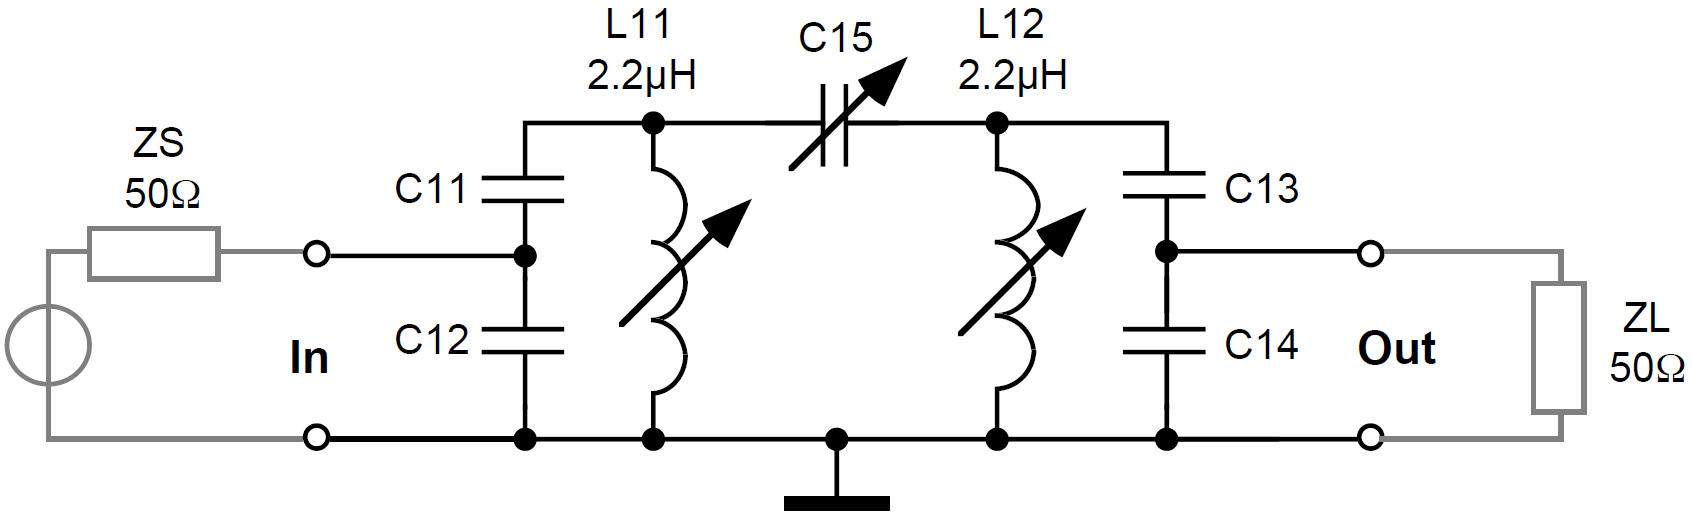
\includegraphics[width=.7\textwidth]{LC2circuits}
	\caption{Filtre LC à deux circuits accordés couplés}
	\label{fig:LC2circuits}
\end{figure}



\subsection{Questions et calculs}


\exsubpart{1}

Ici, on réalise une double adaptation d'impédance, utilisant deux diviseurs capacitifs. Leur concept repose sur l'équivalence décrites Fig.~\ref{fig:capa_divider}.

\begin{figure}[h!]
	\centering
	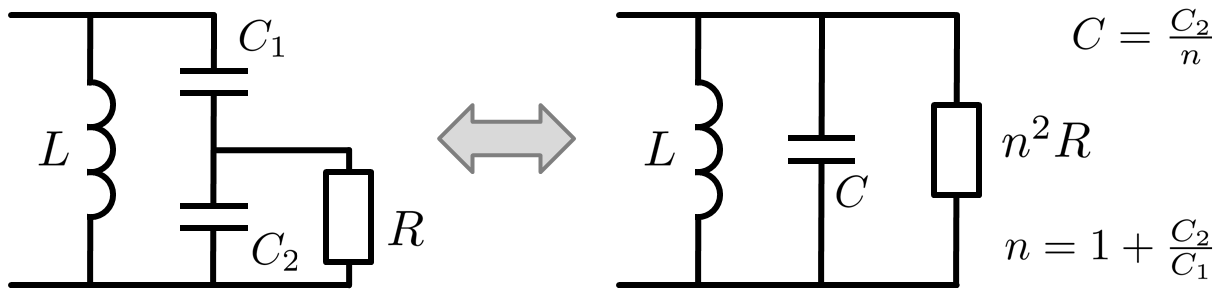
\includegraphics[width=.7\textwidth]{capa_divider}
	\caption{Filtre LC à deux circuits accordés couplés}
	\label{fig:capa_divider}
\end{figure}

Pour juste réaliser l'adaptation d'impédance, il suffirait de mettre uniquement un diviseur capacitif, du côté de l'impédance (de source ou de charge) la plus faible. Toutefois, les condensateurs C11 et C13 ainsi ajoutés permettent d'utiliser en entrée et en sortie du filtre des tensions de valeurs moyennes non nulles. Sans eux, les inductances L11 ou L12 engendreraient un court-circuit vers la masse.

Cela est tout particulièrement intéressant du côté de la source~; et si son impédance est strictement plus faible que l'impédance de charge, l'utilisation d'un unique diviseur capacitif est envisageable. En revanche, si ce n'est pas le cas, deux diviseurs capacitifs seront requis~: le diviseur capacitif placé du côté de la source afin d'en isoler la composante DC augmentera son impédance ressentie, la rendant nécessairement plus élevée que l'impédance de charge, qui devra alors être adaptée.

Évidemment, utiliser en particulier deux diviseurs capacitifs identiques de chaque côté permet de connecter une source et une charge de même impédance, tout en gardant l'avantage susmentionné.


\exsubpart{2}

Une impédance de source ou de charge faussera le diviseur capacitif, résultant d'une part en une désadaptation d'impédance affectant le facteur de qualité du circuit résonnant concerné, d'autre part en une modification de sa fréquence de résonance (modifier $C_2$ dans Fig.~\ref{fig:capa_divider} modifiera $C$). Les effets d'une telle modification de la fréquence de résonance seront évoqués plus bas.


\exsubpart{3}

En augmentant $C_{15}$, on augmente le coefficient de couplage $k$. Si $C_{15}$ est trop faible, le couplage est insuffisant. On parle de sous-couplage~: l'impédance trop élevée crée des pertes. Si $C_{15}$ est trop élevé, les fréquences de résonance des circuits résonnants s'éloignent. On parle de sur-couplage.

Les effets de ces phénomènes sont représentés Fig.~\ref{fig:coupling_effect}

\begin{figure}[h!]
	\centering
	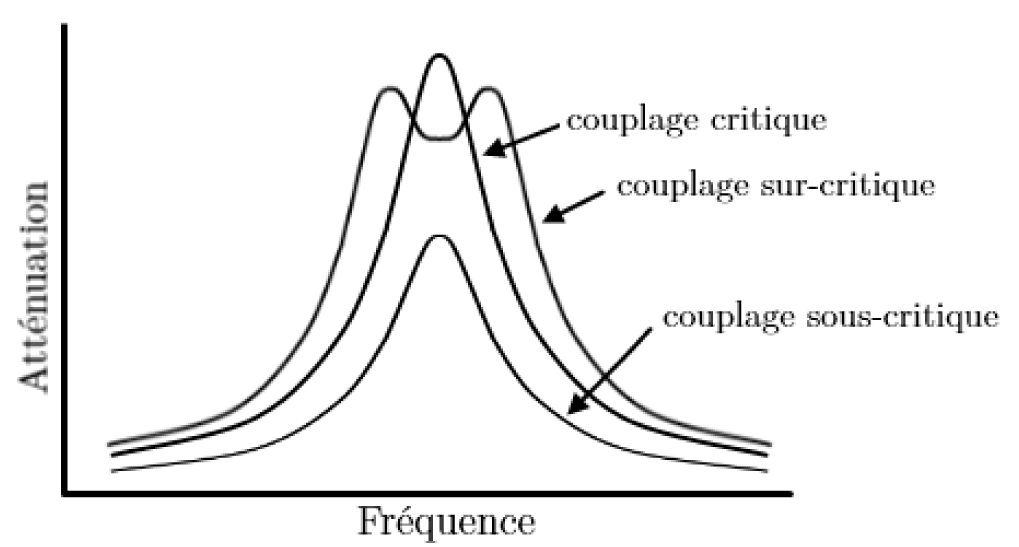
\includegraphics[width=.4\textwidth]{coupling_effect}
	\caption{Effets d'un sous ou sur-couplage}
	\label{fig:coupling_effect}
\end{figure}


\exsubpart{4}

On suppose fixée la résonance désirée $\omega_0$ et les impédances de source et de charge, et on utilise pour chaque circuit résonant les notations de la figure Fig.~\ref{fig:capa_divider}.

Maintenir la résonance ${\omega_0 = \frac{1}{\sqrt{L\cdot C}} = \sqrt{\frac{n}{L\cdot C_2}}}$ impose alors de maintenir~: ${L = \frac{n}{\omega_0^2 C_2} =\frac{C_1+C_2}{\omega_0^2 C_1 C_2}}$.

Le facteur de qualité de chacun des circuits résonants s'écrit~:  valeurs requises pour $L_{11}$ et $L_{12}$ demeurent réalisables avec les inductances variables sélectionnées.


\exsubpart{5}
\begin{equation*}
Q = \omega_0\cdot n^2\cdot R\cdot C = \omega_0\cdot n\cdot R\cdot C_2 = \omega_0\cdot R\cdot C_2\cdot (1+\frac{C_2}{C_1})
\end{equation*}

Ainsi, le facteur de qualité maximal du système sera fixé par les valeurs choisies pour les condensateurs C11, C12, C13, C14. On pourra notamment l'augmenter en augmentant $C_{12}$ et $C_{14}$. Toutefois, il convient de choisir $C_{11}$, $C_{12}$, $C_{13}$, $C_{14}$ de sorte que les

L'équivalence Fig.~\ref{fig:capa_divider} est valable pour des fréquences ${f \gg \frac{1}{2\pi R_S C_{12}}, \frac{1}{2\pi R_L C_{14}}}$. Dans ce domaine de fréquences, le filtre peut être considéré comme un filtre d'ordre 4.

Si l'on considère une plus large gamme de fréquences (des fréquences plus basses), cette équivalence ne peut plus être prise en compte, et l'on observe un filtre d'ordre 6.


\exsubpart{6}

Si l'on considère des fréquences ${f \gg \frac{1}{2\pi R_S C_{12}}, \frac{1}{2\pi R_L C_{14}}}$, après application de l'équivalence Fig.~\ref{fig:capa_divider}, on observe 3 pôles en DC. Ainsi, on aura avant la résonance une pente de la réponse du filtre en amplitude de +60 dB/dec. À noté que si la fréquence de résonance n'est pas suffisamment grande devant ${\frac{1}{2\pi R_S C_{12}}, \frac{1}{2\pi R_L C_{14}}}$, cette pente à +60 dB/dec ne pourra être observée car cachée par la résonance.

Si l'on s'intéresse à de plus basses fréquences (${f \ll \frac{1}{2\pi R_S C_{12}}, \frac{1}{2\pi R_L C_{14}}}$), les diviseurs capacitifs agiront comme passe-bas. On aura aboutira donc pour ces fréquences à une pente +100 dB/dec.

À l'infini, L11 et L12 agissent comme des interrupteurs ouverts tandis que C11, C15, C13 se comportent comme un fil. Les capacités C12 et C14 sont alors placées en parallèle, résultant en un unique pôle à l'infini. Ainsi, on aura après la résonance une pente de la réponse du filtre en amplitude de -20 dB/dec.


\exsubpart{7}

On aurait pu aussi réaliser un couplage capacitif, en remplaçant C15 par une inductance. Cela aurait eu pour avantage de compenser l'effet passe-haut lié aux diviseurs capacitifs, fournissant un filtre plus symétrique sur l'intégralité du spectre~: +60 dB/dec avant la résonance, -60 dB/dec après la résonance si l'on s'intéresse à une très large gamme de fréquence. Dans la gamme de fréquence d'intérêt, on favorise l'atténuation des hautes fréquences~: +20 dB/dec avant la résonance, -60 dB/dec après la résonance. Toutefois, compte tenu de l'utilisation d'une inductance supplémentaire, il s'agit d'une méthode plus coûteuse et moins précise.

On aurait aussi pû réalisé un couplage par transformateur. L'effet sur la réponse en fréquence aurait été le même, mais l'isolation entre la source et la charge s'en serait vue améliorée. Cette méthode plus coûteuse permettrait en revanche de s'affranchir de l'utilisation des inductances L11, L12, remplacées par celles liées au transformateur. Toutefois, le système n'est alors plus réglable. Préserver en parallèle les inductances variables L11, L12 permet de maintenir un réglage manuel, mais ce dernier demeure moins aisé et moins efficace qu'avec un simple couplage capacitif ou inductif.



\exsubpart{8}

??
%TODO


\subsection{Mesures et réglages}

\exsubpart{1}

On prend~: $C_{11}=C_{13}=68\mathrm{pF}$, $C_{12}=C_{14}=390\mathrm{pF}$, $C_{15}^{max}=5\mathrm{pF}$, $L_{11}^{max}=L_{12}^{max}=2,2\mathrm{\mu H}$.

On règle grossièrement les inductances et capacités variables (aboutissant notamment à une légère différence dans les fréquences de résonance). On obtient entre 1MHz et 100MHz les diagrammes de Bode représentés Fig.~\ref{fig:LC2plot}.

\begin{figure}[h]
	\centering
	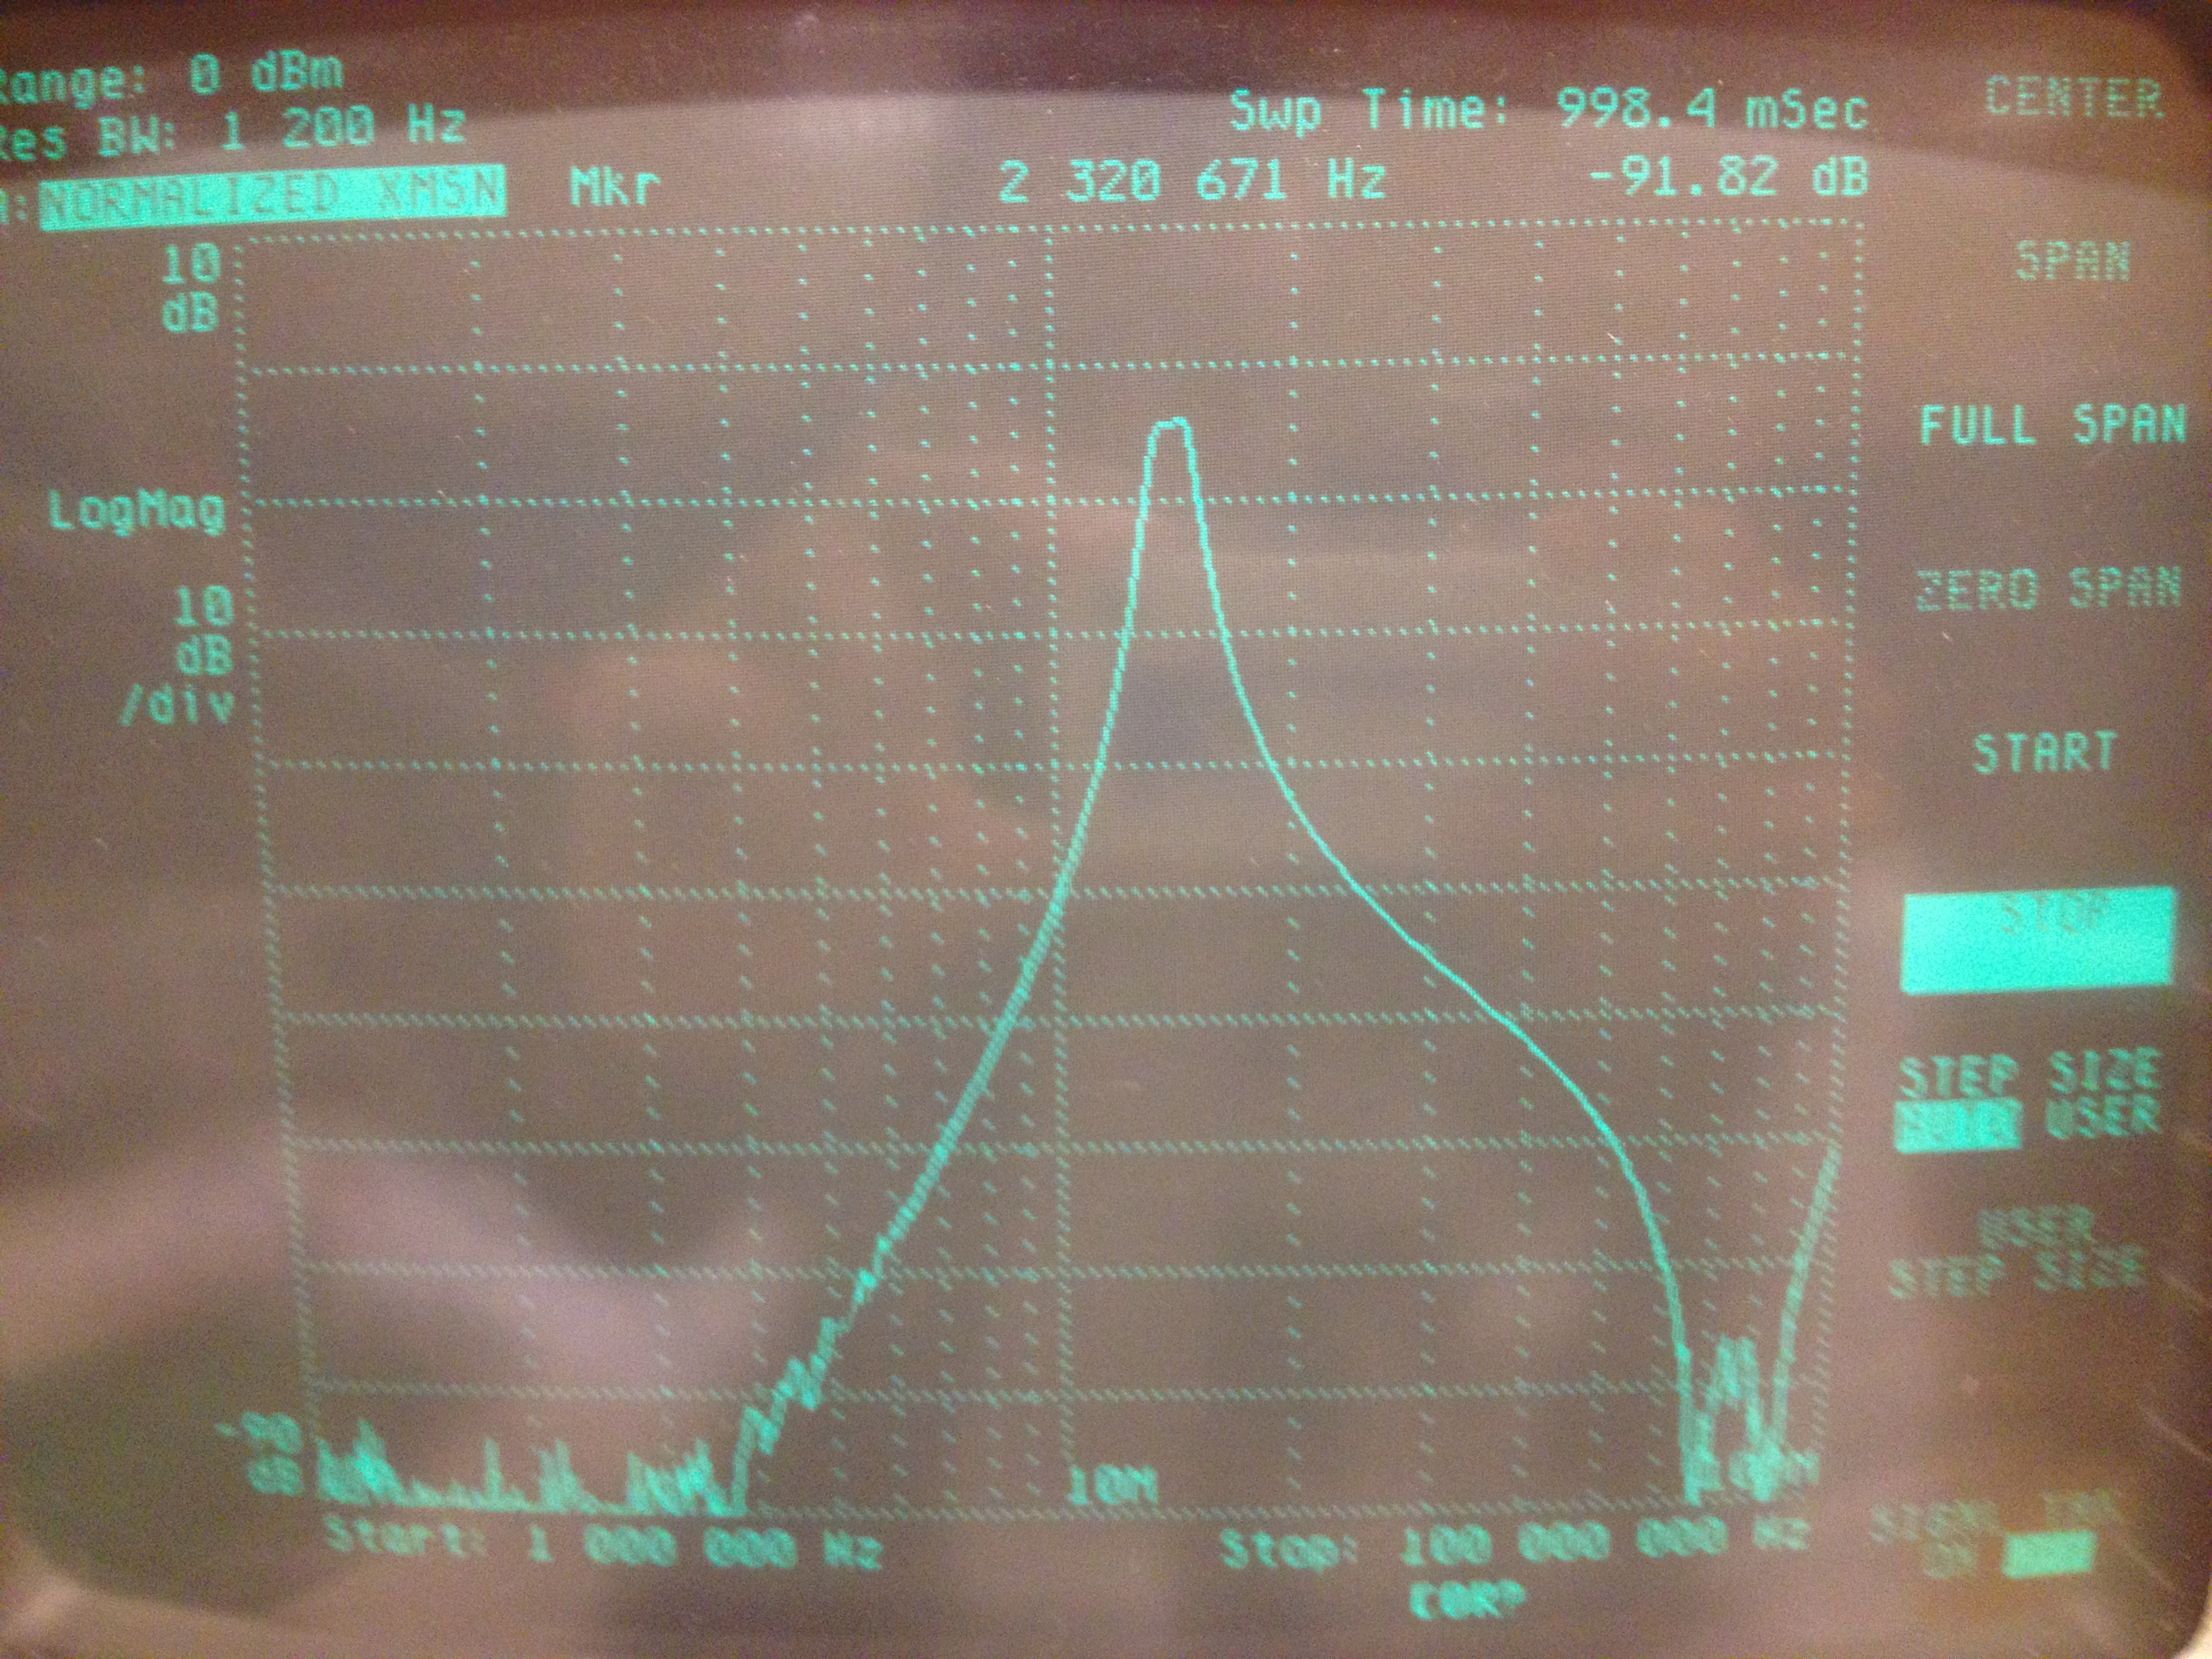
\includegraphics[width=.5\textwidth]{1MHz_100MHz}
	\caption{Diagramme de Bode expérimental pour le filtre LC à deux circuits accordés couplés}
	\label{fig:LC2plot}
\end{figure}

Dans notre cas~: ${\frac{1}{2\pi R_S C_{12}}, \frac{1}{2\pi R_L C_{14}}\approx 8,2\mathrm{MHz}}$. La pente +60 dB/dec, que l'on trouverai entre cette fréquence et la fréquence de résonance, n'est donc pas observable~: elle est effectivement camouflée par la résonance. On observe en revanche bien en deçà de cette fréquence une pente à +100 dB/dec (typiquement autours de 6-7MHz, avant que tracé ne soit perturbé par des bruits divers).

%TODO: Pourquoi -40dB au-dessus ?!


\exsubpart{2,3}

On précise les réglages des inductances et capacités variables. Après avoir réglé L11, L12 de sorte à obtenir des fréquences de résonance identiques, on règle le couplage avec C15. On peut ainsi observé les effets d'un sur-couplage ou d'un sous-couplage comme présenté Fig.~\ref{fig:sur_sous_couple}.

\begin{figure}[h]
	\centering
	\begin{subfigure}[b]{0.43\textwidth}
		\centering
		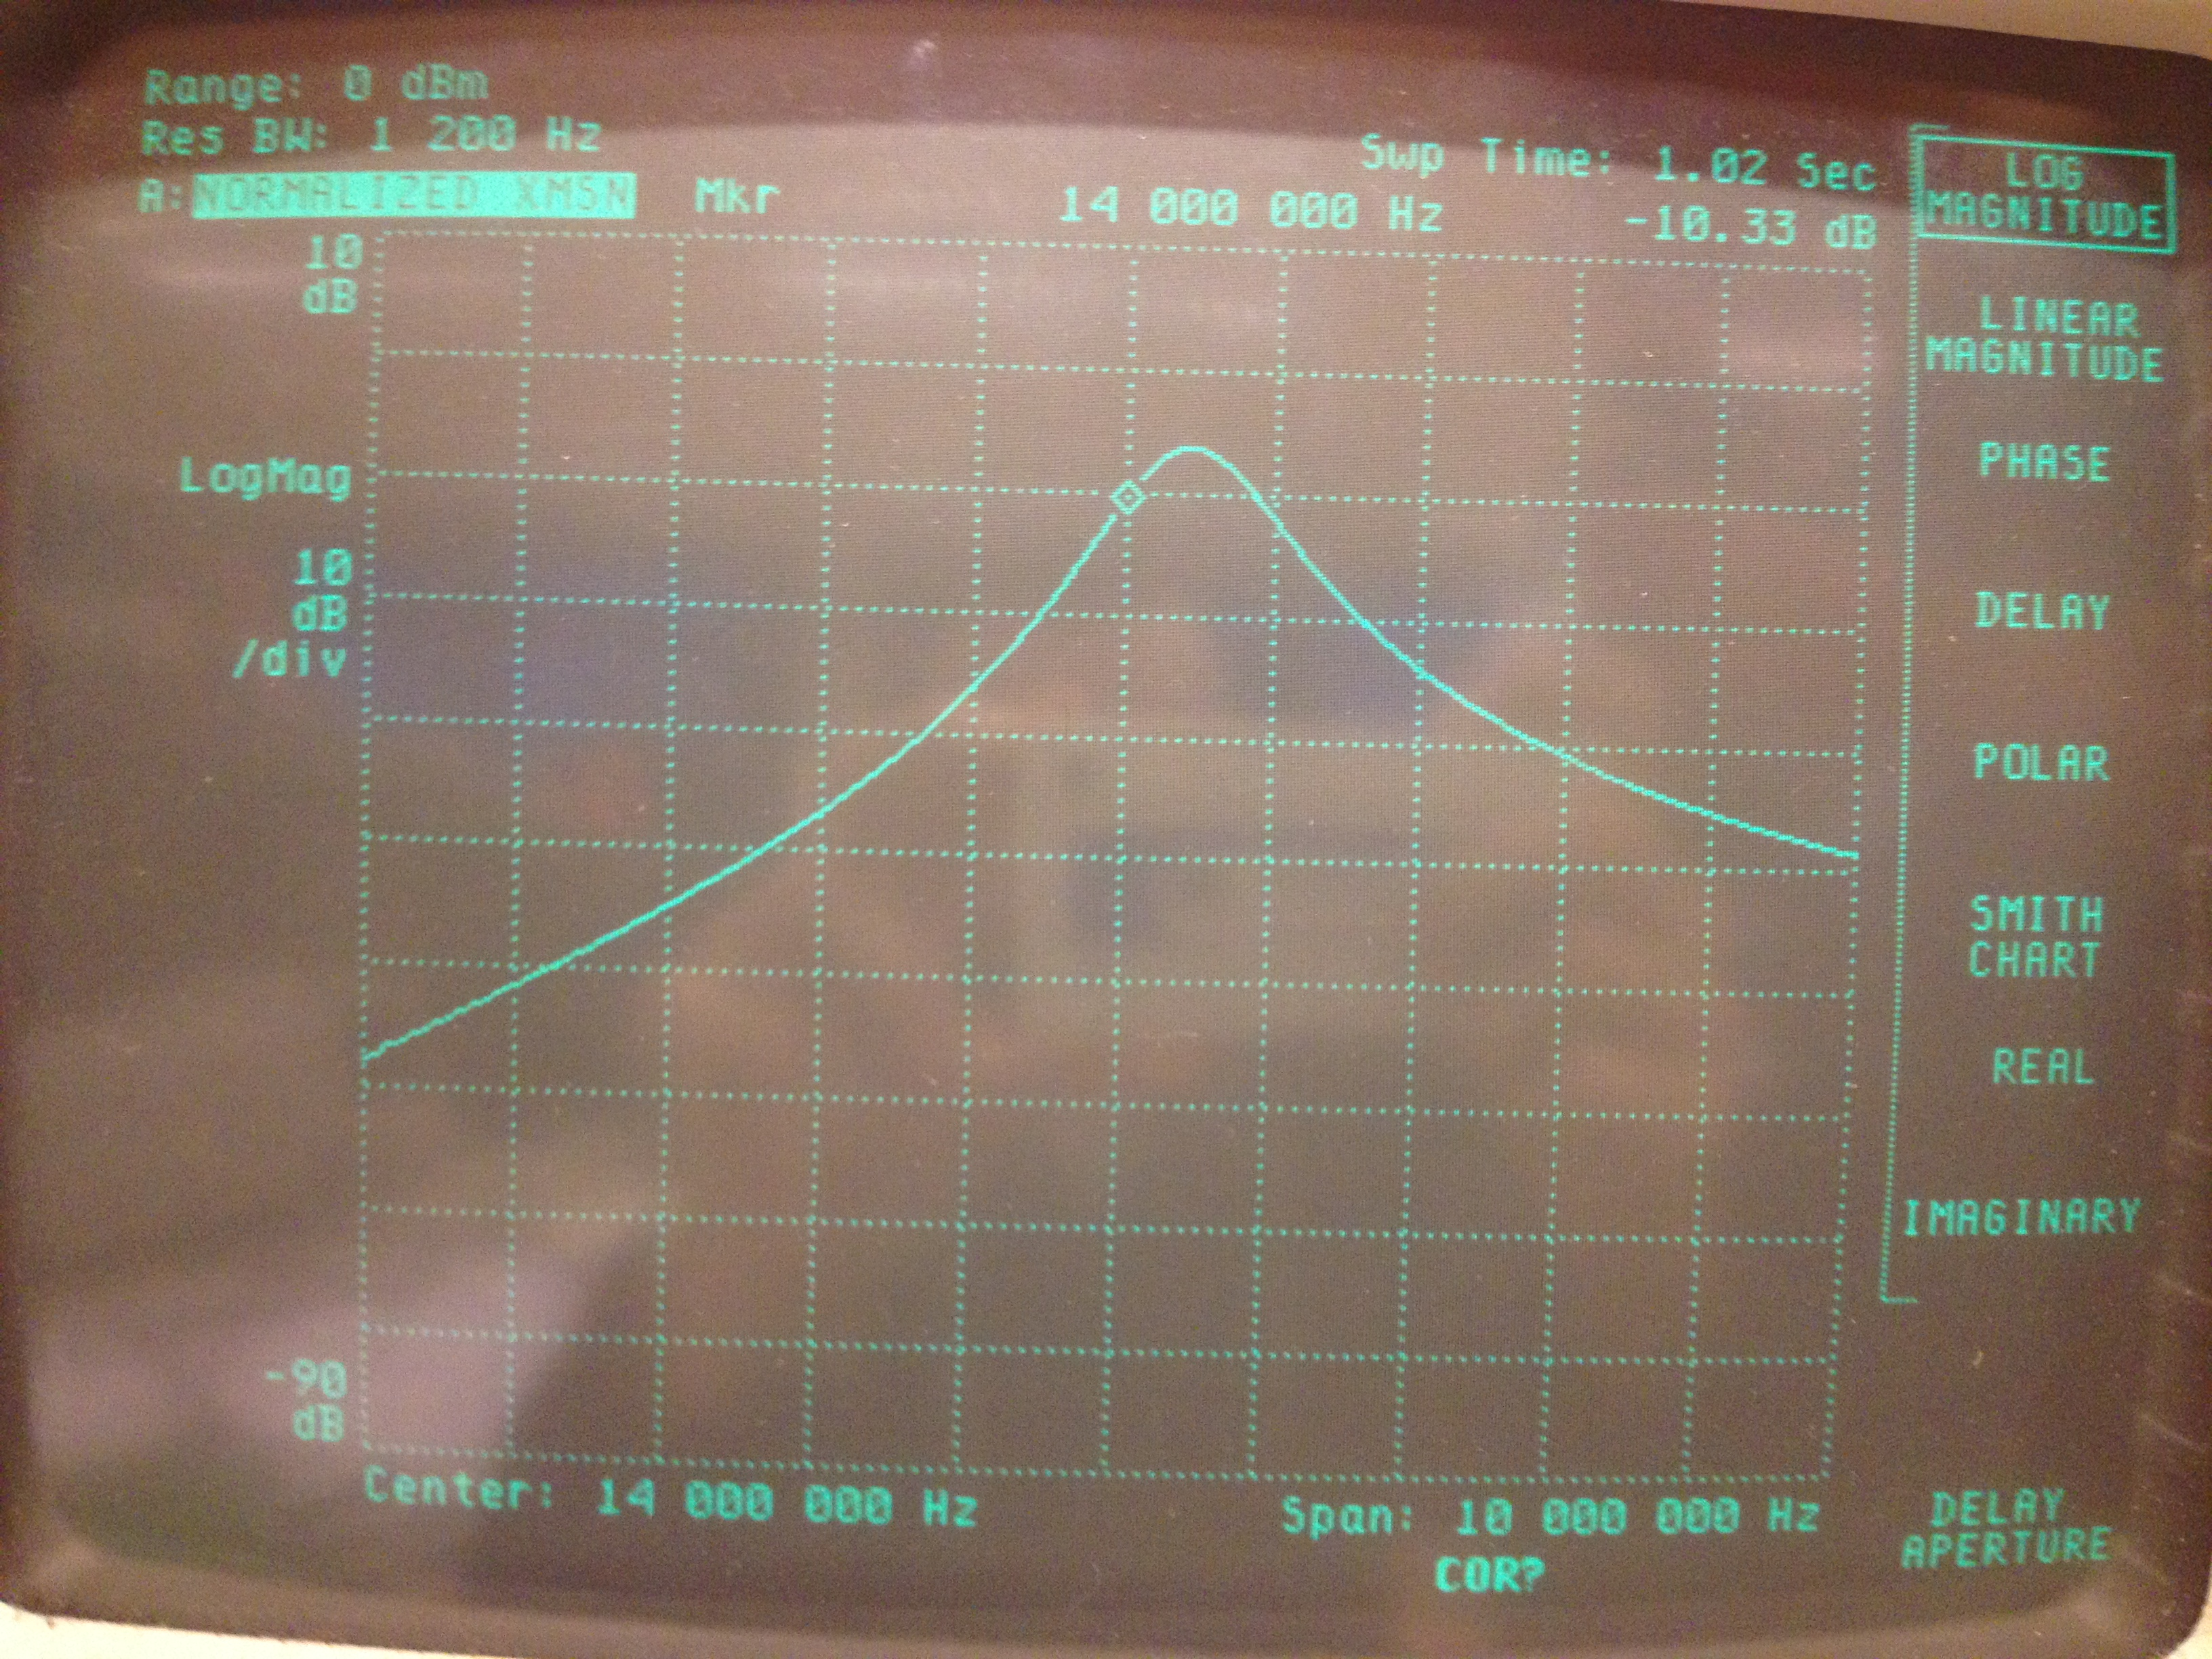
\includegraphics[width=\textwidth]{souscouple}
		\caption{Sous-couplage}
	\end{subfigure}
	\hfill
	\begin{subfigure}[b]{0.43\textwidth}
		\centering
		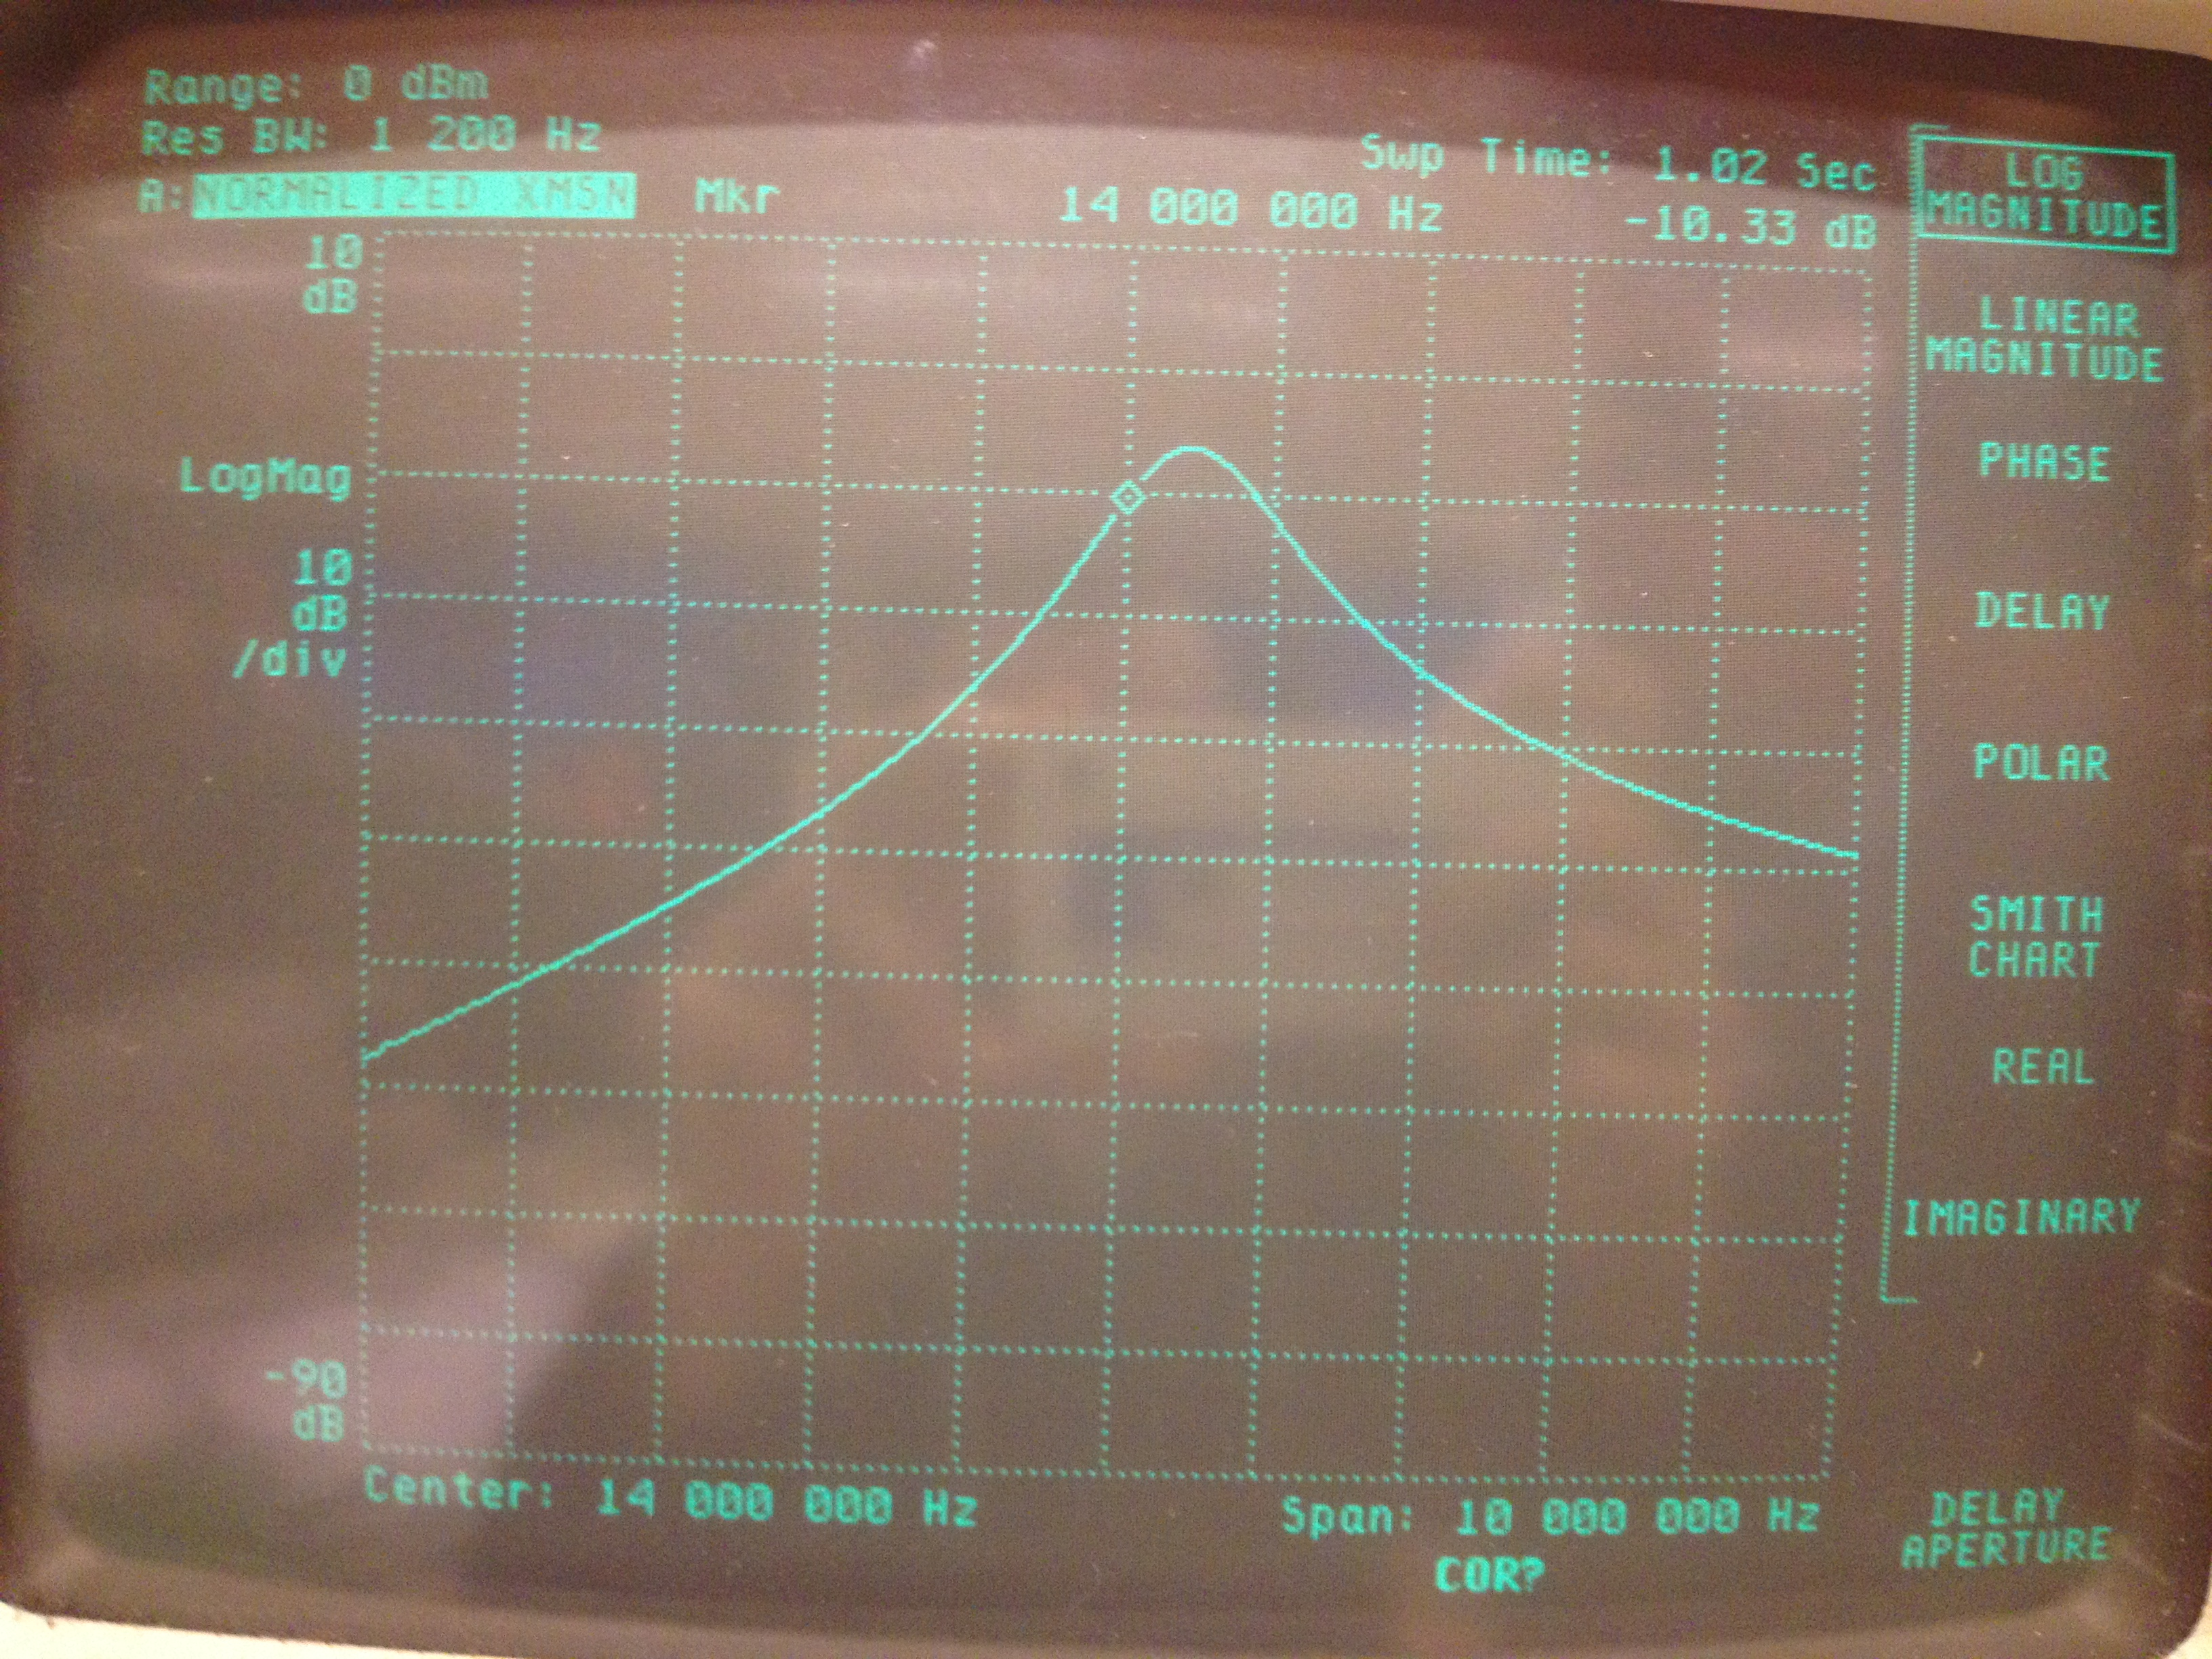
\includegraphics[width=\textwidth]{surcouple}
		\caption{Sur-couplage}
	\end{subfigure}
	\caption{Exemple de sous et sur-couplage}
	\label{fig:sur_sous_couple}
\end{figure}

En effectuant un léger sur-couplage, on obtient les caractéristiques requises~: une bande passante de 2MHz autours 14MHz. Les résultats sont montrés Fig.~\ref{fig:LCregle}.

\begin{figure}[h]
	\centering
	\begin{subfigure}[b]{0.43\textwidth}
		\centering
		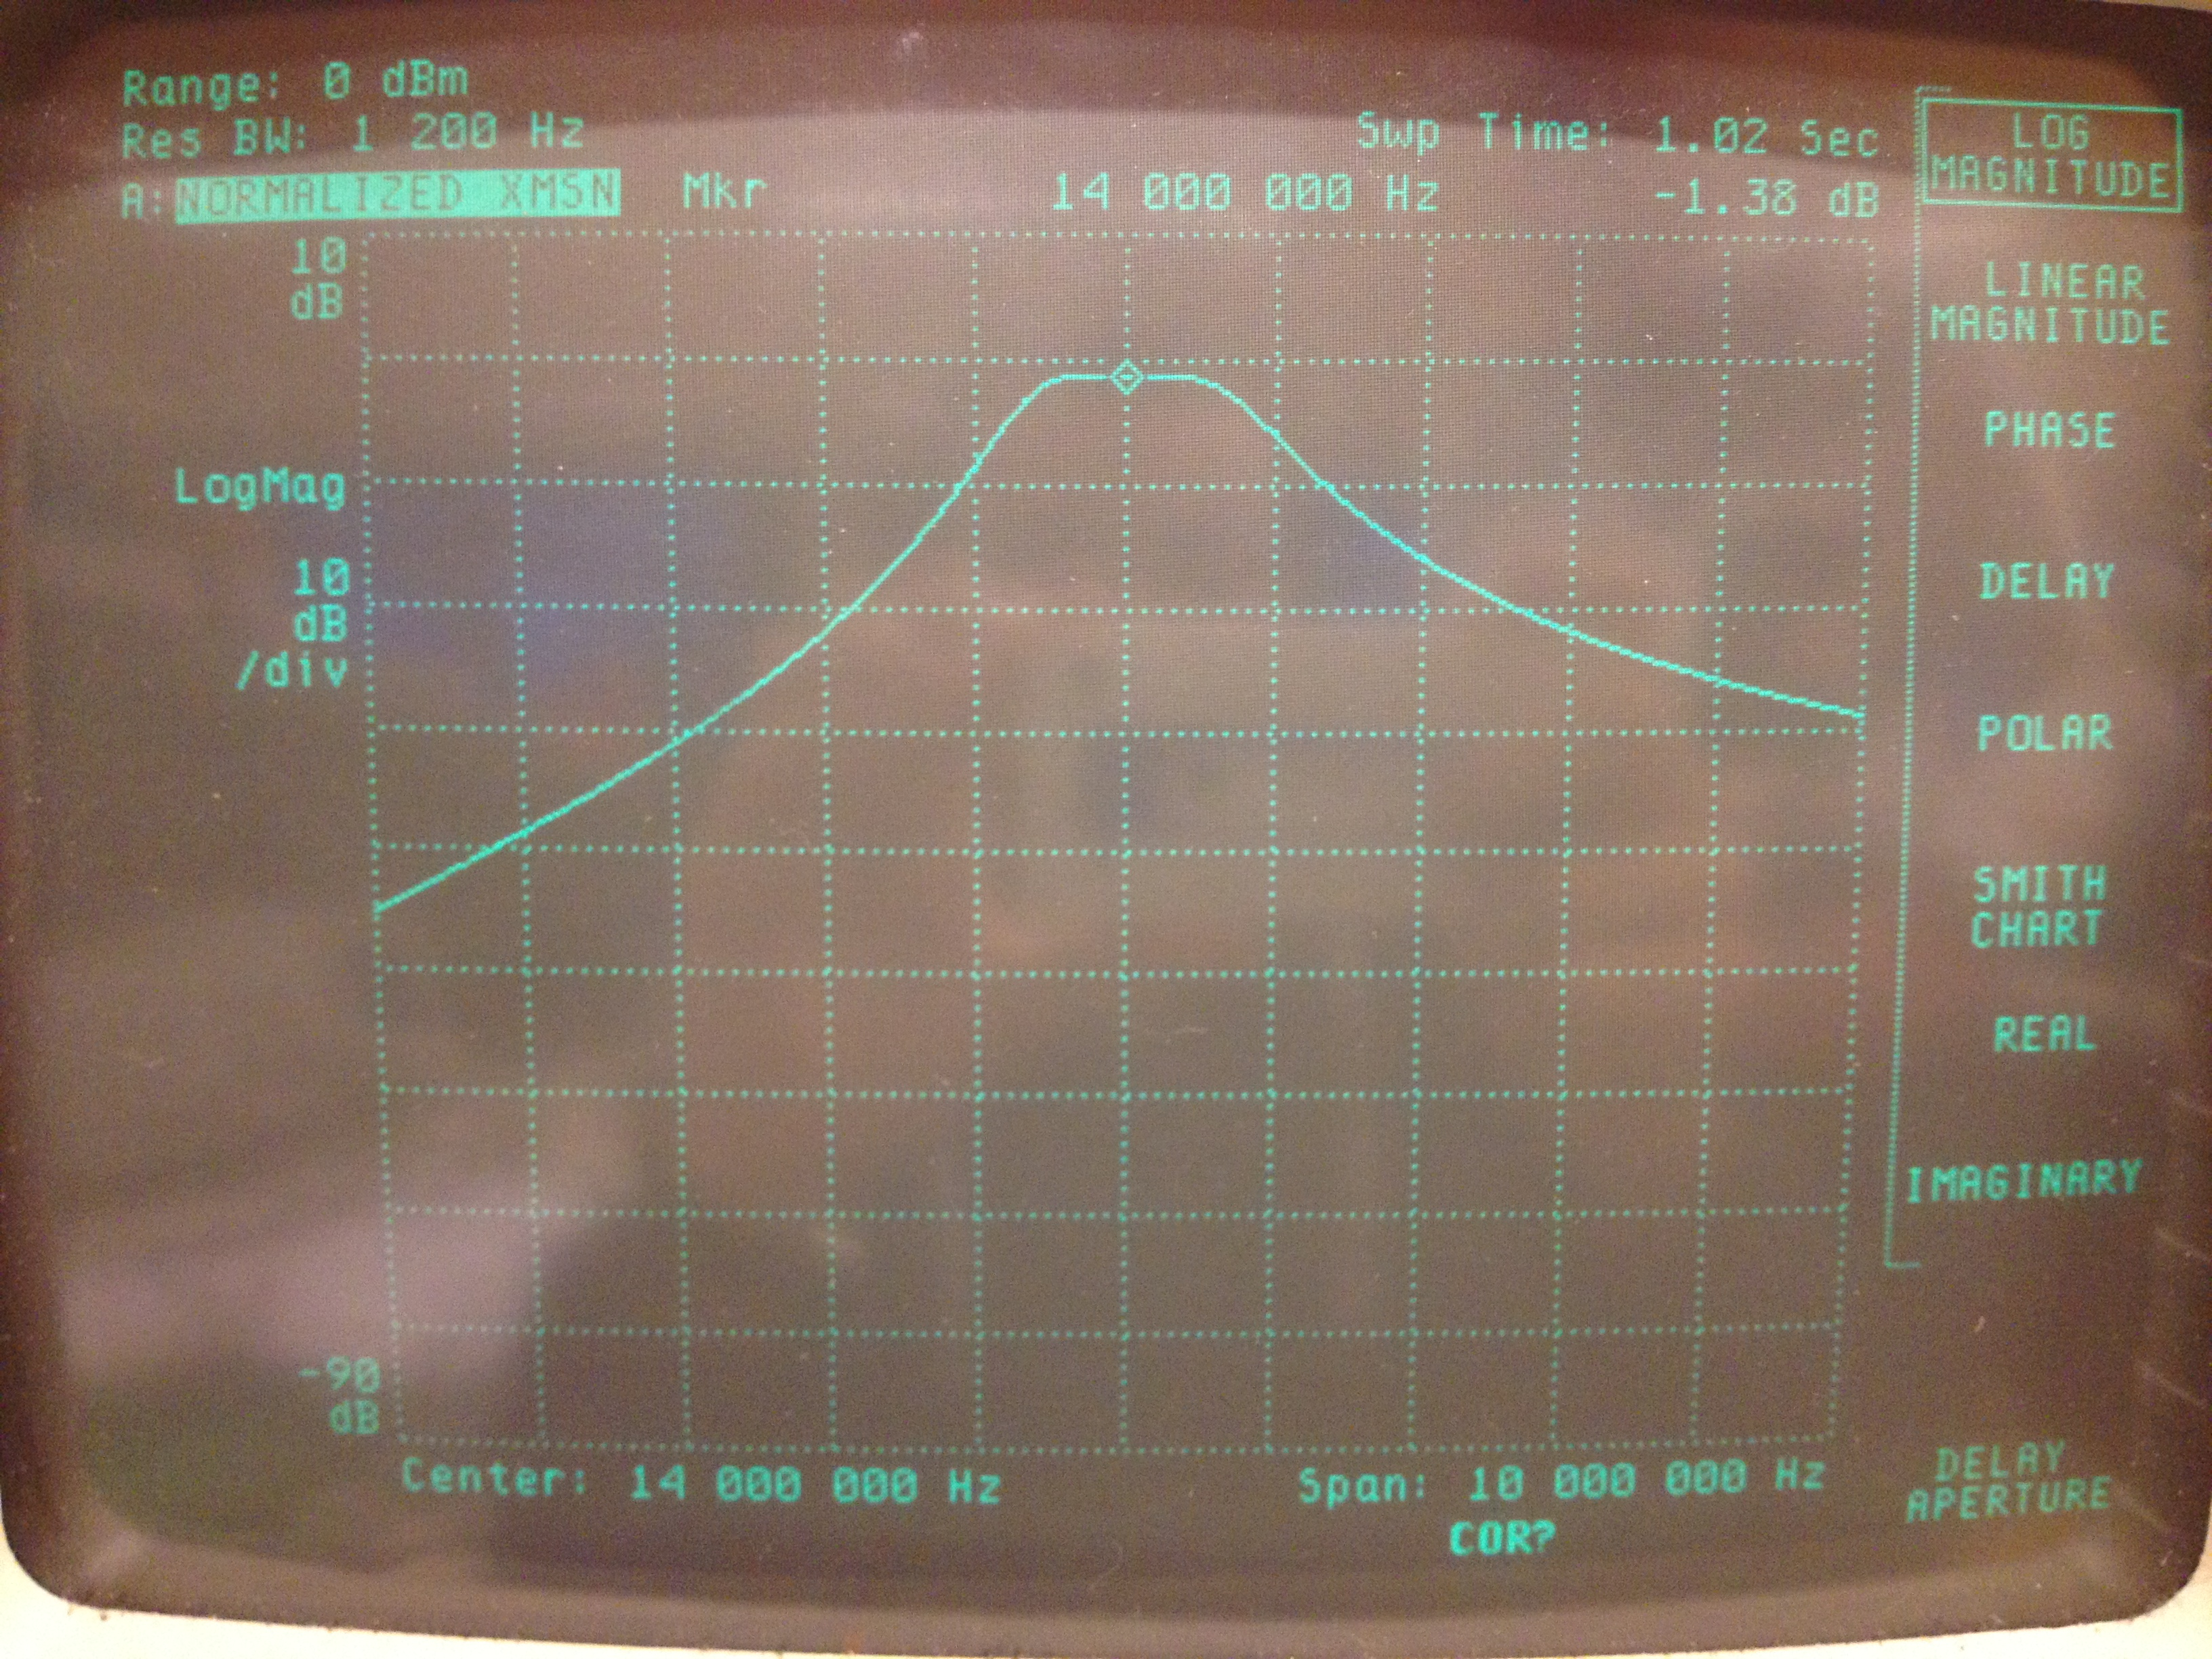
\includegraphics[width=\textwidth]{bande_2MHz_bienregle}
		\caption{Module}
	\end{subfigure}
	\hfill
	\begin{subfigure}[b]{0.43\textwidth}
		\centering
		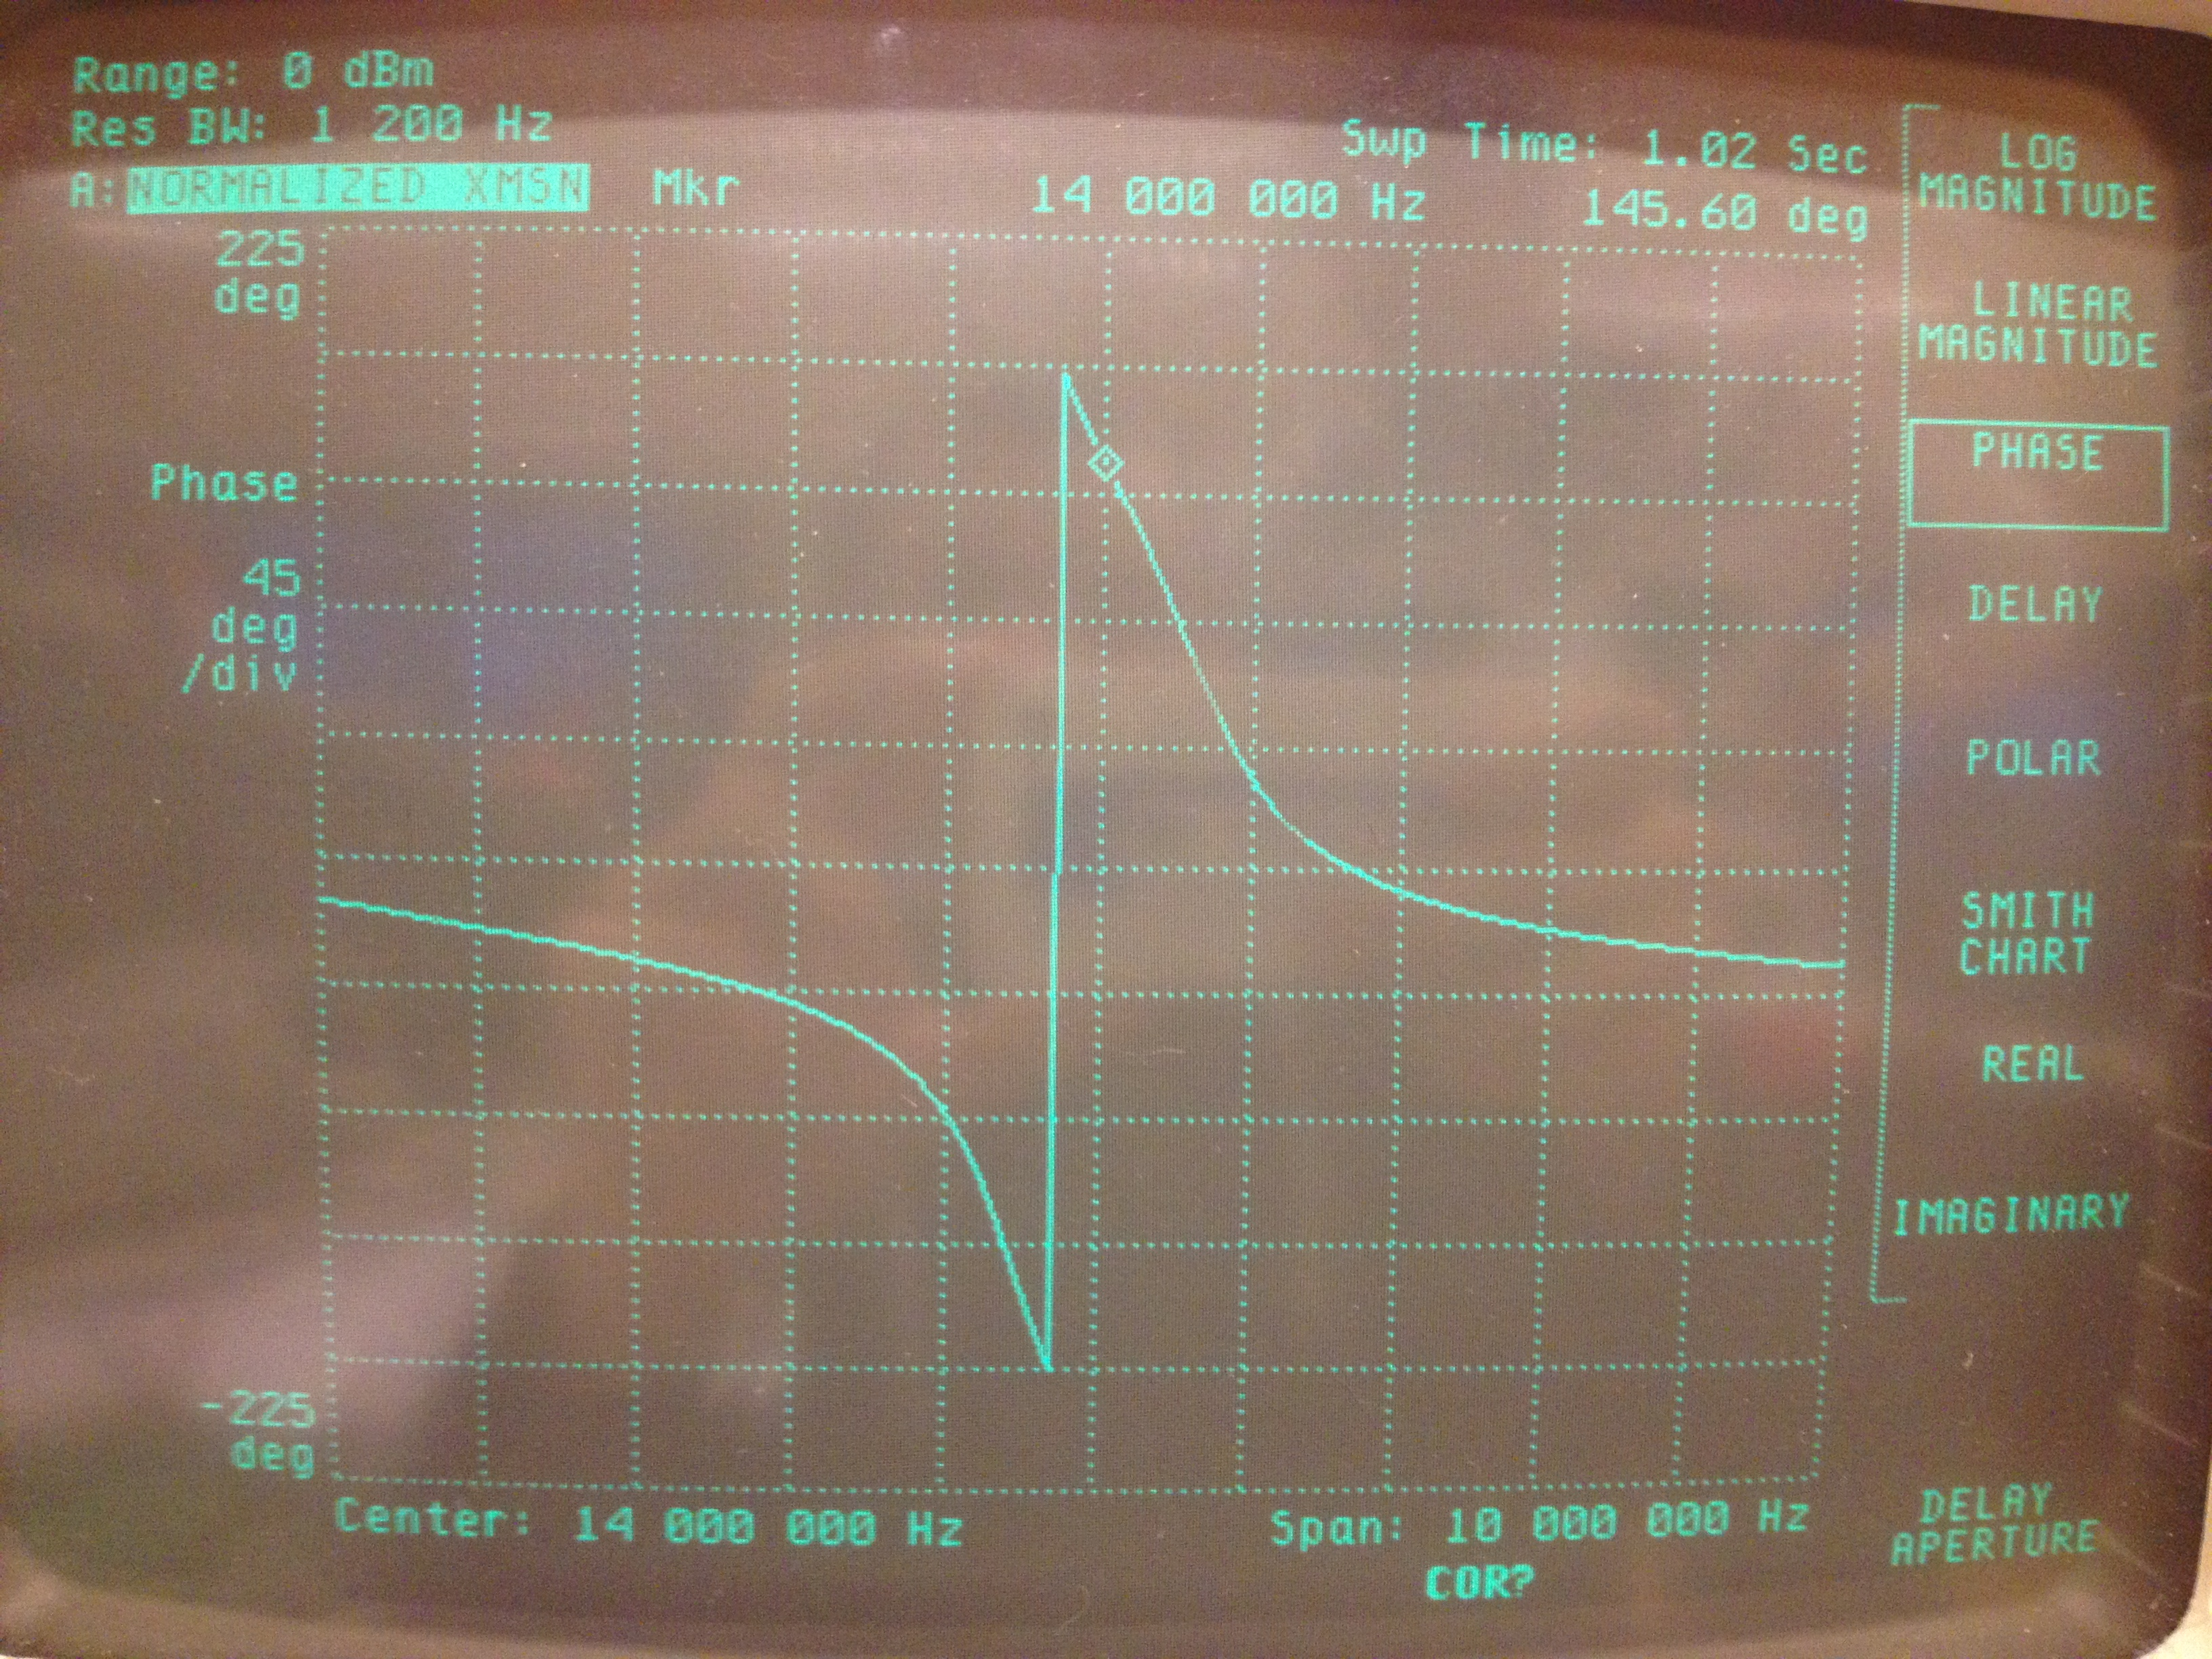
\includegraphics[width=\textwidth]{phase_bienregle}
		\caption{Phase}
	\end{subfigure}
	\caption{Diagramme de Bode du filtre LC à deux circuits accordés couplés réglé}
	\label{fig:LCregle}
\end{figure}



\exsubpart{4}

Les pertes d'insertion de ce filtre se lisent sur le tracé Fig.~\ref{fig:LCregle}. En effet, puisque l'on peut, à 14MHz, négliger les pertes liées aux diviseurs capacitifs, ces pertes d'insertion correspondent aux pertes observer au plus fort de la résonance~: -1,38 dB.








\section{L'amplificateur accordé}

\subsection{Description}

On considère l'amplificateur accordé décrit Fig.~\ref{schem6}.

\begin{figure}[h!]
	\centering
	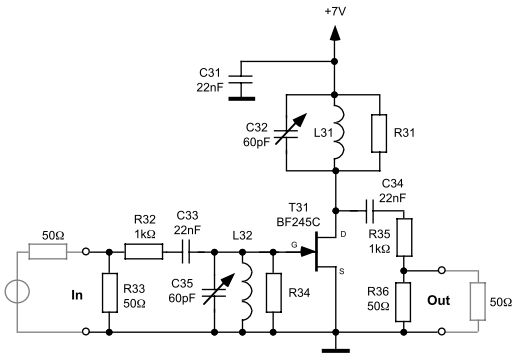
\includegraphics[width=.7\textwidth]{schem6}
	\caption{L'amplificateur accordé}
	\label{schem6}
\end{figure}


\subsection{Questions et calculs}

\exsubpart{1}

Les deux circuits résonnants sont couplés via un couplage actif.

\exsubpart{2}

On couple deux filtres d'ordre 2, formant ainsi un filtre d'ordre 4.

Si le facteur de qualité de chacun des circuits résonants est le même, on obtient donc un facteur de qualité global de~:
\begin{equation*}
Q_{tot} = \frac{1}{\sqrt{2^{1/2}-1}}Q = 1,554 Q
\end{equation*}


\exsubpart{3}

Les condensateurs C33 et C34, compte tenu de leur taille, permettent uniquement de couper de très basses fréquences, hors de notre domaine d'intérêt. On peut donc les ignorer.

Les filtres restants en amont et en aval du JFET sont tous deux constitués d'une inductance et d'une capacité en parallèle, liées à une tension de référence. Ce sont deux passe-bande d'ordre 2~: l'ordre est de 1 de chaque côté de la fréquence de résonance, donnant donc lieu à des pentes de $\pm$20 dB/décade de part et d'autre de cette fréquence.

En couplant ces deux filtres, on obtient donc un filtre passe-bande d'ordre total 4. On trouve de part et d'autre de la fréquence de résonance $f_0$ un ordre 2, soit des pentes de +40 dB/ec et -40 dB/dec respectivement en-dessous et au-dessus de $f_0$.


\exsubpart{4}

Afin d'obtenir une bande passante à -3dB s'étendant de $f_1 = $13 MHz à $f_2 = $15 MHz, le facteur de qualité total doit être de~:
\begin{equation*}
Q_{tot} = \frac{f_0}{f_2-f_1}
\end{equation*}
avec $f_0 = $14 MHz, soit~:
\begin{equation*}
Q_{tot} = 7
\end{equation*}

Cela correspond pour chaque circuit résonant à un facteur de qualité de~:
\begin{equation*}
Q = \sqrt{2^{1/2}-1}~Q_{tot} = 4,505
\end{equation*}



\exsubpart{5}

Pour les petits signaux, à la fréquence de résonance --- où C32||L31 et C35||L32 sont assimilés à des circuits ouverts --- le montage est équivalent au circuit donné Fig.~\ref{fig:eqFET}.

\begin{figure}[h]
	\centering
	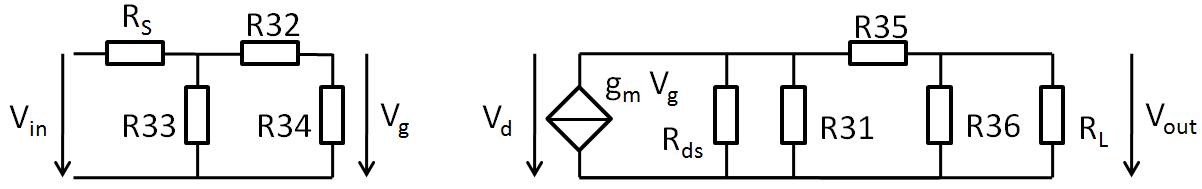
\includegraphics[width=.8\textwidth]{eqFet}
	\caption{Équivalence pour les petits signaux à la fréquence de résonance}
	\label{fig:eqFET}
\end{figure}

Le gain en tension théorique $A_v=\frac{V_d}{V_g}$ est alors donné par~:
\begin{equation*}
A_v = \frac{g_m}{\frac{1}{R_{ds}}+\frac{1}{R_{31}}+\frac{1}{R_{35}+\frac{1}{R_{36}^{-1}+R_{L}^{-1}}}}
\end{equation*}


\subsection{Mesures et réglages}

\exsubpart{1}

Un fois réglé, l'amplificateur accordé donne les résultats présentés Fig.~\ref{fig:6loglog}.

\begin{figure}[h]
	\centering
	\includegraphics[width=.5\textwidth]{6_3_3_reponse_ampli_loglog_}
	\caption{Réponse de l'amplificateur accordé de 1MHz à 100MHz}
	\label{fig:6loglog}
\end{figure}

On observe bien en basses et hautes fréquences les pentes $\pm$40 dB/dec prédites, relativement noyées dans du bruit et éloignées de la fréquence de résonance --- la résonance étant ici relativement large.


%TODO: partie 2) : image manquante !

\exsubpart{3}

On mesure à la fréquence de résonance un gain total $A_{tot}$ de -23,3 dB.

Or le pont diviseur R35-R36-RL engendre un gain~: $A_R = \frac{(R_{36}||R_L)}{R_{35}+(R_{36}||R_L)} = $ -32,3 dB

Le gain $A_v$ est donc de~: $A_v = \frac{A_{tot}}{A_R} = 9~\mathrm{dB} = 2,8$

\exsubpart{4}

On applique en entrée de l'amplificateur accordé un signal sinusoïdal de fréquence 14MHz et puissance 0 dBm. On obtient le spectre donné Fig.~\ref{fig:6_0dbm}. La composante à 14MHz est bien réduite d'approximativement 23,3 dB. En revanche, à cette composante s'ajoute une harmonique à 28MHz, plus faible de 47 dB.

En augmentant à 10 dBm la puissance en entrée, on obtient le spectre donné Fig.~\ref{fig:6_10dbm}. L'harmonique à 28MHz est renforcée, et d'autres harmoniques apparaissent.


\begin{figure}[h]
	\centering
	\begin{subfigure}[b]{0.43\textwidth}
		\centering
		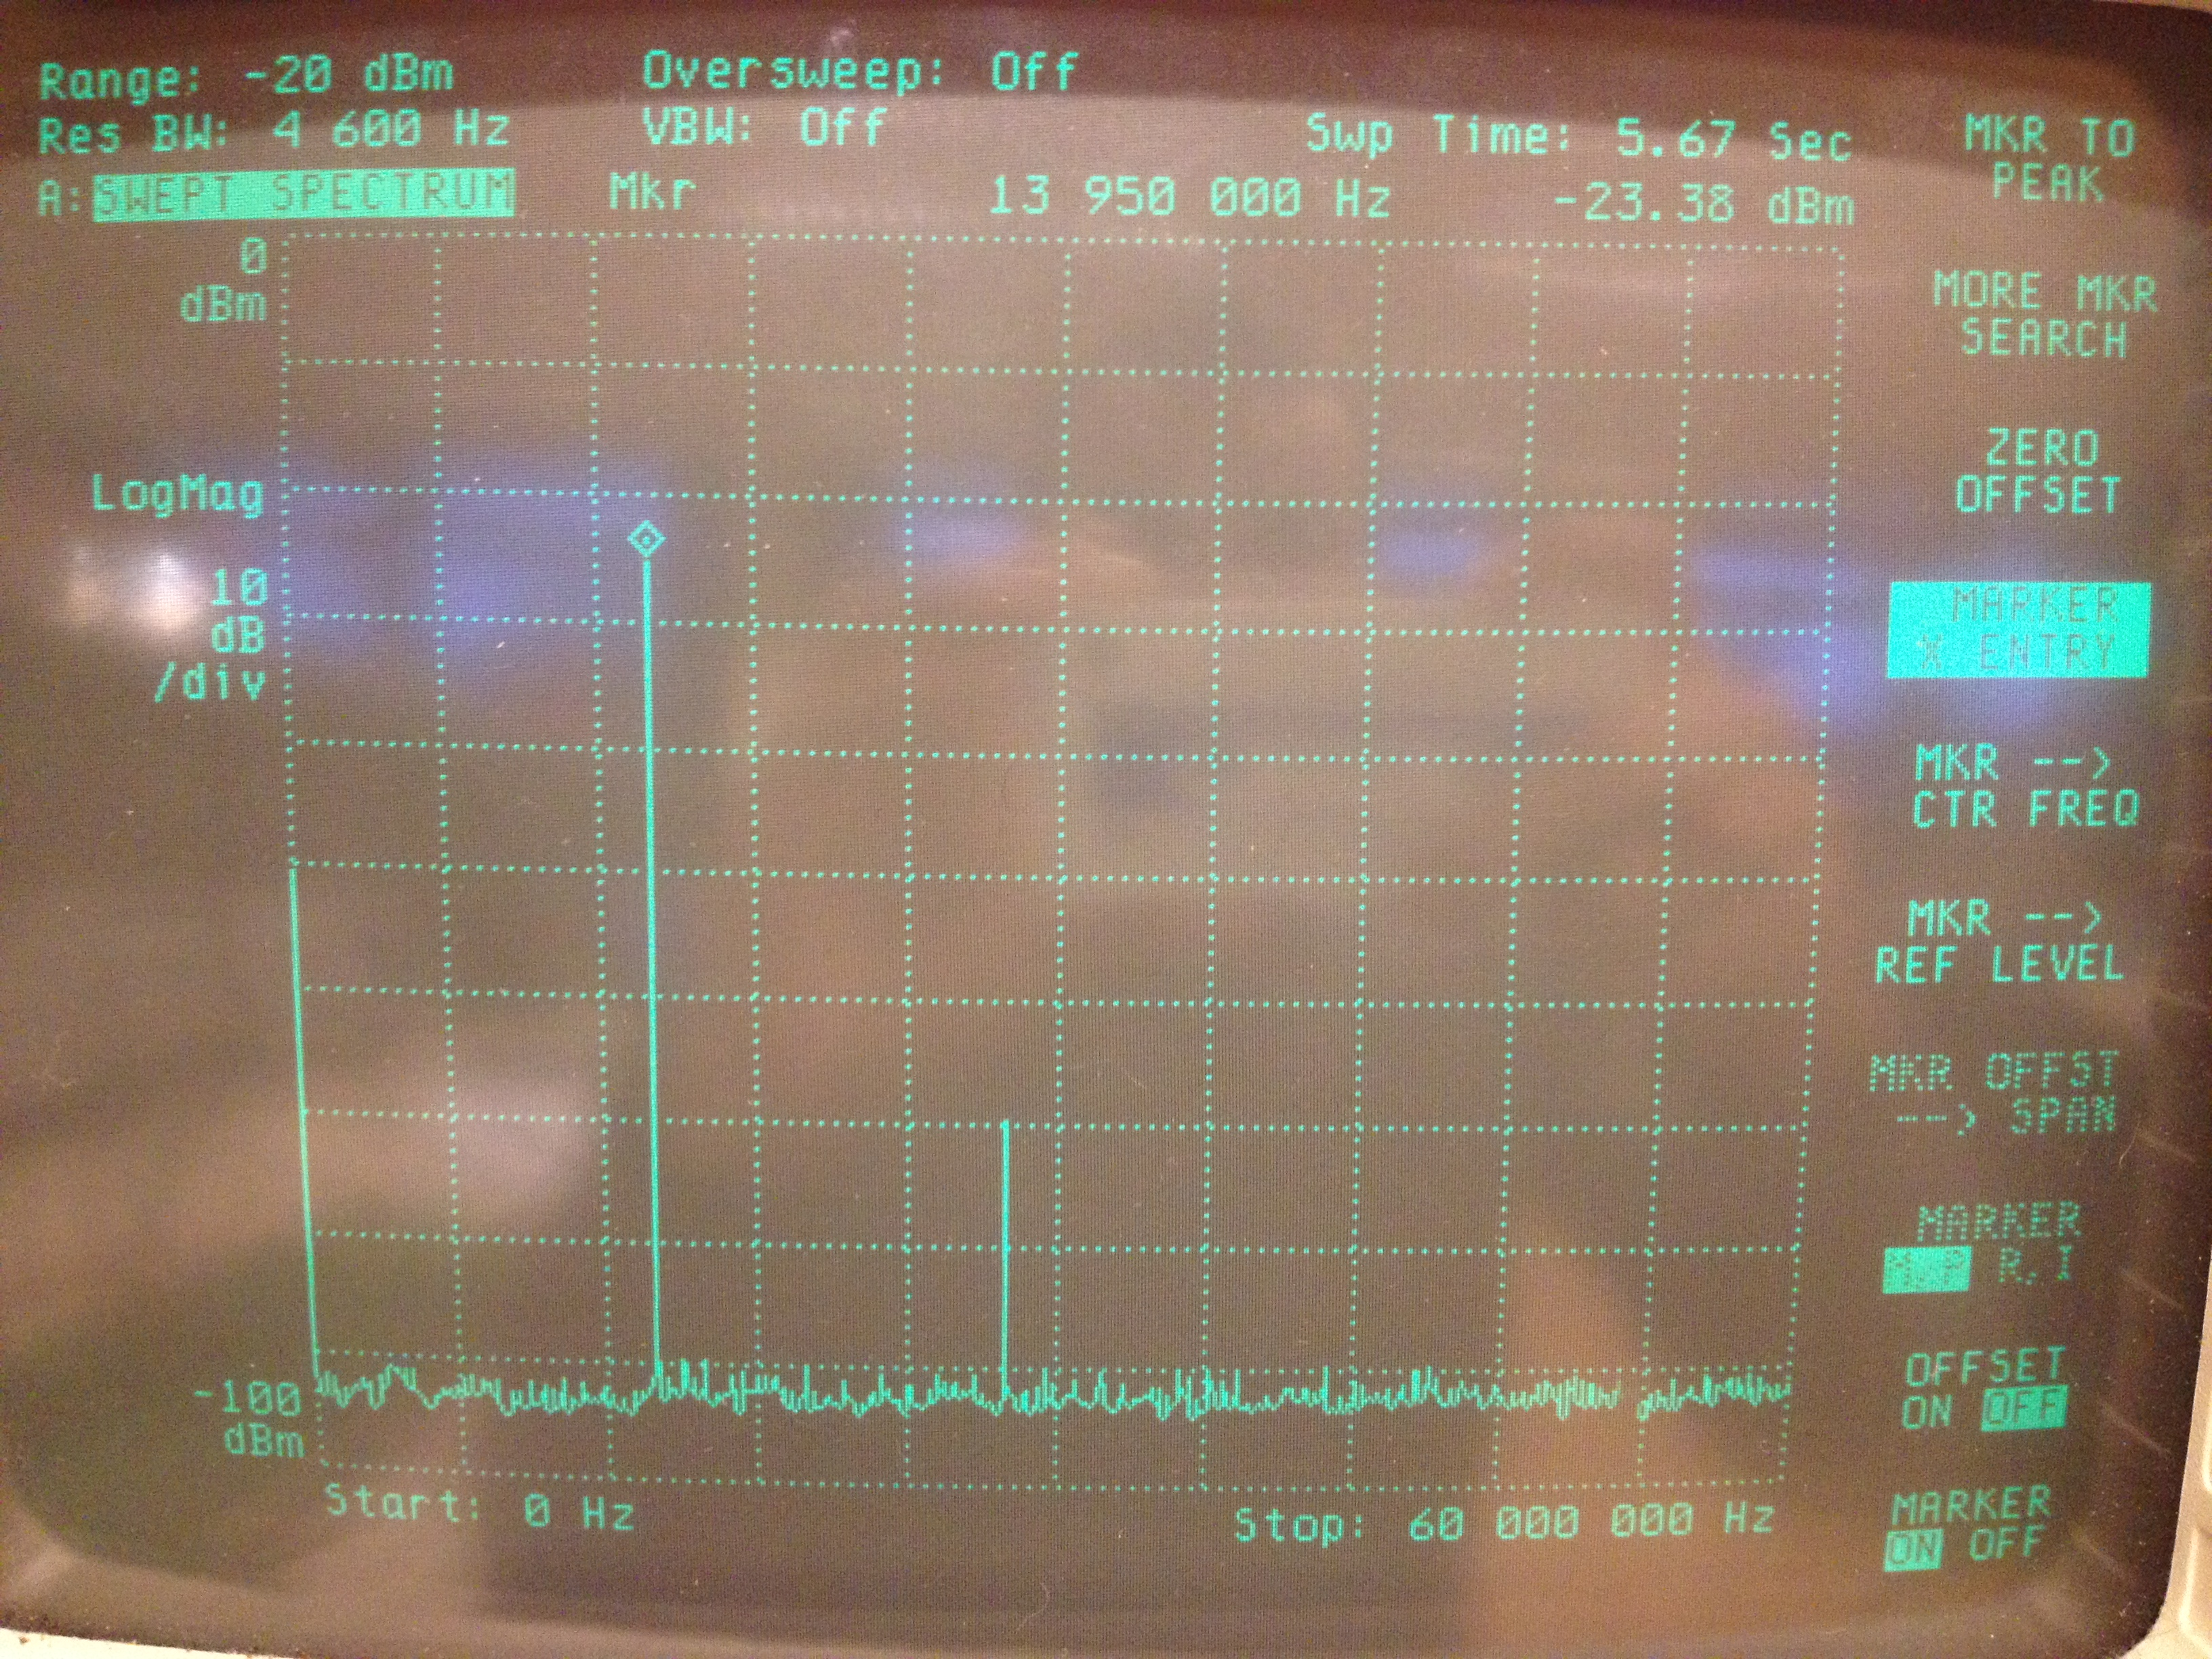
\includegraphics[width=\textwidth]{6_3_2_2MHz_0dbm}
		\caption{Pour une entrée à 0 dBm}
		\label{fig:6_0dbm}
	\end{subfigure}
	\hfill
	\begin{subfigure}[b]{0.43\textwidth}
		\centering
		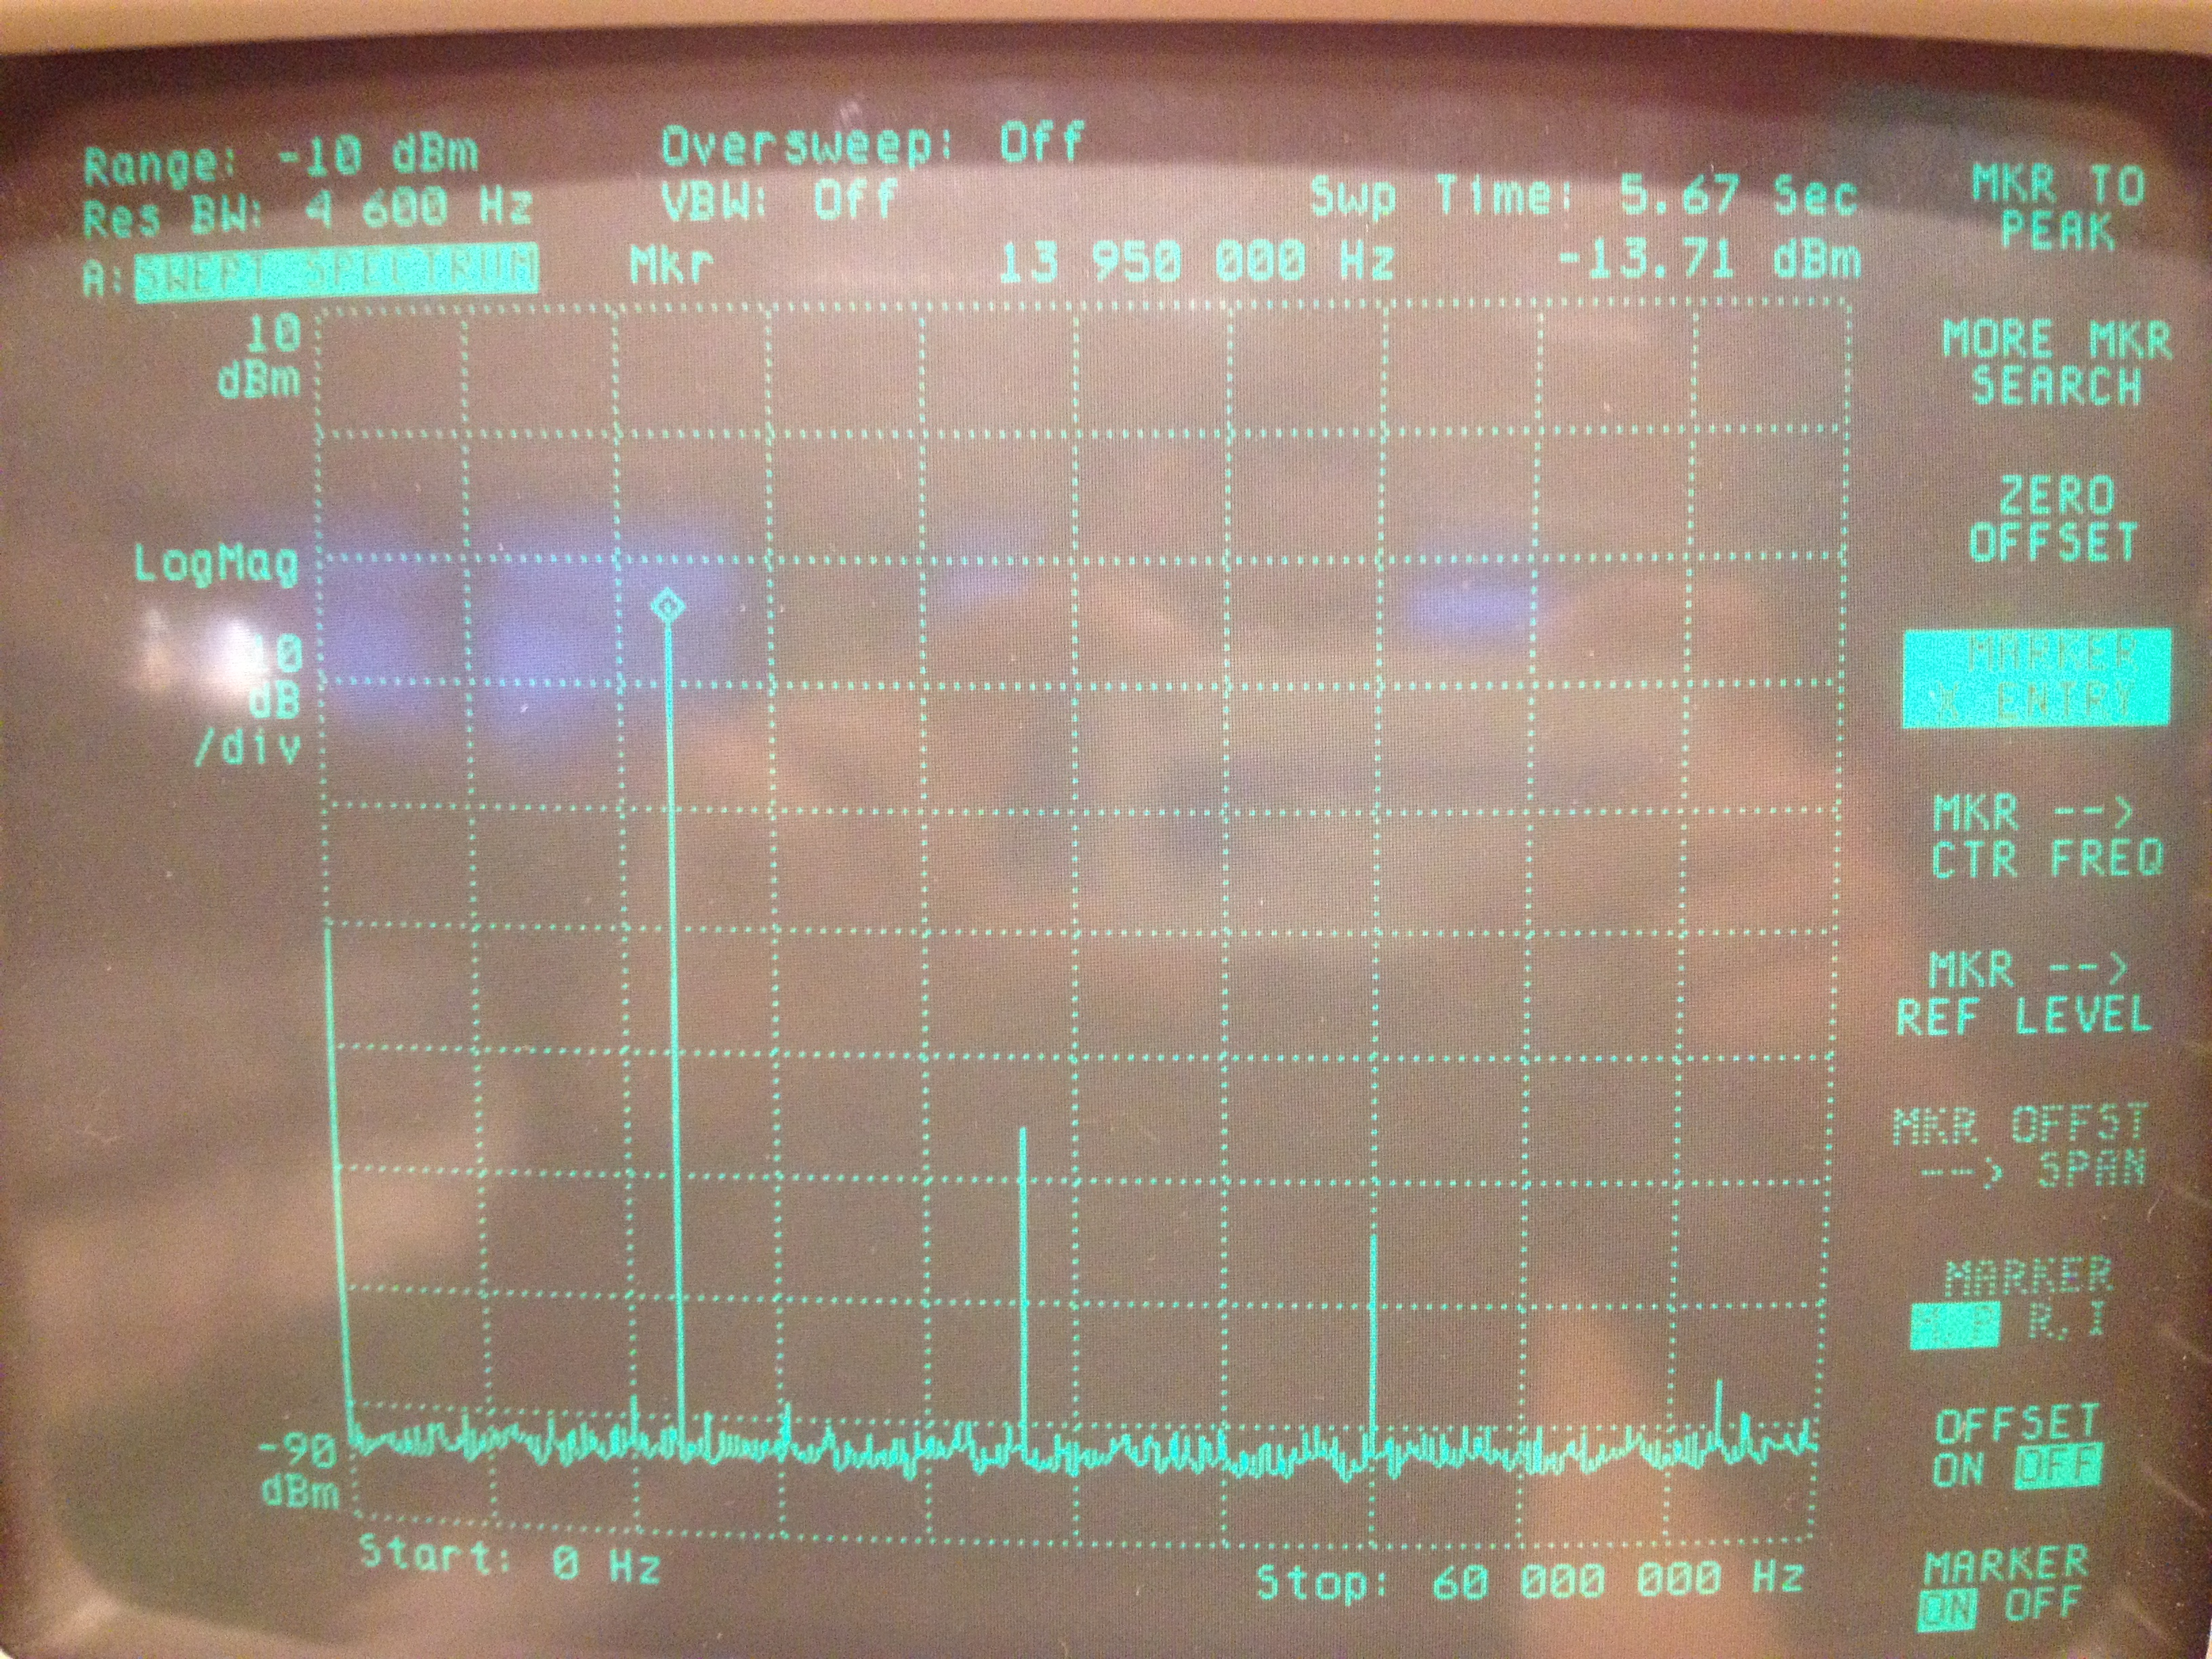
\includegraphics[width=\textwidth]{6_3_2_2MHz_10dbm}
		\caption{Pour une entrée à 10 dBm}
		\label{fig:6_10dbm}
	\end{subfigure}
	\caption{Spectre de la réponse à un signal sinusoïdal à 14MHz}
\end{figure}



\exsubpart{5}

On atteint le compression à 1dB pour une entrée à 11,5 dBm, soit une tension de 2,38V crête à crête.


\exsubpart{6}

On injecte désormais en entrée un signal double-ton à 13,9MHz et 14,1MHz. On observe en sortie les spectres présentés Fig.~\ref{fig:6_double}.

\begin{figure}[h]
	\centering
	\begin{subfigure}[b]{0.43\textwidth}
		\centering
		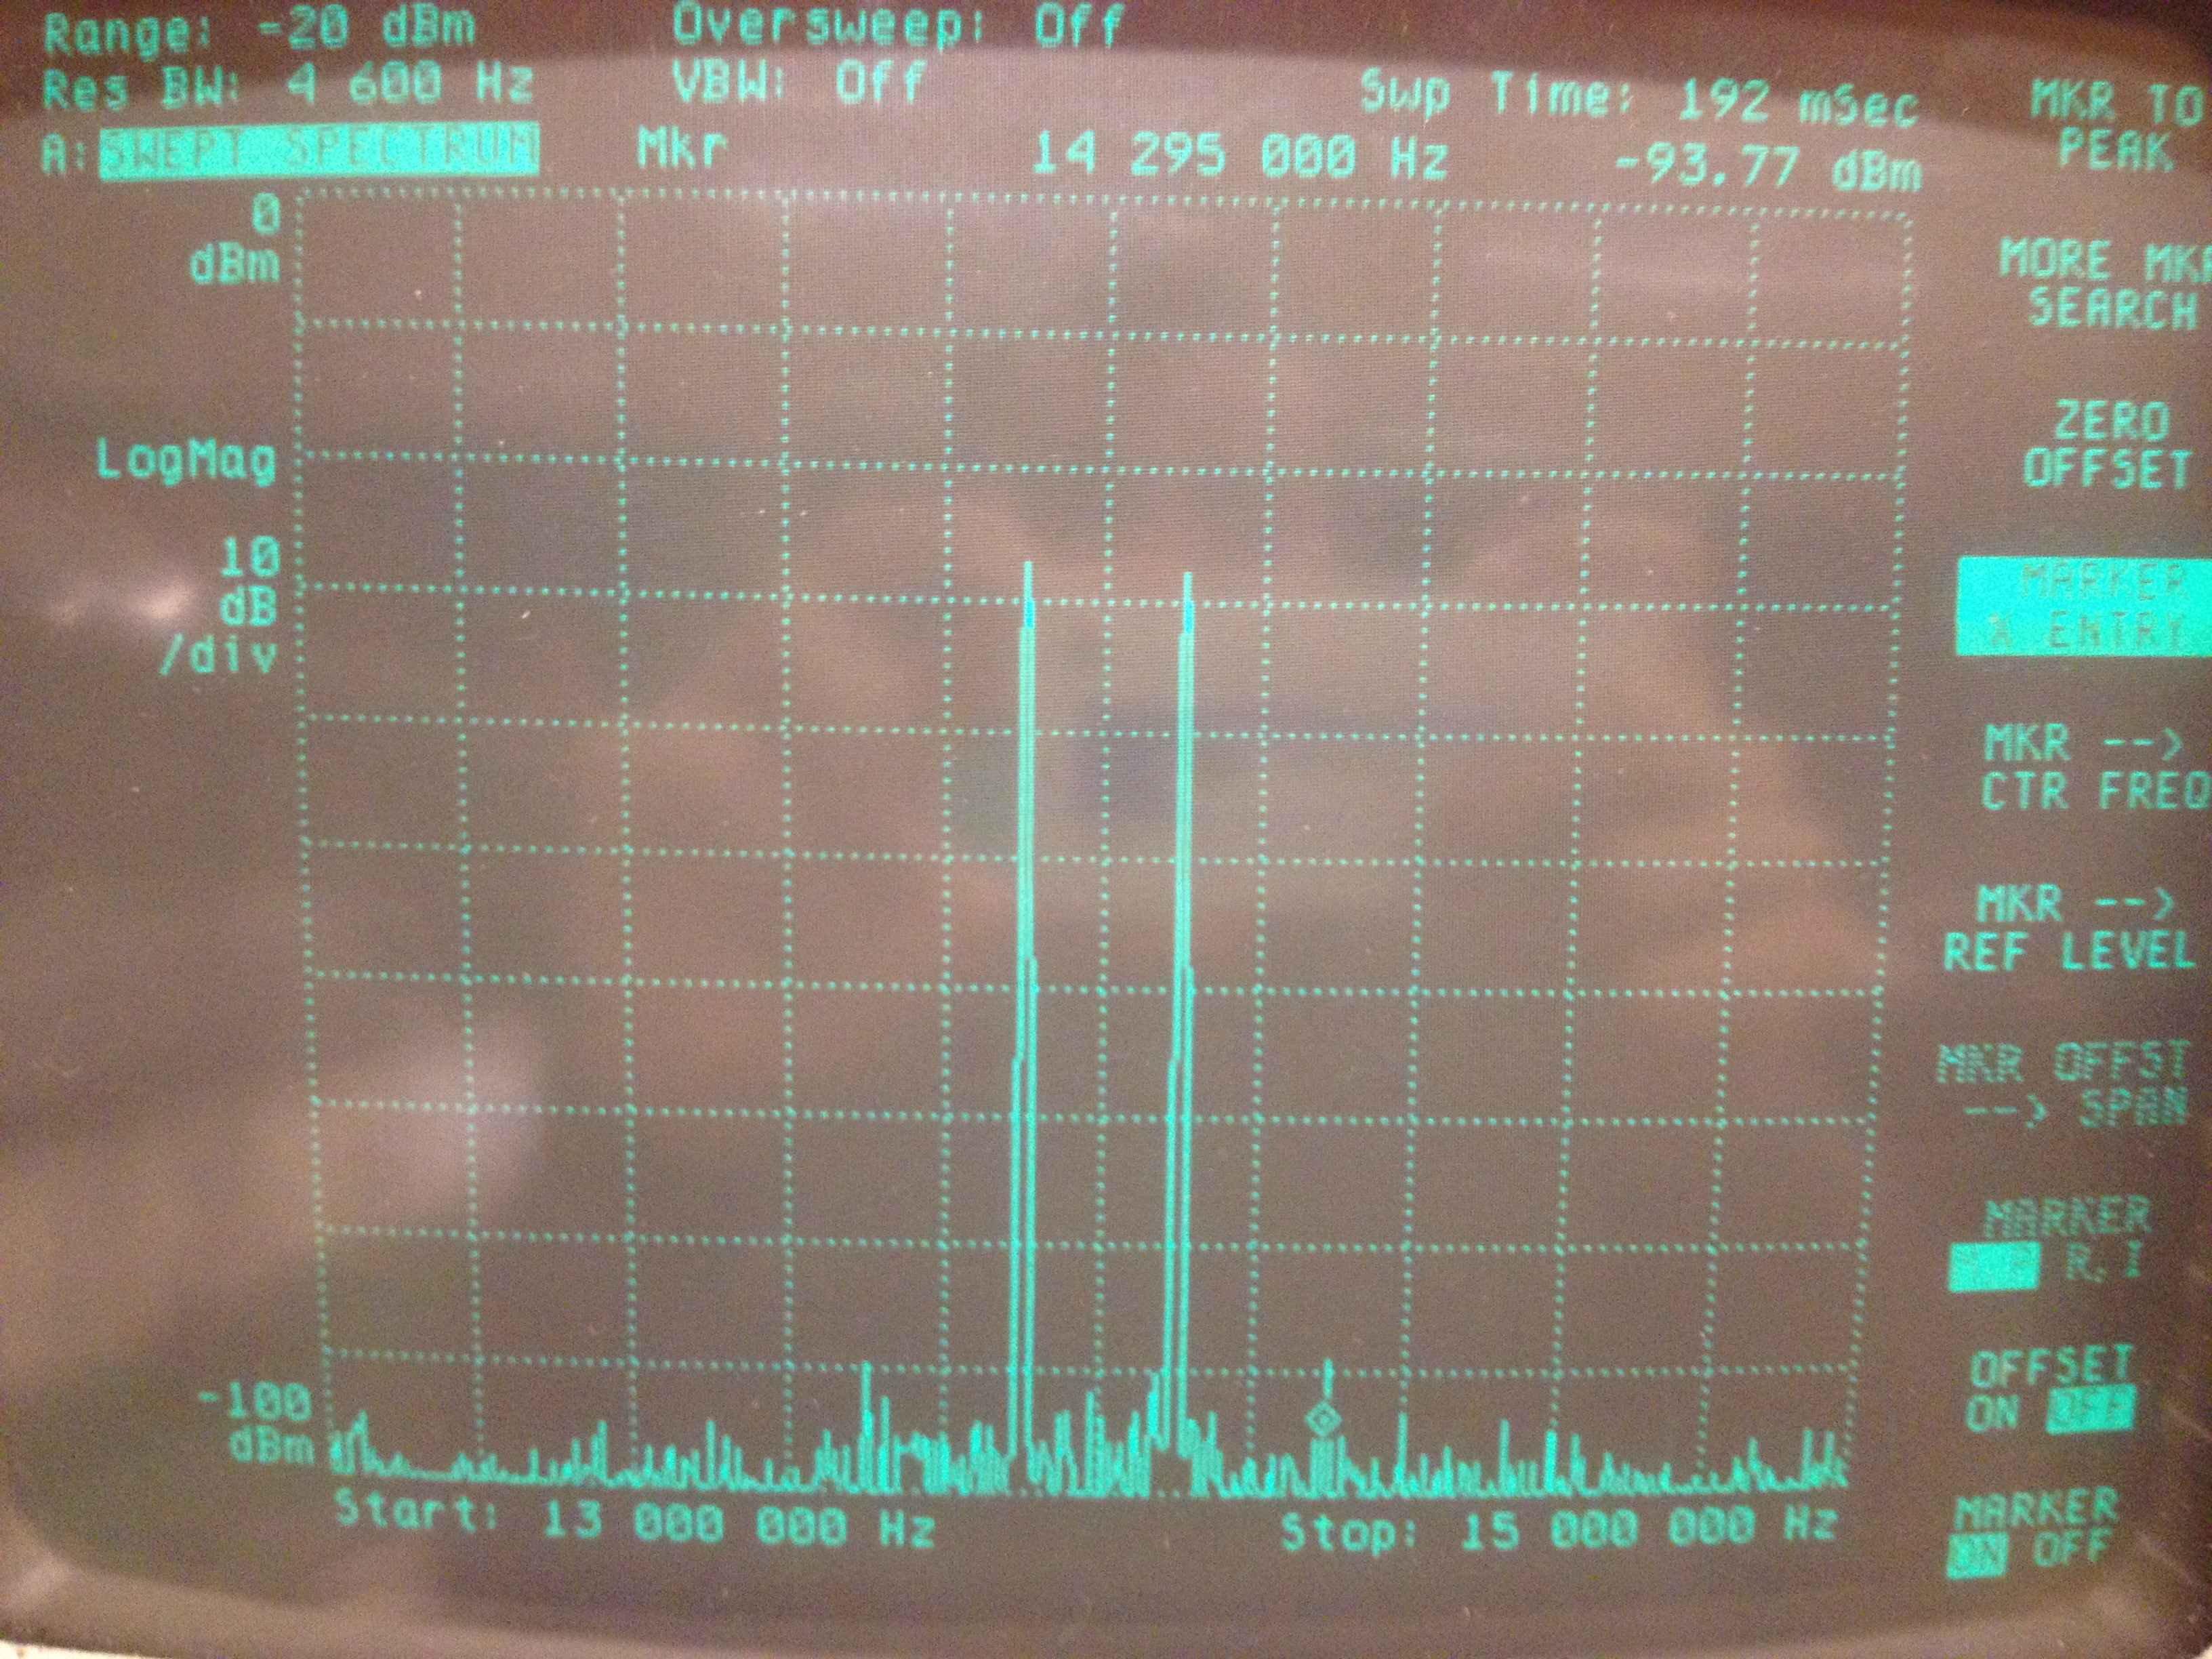
\includegraphics[width=\textwidth]{6_3_6_0dbm}
		\caption{Pour une entrée à 0 dBm}
	\end{subfigure}
	\hfill
	\begin{subfigure}[b]{0.43\textwidth}
		\centering
		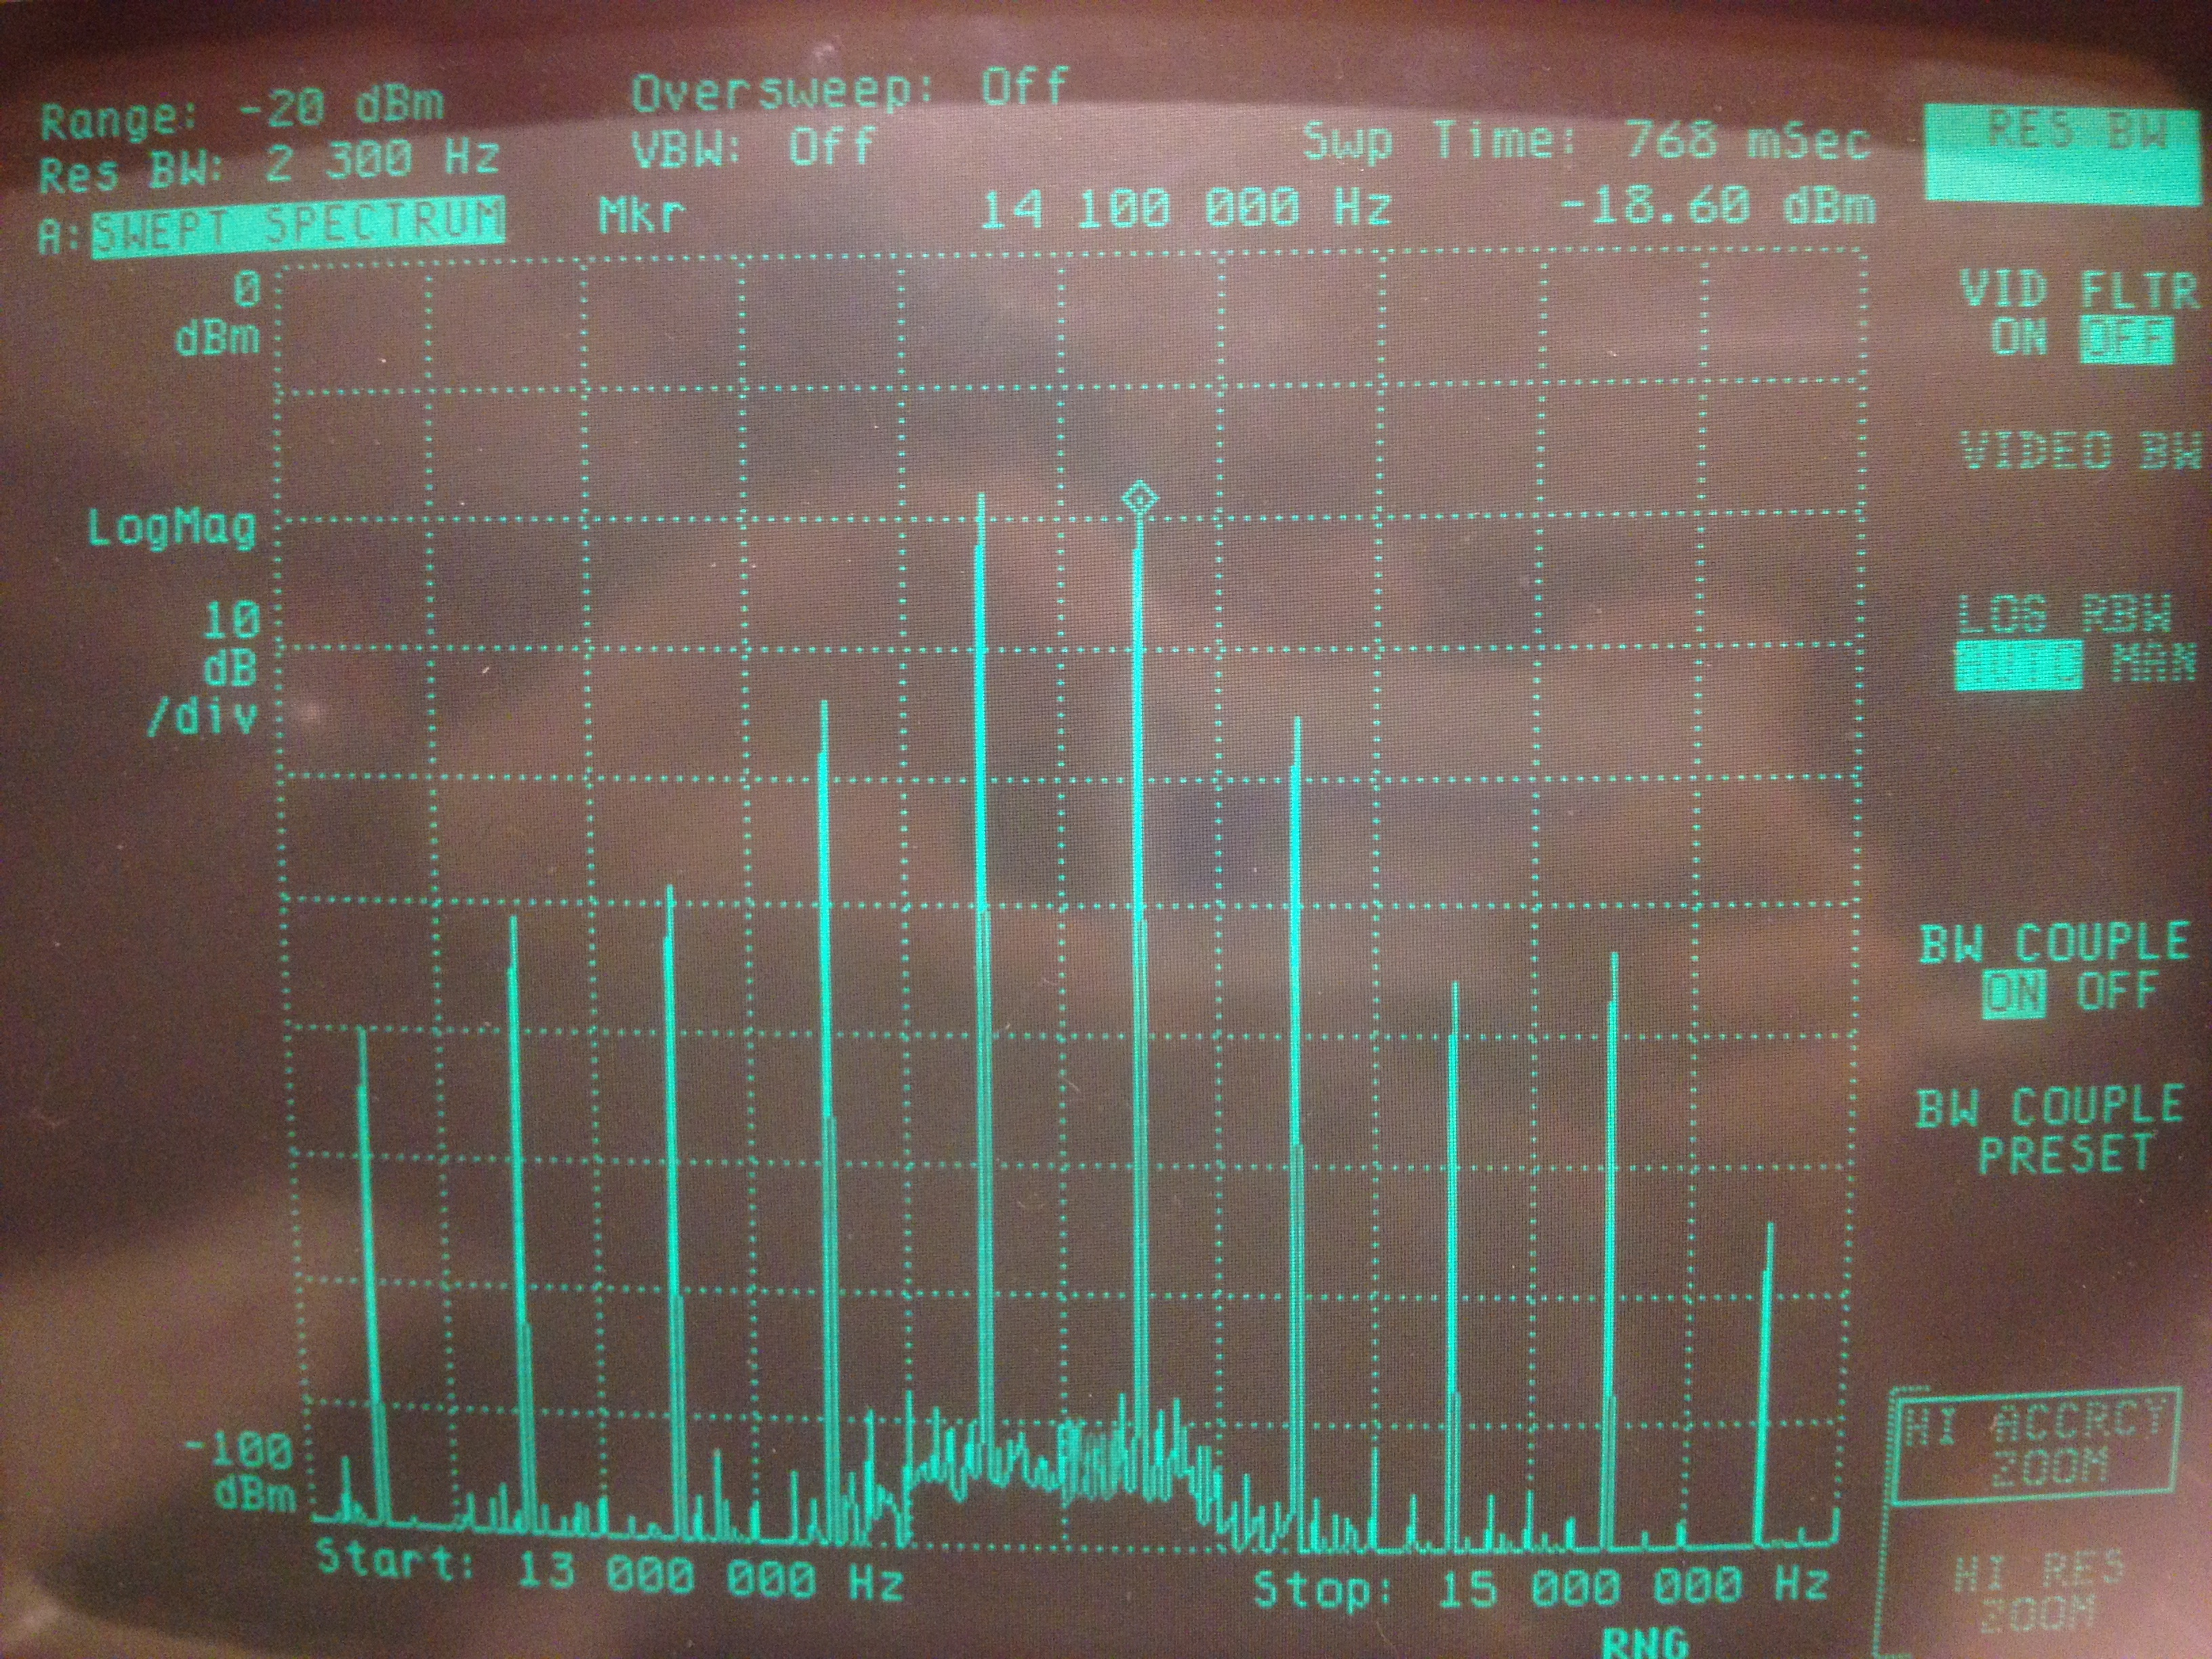
\includegraphics[width=\textwidth]{6_3_6_11x5dbm}
		\caption{Pour une entrée à 11,5 dBm}
	\end{subfigure}
	\caption{Spectre de la réponse à un signal double-ton à 13,9MHz et 14,1MHz}
	\label{fig:6_double}
\end{figure}

Pour une entrée simple-ton à 14MHz et de 0 dBm, on a vu mesuré en sortie à 14MHz une fondamentale de -23,3 dBm. Pour une entrée double-ton à 13,9MHz et 14,1MHz et de 0 dBm, on obtient en sortie un produit d'intermodulation d'ordre 3 de -89,9 dBm.

On déduit que le point du troisième ordre se situe à $\frac{89,9-23,3}{2}~=~33,3~\mathrm{dBm}$, soit 29,9V crête à crête.








\section{L'oscillateur à quartz}

\subsection{Description}
To do

\subsection{Questions et calculs}

\exsubpart{1}

La réaction positive s'effectue par le condensateur parasite $C_{bc}$ qui se trouve entre le collecteur et la base du transistor.
\begin{center}
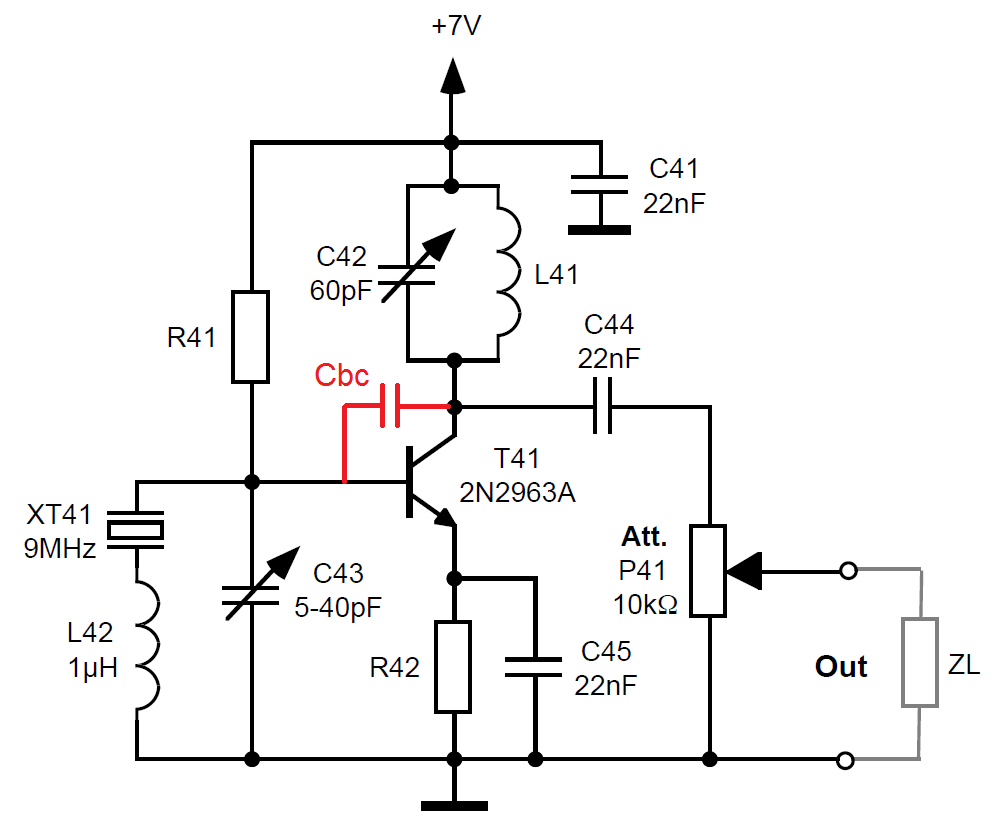
\includegraphics[width = 0.7\linewidth]{shema_oscillateur.png}
\end{center}
L'oscillateur est de type Colpitts, c'est à dire que la réaction positive est réalisée par un diviseur capacitif.\\
Si on considère le schéma petits signaux (suppression des composantes continues servant à polariser le transistor), on obtient le schéma suivant :
\begin{center}
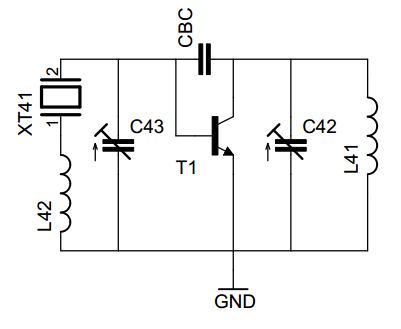
\includegraphics[width=0.4\linewidth]{shema_petit_signaux_oscillateur.png}
\end{center}
On voit alors que le circuit de charge est un filtre passe-bande formé par $L_{41}$ et $C_{42}$. Les fréquences seront toutes atténuées, sauf celles proches de la fréquence de résonance $f_0$, où $f_0 = \frac{1}{2 \pi \cdot \sqrt{L_{41} \cdot C_{42}}}$.
En admettant qu'à l'enclenchement du circuit, il y a du bruit blanc sur la base du transistor, ce bruit blanc inclut toutes les fréquences y compris $f_0$. Il ne restera plus que $f_0$ à la sortie, qui sera alors ré-injectée dans la base par le diviseur formé par $C_{BC}$ et $C_{43}$.\\
La condition pour que l'oscillation démarre est que le gain du transistor doit être plus grand que l'atténuation du diviseur captatif. La branche avec le quartz n'est pas nécessaire pour l'apparition d'une oscillation. Cependant elle sert a sélectionner une fréquence particulière de façons plus précise.

En effet, le quartz agit comme un filtre supplémentaire, et son facteur de qualité Q est très largement plus élevé que celui d'un filtre à composant LC (qui présentent des imperfections électromécaniques).\\

Le quartz peut être modélisé de la façon suivante :\footnote{Source : $www.acedim.com/Formatronic/Electro_2/oscillateur/lequartz.html$}
\begin{center}
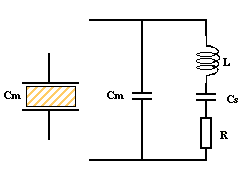
\includegraphics[width=0.4\linewidth]{modele_quartz.png}
\end{center}
Il a alors deux fréquences de résonances : fp$=\frac{1}{2\pi \cdot L_s \cdot C_s}$ et fs$=\frac{1}{2\pi \cdot L_s \cdot C_{eq}}$, où $C_{eq} = \frac{1}{\frac{1}{C_s} + \frac{1}{C_m}}$. Ces deux fréquences sont en général très proches l'une de l'autre.\\
Le quartz est capacitif sur toutes les plages de fréquences sauf dans la bande très étroite qui se trouve entre fp et fs \footnote{Source : $http://www.acedim.com/Formatronic/Electro_2/oscillateur/oscilaquartz.html$}:
\begin{center}
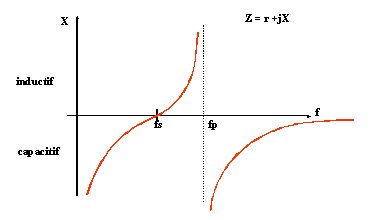
\includegraphics[width=0.4\linewidth]{impedence_quartz.png}
\end{center}

Le quartz a un comportement inductif à la fréquence d'oscillation, qui est donc toujours comprise entre fp et fs.\\

Il est nécessaire que le résonateur $L_{41}$ et $C_{42}$ soit accordé à une fréquence très proche de celle du quartz, sinon les deux filtres vont s'annuler réciproquement et il n'y aura pas d'oscillations.

\exsubpart{2}

Le condensateur $C_{42}$ a peu d'influence sur la fréquence de sortie. En effet, changer son réglage changera $f_0$, mais le filtre réalisé par le Quartz ayant un facteur de qualité beaucoup plus grand, c'est lui qui sera déterminant pour la fréquence des oscillations. Si $C_{42}$ est mal réglé, nous aurons simplement une atténuation de l'amplitude des oscillations, ou carrément un arrêt de l'oscillateur.\\
En revanche, le réglage de $C_{43}$ vient affecter directement le quartz et va donc avoir un effet direct sur la fréquence d'oscillation.

\exsubpart{3}

Le fait de brancher une charge à la sortie va diminuer le facteur de qualité du résonateur $L_{41}$ et $C_{42}$ et donc affecter le rapport de force entre ce filtre et le quartz.Plus la résistance de charge est faible, plus le facteur de qualité baisse donc plus la fréquence sera proche de celle du Quartz, ce qui est l'idéal.

\exsubpart{4}

%\subsection{Dimensionnement de la polarisation}
On fait une analyse en grand signaux, c'est à dire que toutes les inductances sont des court-circuits, et les capacités ainsi que le quartz sont circuits ouverts.\\
Le courant de repos Ic de $1mA$ doit circuler dans le collecteur et l'émetteur du transistor. On désire avoir 1V sur l'émetteur, d'où la valeur de $R_{42}$ :
\begin{center}
$R_{42} = \frac{U_e}{Ic} = \frac{1V}{1mA} = 1k\Omega$
\end{center}
Puis, le courant circulant dans la base du transistor, et donc dans $R_{41}$ est $\beta$ fois plus petit que Ic.\\
Le facteur $\beta$ varie fortement avec la température et d'un transistor à l'autre, cependant on peut pour ce transistor estimer que $\beta \simeq 100$ d'où :
\begin{center}
$Ib = \frac{Ic}{\beta} = \frac{1mA}{100} = 10\mu A$
\end{center}
La tension entre la base et l'émetteur est identique à celle d'une diode en conduction $Uj \simeq 0.7V$, d'où :
\begin{center}
$R_{41} = \frac{U_{R41}}{I_{R41}} = \frac{Vcc - Ub}{Ib} = \frac{Vcc - Uj - Ue}{Ib} = \frac{7V - 0.7V - 1V}{1mA} = 530k\Omega$
\end{center}
Nous prenons donc une valeur normalisée de $470k\Omega$, arrondie en dessous car il vaut mieux que Ib et Ic soient un peu plus grands que prévu (le transistor conduit mieux) que l'inverse.\\

\exsubpart{5}

La sortie, qui se trouve sur le collecteur du transistor, peut osciller librement entre la tension d'émetteur, qui est de 1V et la tension d'alimentation, qui est de $7V$. Il est donc possible d'avoir jusqu'à 6V d'amplitude en sortie.\\

\exsubpart{6}
La fréquence de résonance de la charge au collecteur est donnée par :
\begin{center}
$f_0 = \frac{1}{2\pi \sqrt{L_{41} \cdot C_{42}}}
\Rightarrow
L_{41} = \frac{1}{(2\pi f_0)^2 \cdot C_{42}} = \frac{1}{(2\pi \cdot 9 \cdot 10^6)^2 \cdot 60 \cdot 10^{-12}} = 5.22 \mu H$
\end{center}
On a utilisé la valeur normalisée la plus proche, c'est à dire $5.6 \mu H$

\subsection{Mesures}

\exsubpart{1,2}
%To do? Pas d'image?

\exsubpart{3}

Spectre de sortie autour de la fondamentale à 9MHz :\\
\begin{center}
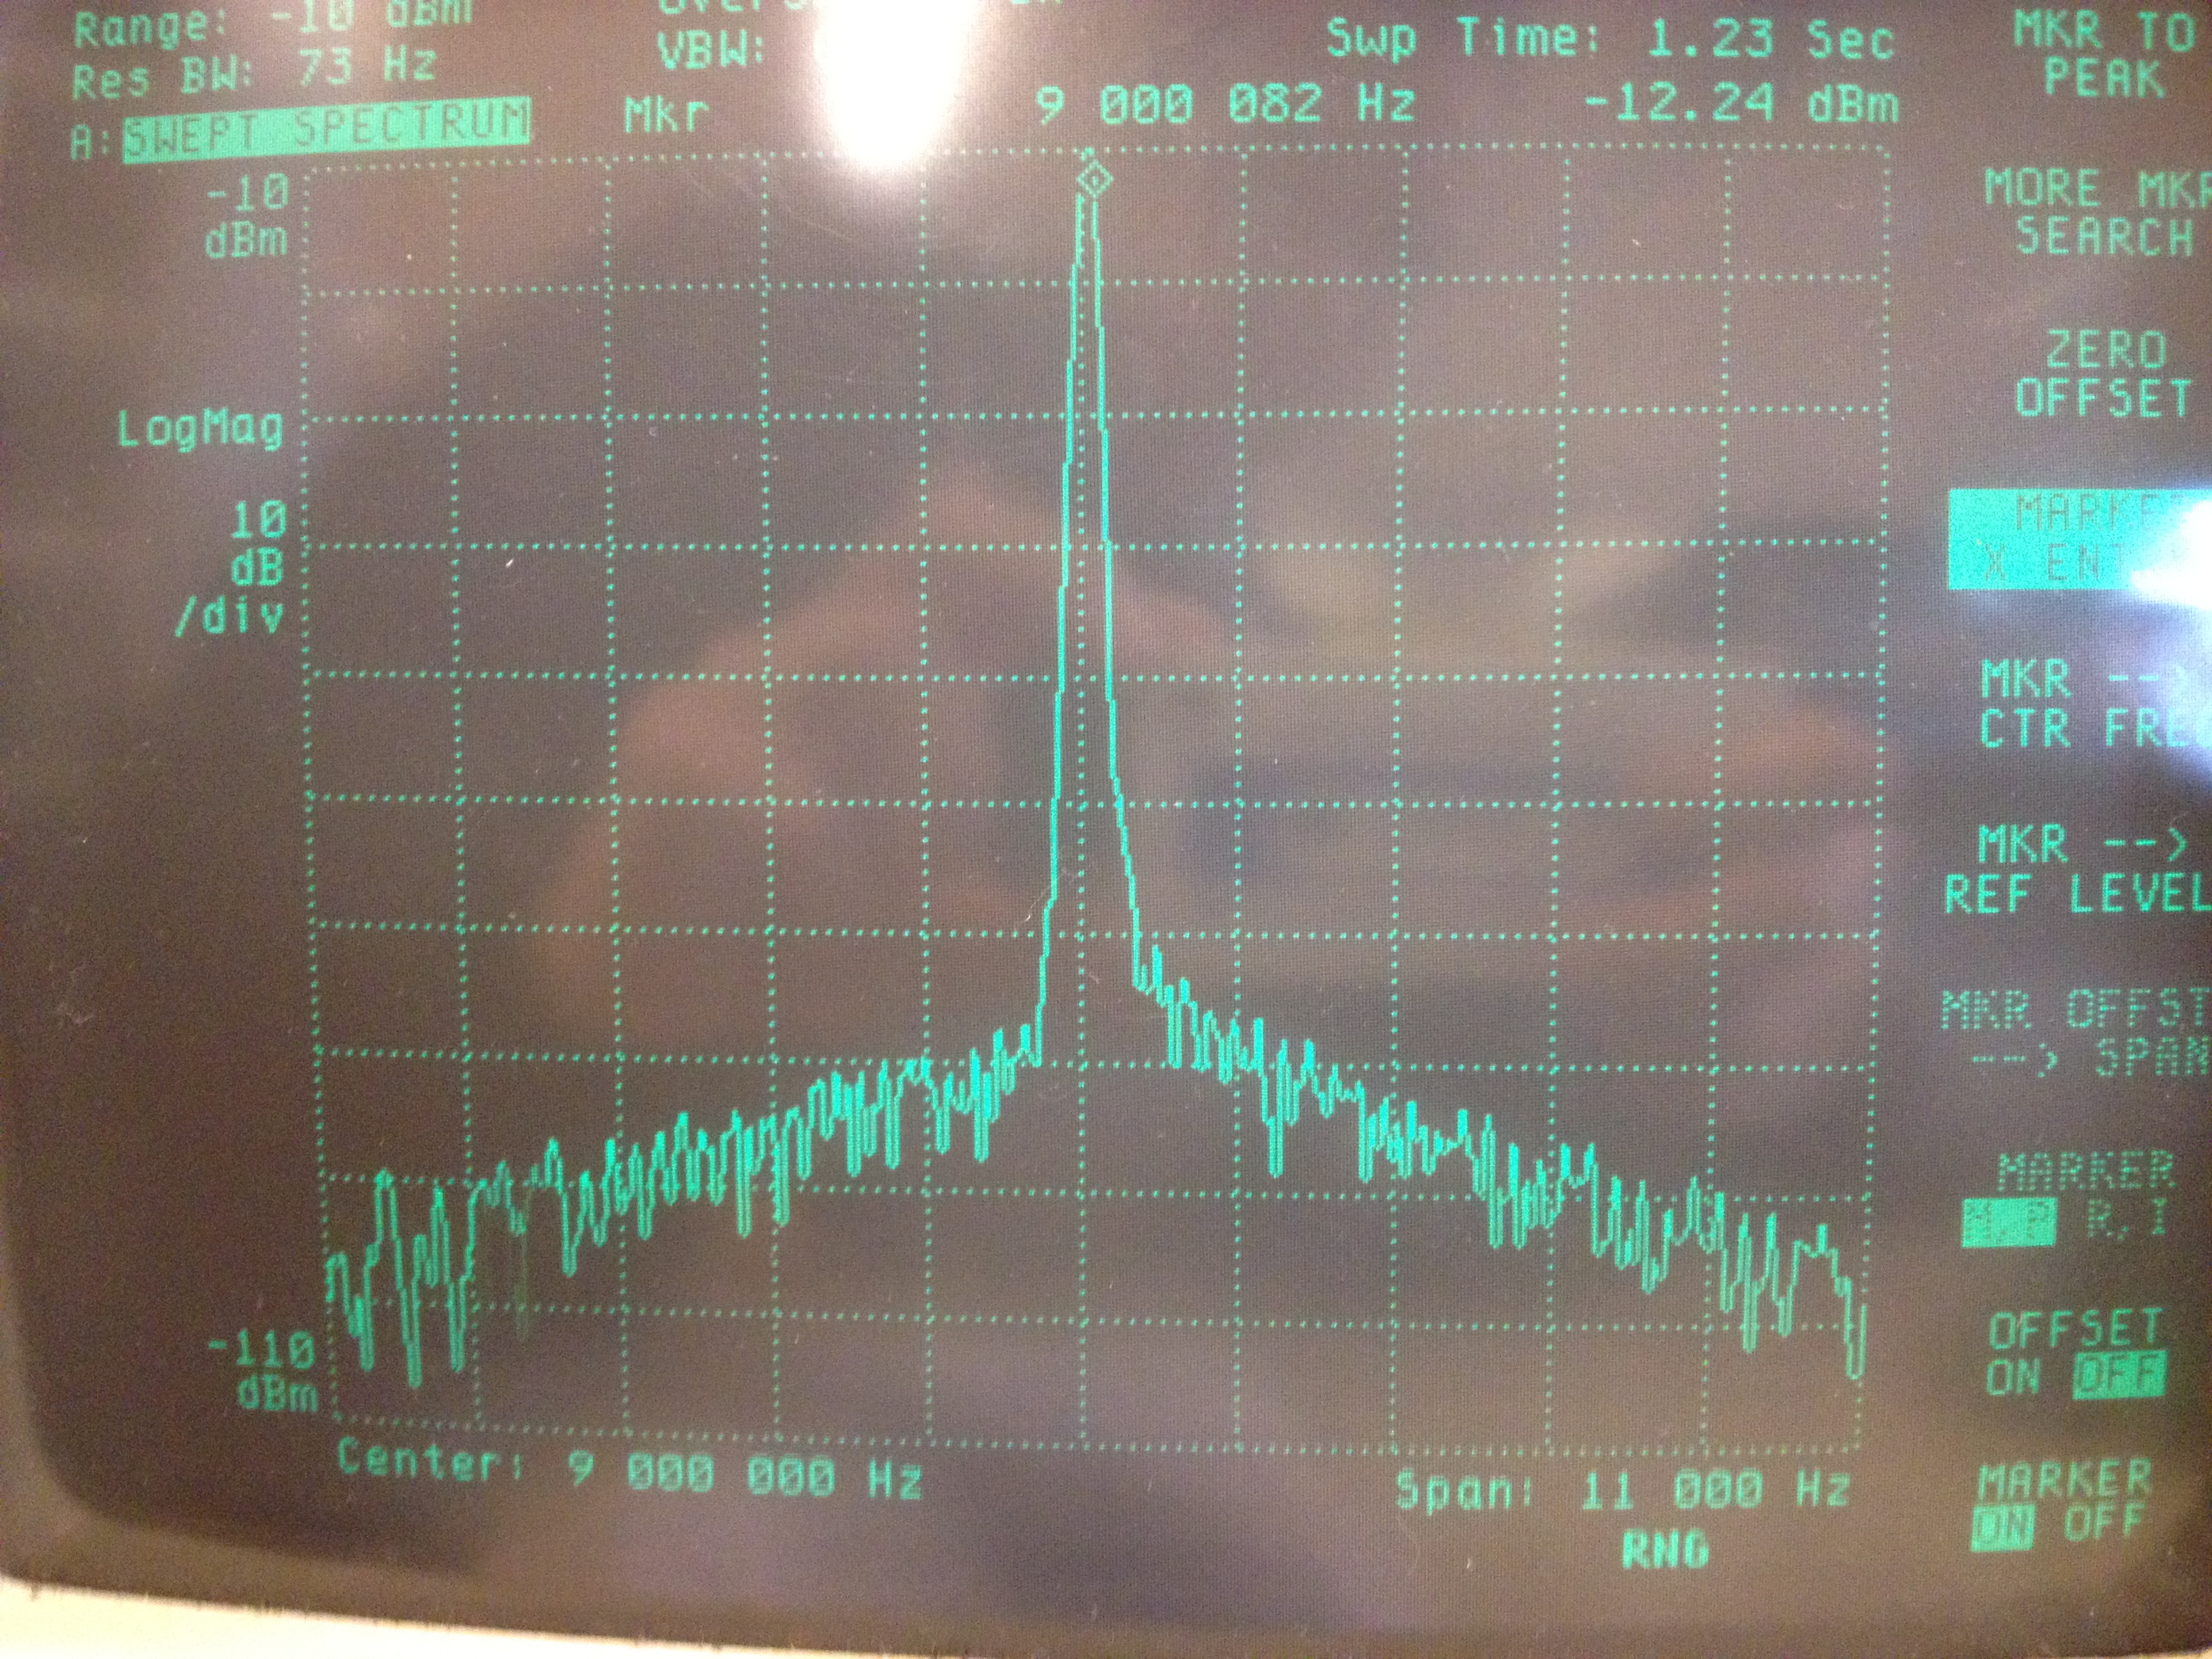
\includegraphics[width = 0.7\linewidth]{7_3_3_spectre9MHz.jpg}
\end{center}

\exsubpart{4}

Réglage de P41 : On constate que, lorsqu'on monte le curseur, la fréquence augmente. Augmenter le curseur revient à charger plus la sortie donc à diminuer le facteur de qualité du résonateur de sortie. Apparemment notre quartz à une fréquence propre un peu plus élevée que 9MHz mais le réglage à été établi de manière à ajuster la fréquence. Le fait de diminuer le facteur de qualité diminue l'influence du réglage sur la fréquence, d'où un rapprochement à la fréquence propre du quartz c'est à dire une augmentation.


\exsubpart{5,6}

Spectre de sortie de 1MHz à 100MHz :\\
\begin{center}
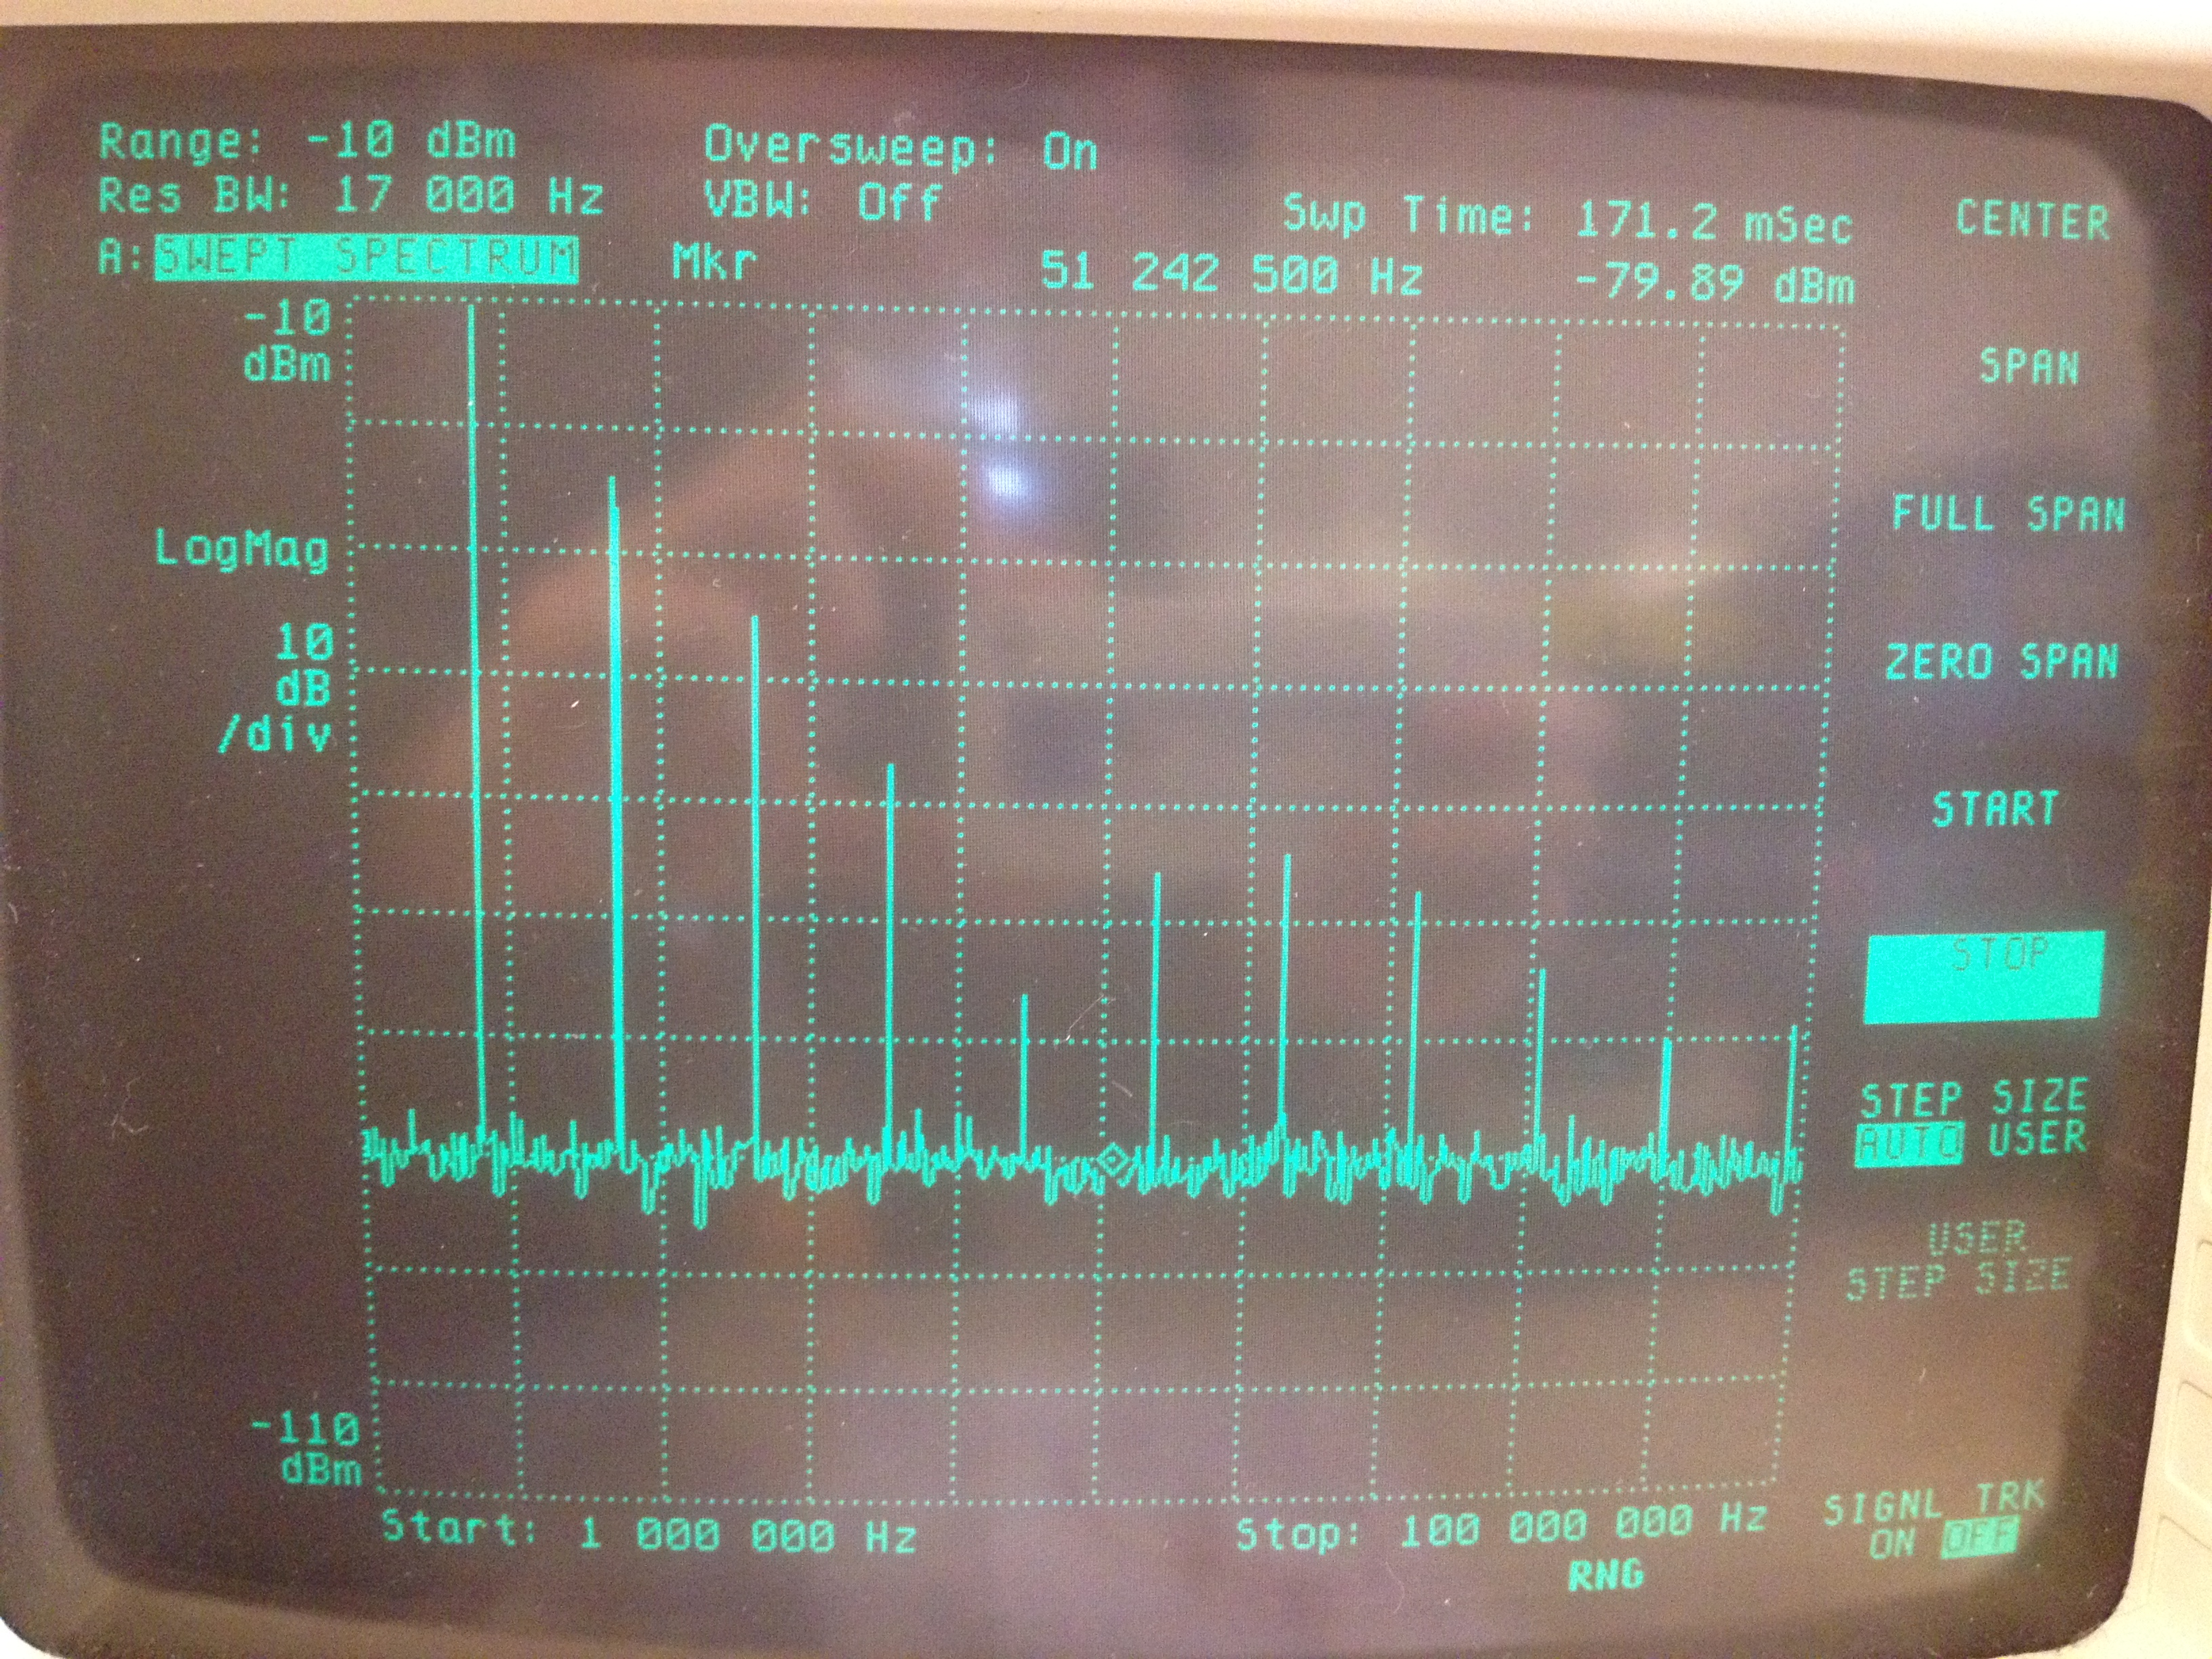
\includegraphics[width = 0.7\linewidth]{7_3_6_1MHz_100MHz.jpg}
\end{center}

On constate que le quartz à de nombreuses harmoniques, qui s'observent sur la sortie malgré le filtre de sortie $L_{41}$ et $C_{42}$. Sans l'effet de ce filtre, l'intensité de toutes les harmoniques serait probablement presque égal. Il est donc possible de faire osciller ce circuit à une autre fréquence avec le même quartz, en changeant les composants. On peut alors choisir une harmonique sur laquelle on vient s'accorder avec le quartz : Le filtre LC donne une grossière approximation de la région où les oscillations vont démarrer tandis que le quartz règle précisément la fréquence.


\section{Mélangeurs}

\subsection{Introduction}
Les mélangeurs sont des circuits qui permettent de multiplier deux signaux sinusoïdaux.
D'après la formule d'addition des sinus :
\begin{center}
$\sin(\omega_{1}\cdot t)\cdot \sin(\omega_{2}\cdot t) = \frac{1}{2}\cdot(\cos((\omega_{1} - \omega_{2})\cdot t) - cos((\omega_{1} + \omega_{2})\cdot t ) )$
\end{center}

Pour un montage idéal, nous avons donc une première composante fréquentielle en $\omega_{1} - \omega_{2}$ et une deuxième en $\omega_{1} + \omega_{2}$

Il est alors possible par filtrage d'éliminer l'une de ces deux composantes, typiquement $\omega_{1} - \omega_{2}$, afin de ne garder que la composante en $\omega_{1} + \omega_{2}$.\\

Ceci est utile pour réaliser plusieurs types de modulation et de démodulation.
\\
En pratique, la multiplication va présenter des non linéarités, nous aurons donc des harmoniques de $\omega_{1}$ et de $\omega_{2}$ en entrée du système.
Ainsi, nous avons des composantes à toutes les fréquences : $m \cdot \omega_{1} + n \cdot \omega_{2}$, $\forall m, n \in\bbZ$


\subsection{Mélangeur à circuit intégré NE602}

La multiplication des signaux IN1 et IN2 est faite par le circuit intégré NE602. 
Il s'agit d'un multiplicateur à 4 quadrants, c'est à dire que la sortie est valable pour toutes les combinaisons possibles des signes des tensions IN1 et IN2 (+, +), (+, -), (-, +) et (-, -).
Il n'y a donc aucunement besoin de polariser les entrées avec une composante continue, d'où un montage très simple.\\

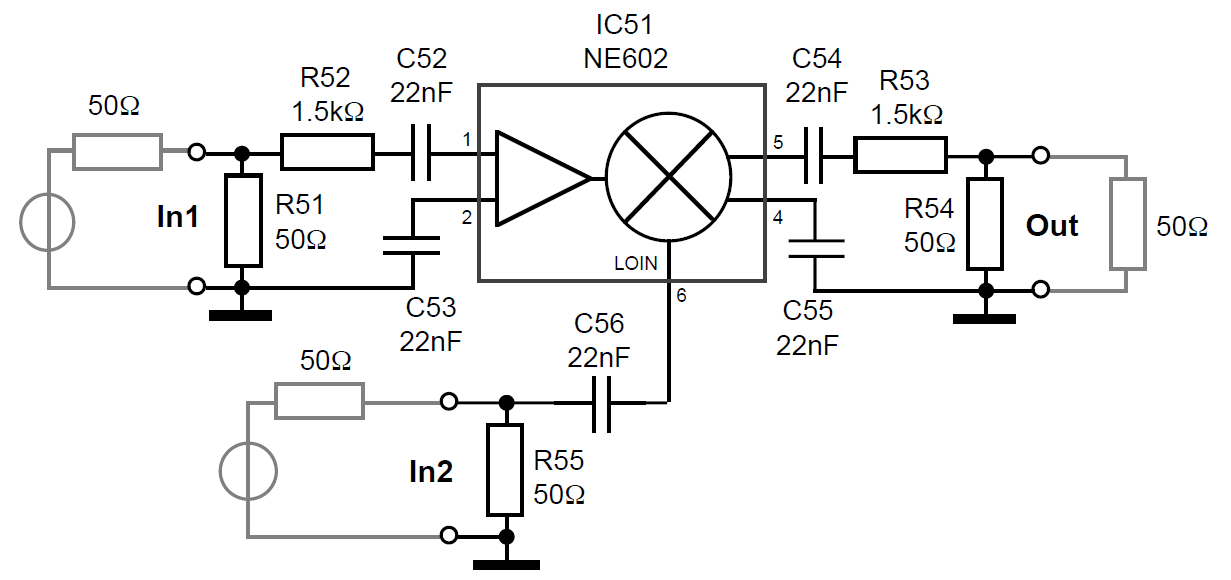
\includegraphics{shema_melangeur_gilbert.png}

\subsubsection{Questions et calculs}

\exsubpart{1}

L'impédance d'entrée sur l'amplificateur différentiel (broches 1 et 2) est d'environ $1.5k\Omega$ \footnote{Voir datasheet du composant NE602}. Idem pour les sorties sur les broches 4 et 5.
Les résistances $R_{51}$, $R_{52}$, $R_{53}$ et $R_{54}$ servent à adapter l'impédance du câble d'antenne $50\Omega$ vers le circuit intégré.\\

\begin{center}
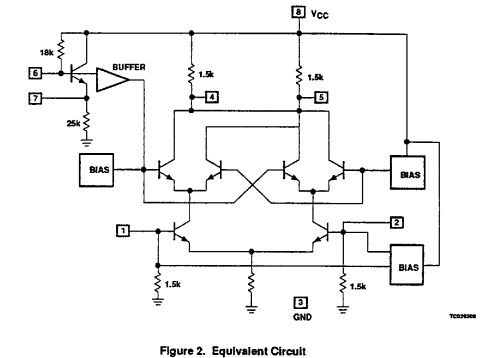
\includegraphics[width=0.85\linewidth]{shema_interne_ne602.png}
\end{center}

\exsubpart{2}

Le circuit a été prévu pour fabriquer un oscillateur avec les broches 6 et 7, cependant on n'utilise pas cette fonctionnalité, car nous avons notre propre oscillateur. L'amplitude doit être au moins de $200mV$ pour simuler un oscillateur local, qui n'est pas amplifié à l'intérieur du circuit, contrairement à l'entrée des broches 1 et 2 qui simule une antenne et qui est amplifiée en interne.

\subsubsection{Mesures}

\exsubpart{1}

Spectre de sortie :
\begin{center}
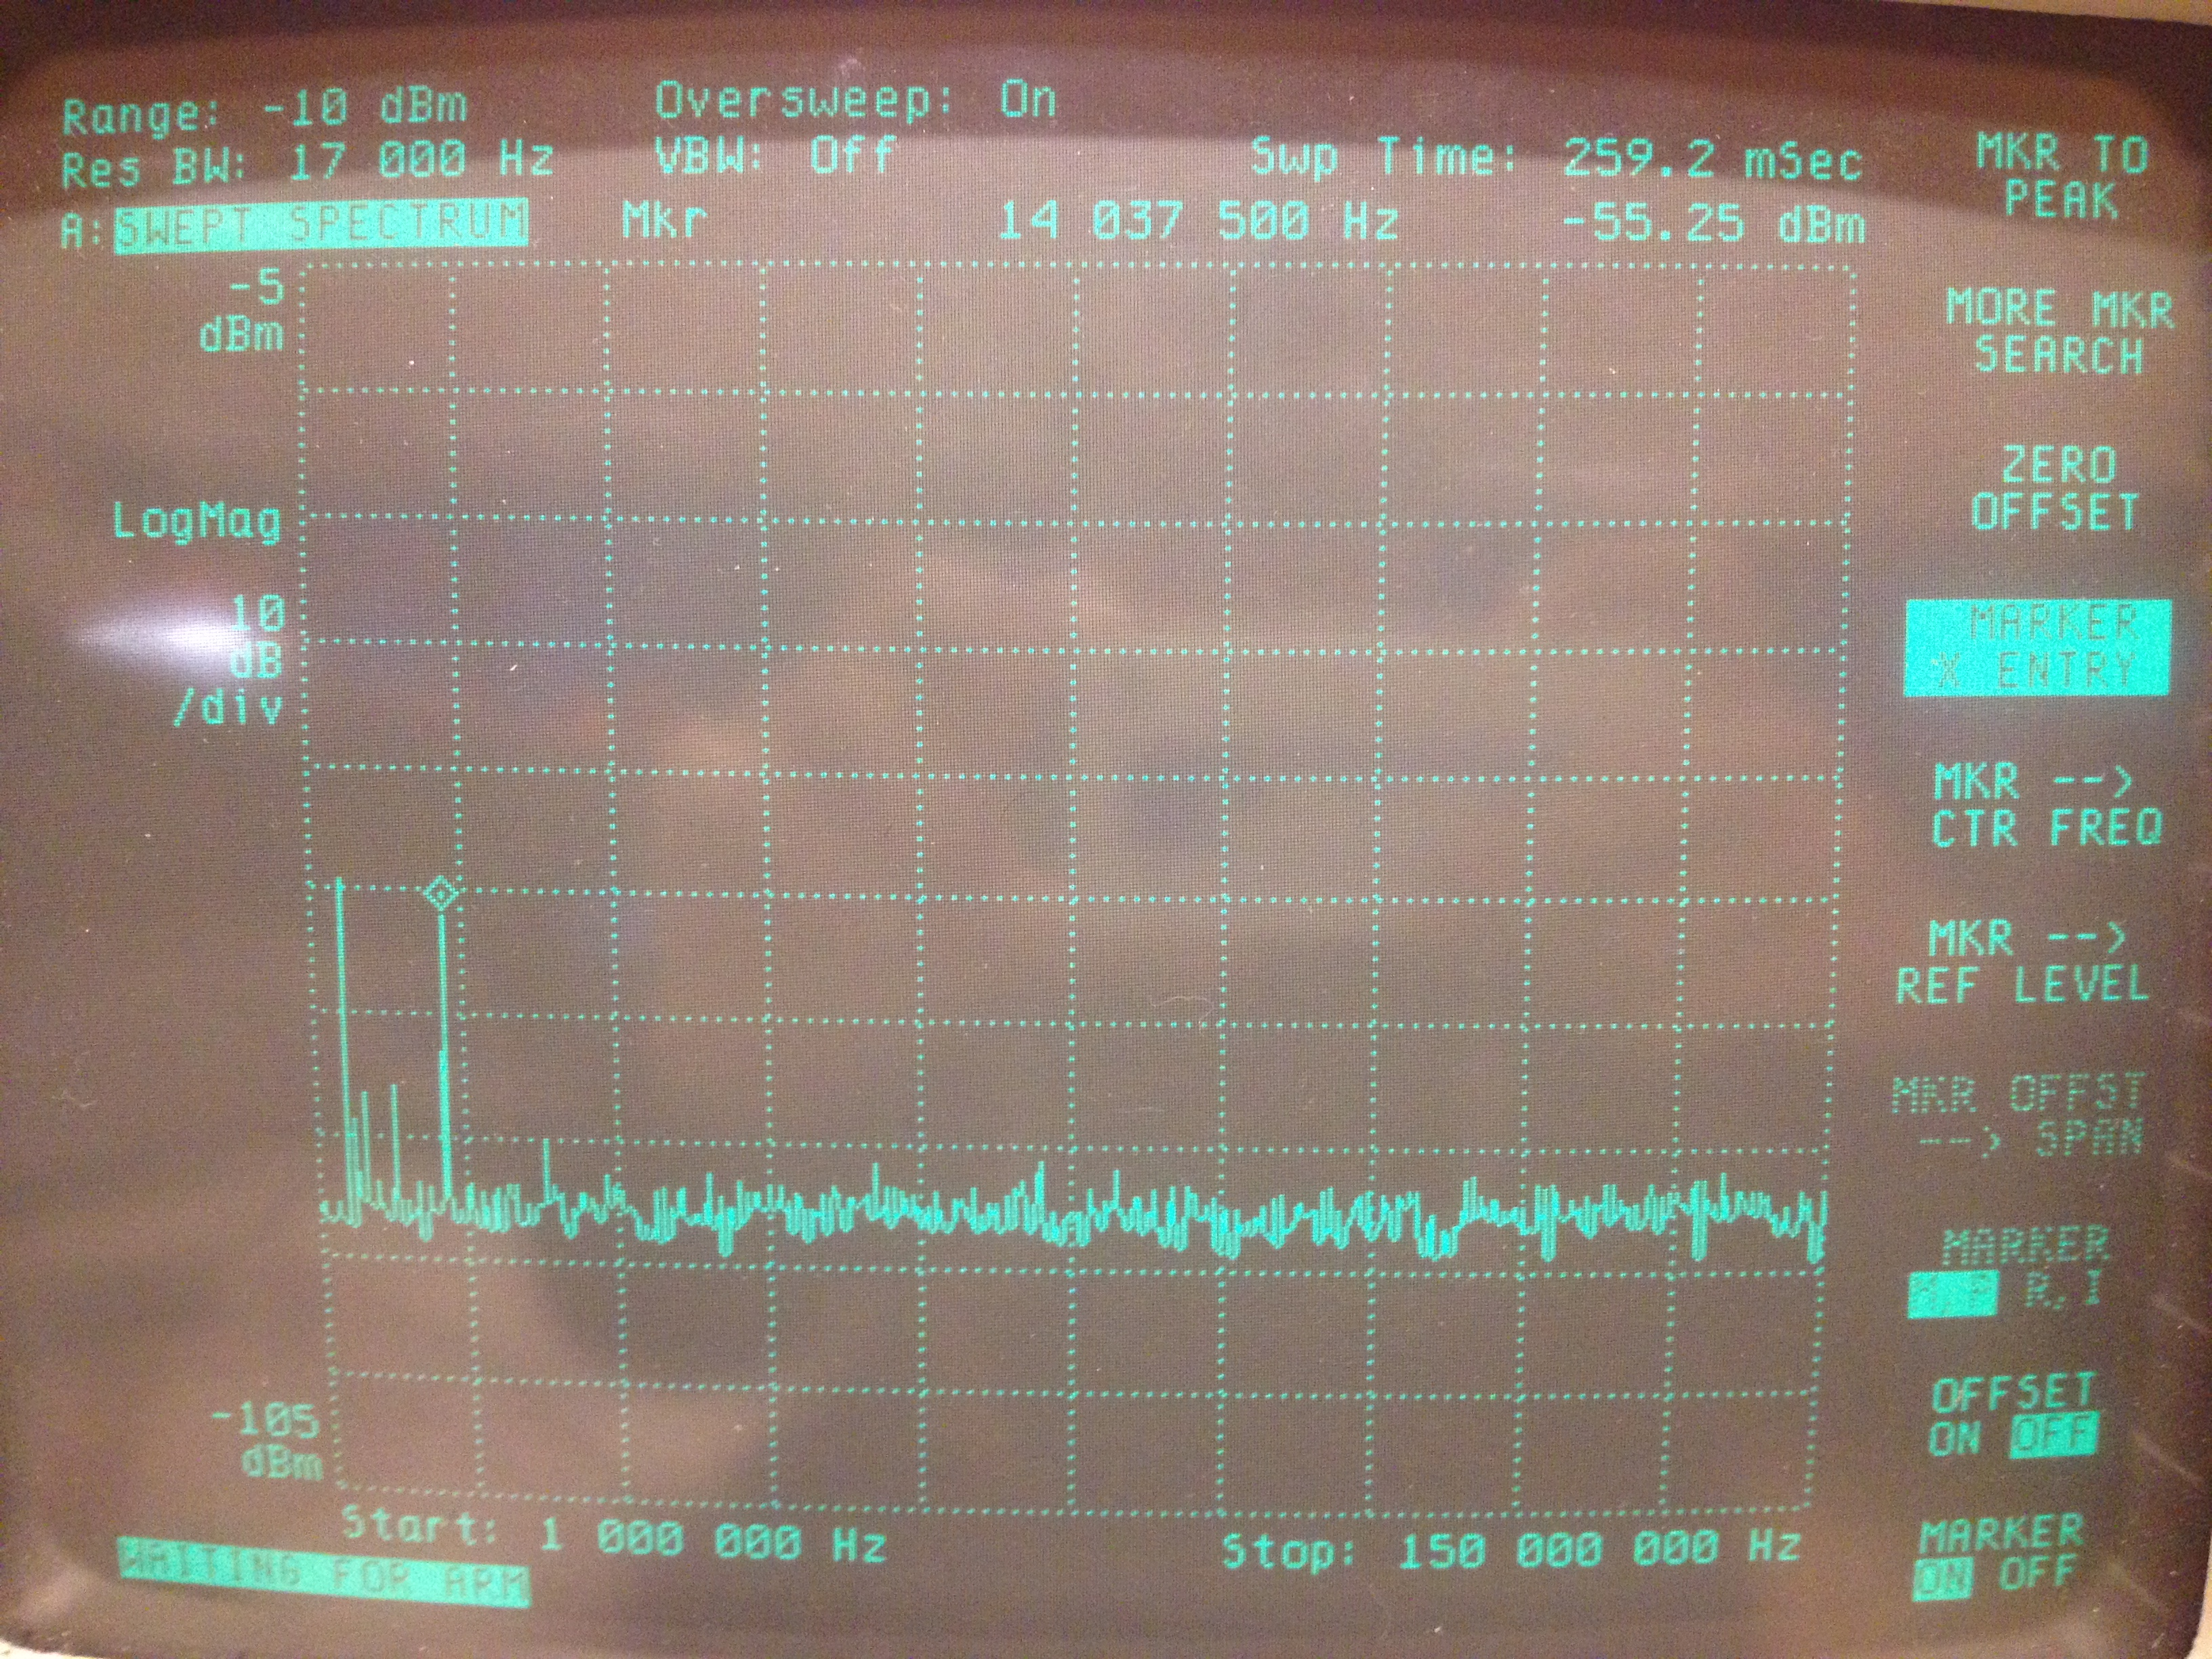
\includegraphics[width=0.7\linewidth]{8_3_1.jpg}
\end{center}

\exsubpart{2,3,4}
% Structurer en suivant les parties serait une bonne idée
% Expliquer le point d'interception du 3ème ordre ou dans les parties suivantes(antho)

\begin{itemize}

\item Gain de conversion : 13.3 dB
\item Point de compression de 1dB : -8.2 dBm
\item Point d'interception du 3ème ordre : 6.55 dBm
\end{itemize}

A noter qu'il y a une perte de puissance considérable à cause du changement d'impédance. On perd la moitié du signal d'entrée utile sur le diviseur formé par $R_{in}$ et $R_{51}$, soit $-6$ dB. On perd une grande partie de la puissance de sortie à cause du diviseur formé par $R_{53}$ et $R_{54}$, les pertes sont de :
\begin{center}
$Pertes = 20\cdot \log (\frac{R_{54} // R_{out}}{(R_{54} // R_{out})+R_{53}}) = 20\cdot \log{25}{25+1500}) \simeq -35.7$ dB
\end{center}

Nous avons donc, en réalité, 41.7 dB de plus que ce que nous indique l'appareil.

Voici le spectre de sortie d'un signal double ton d'amplitude $-8$ dBm (l'appareil voit $-35.7$ dB de moins, soit $-43.7$ dBm):\\
\begin{center}
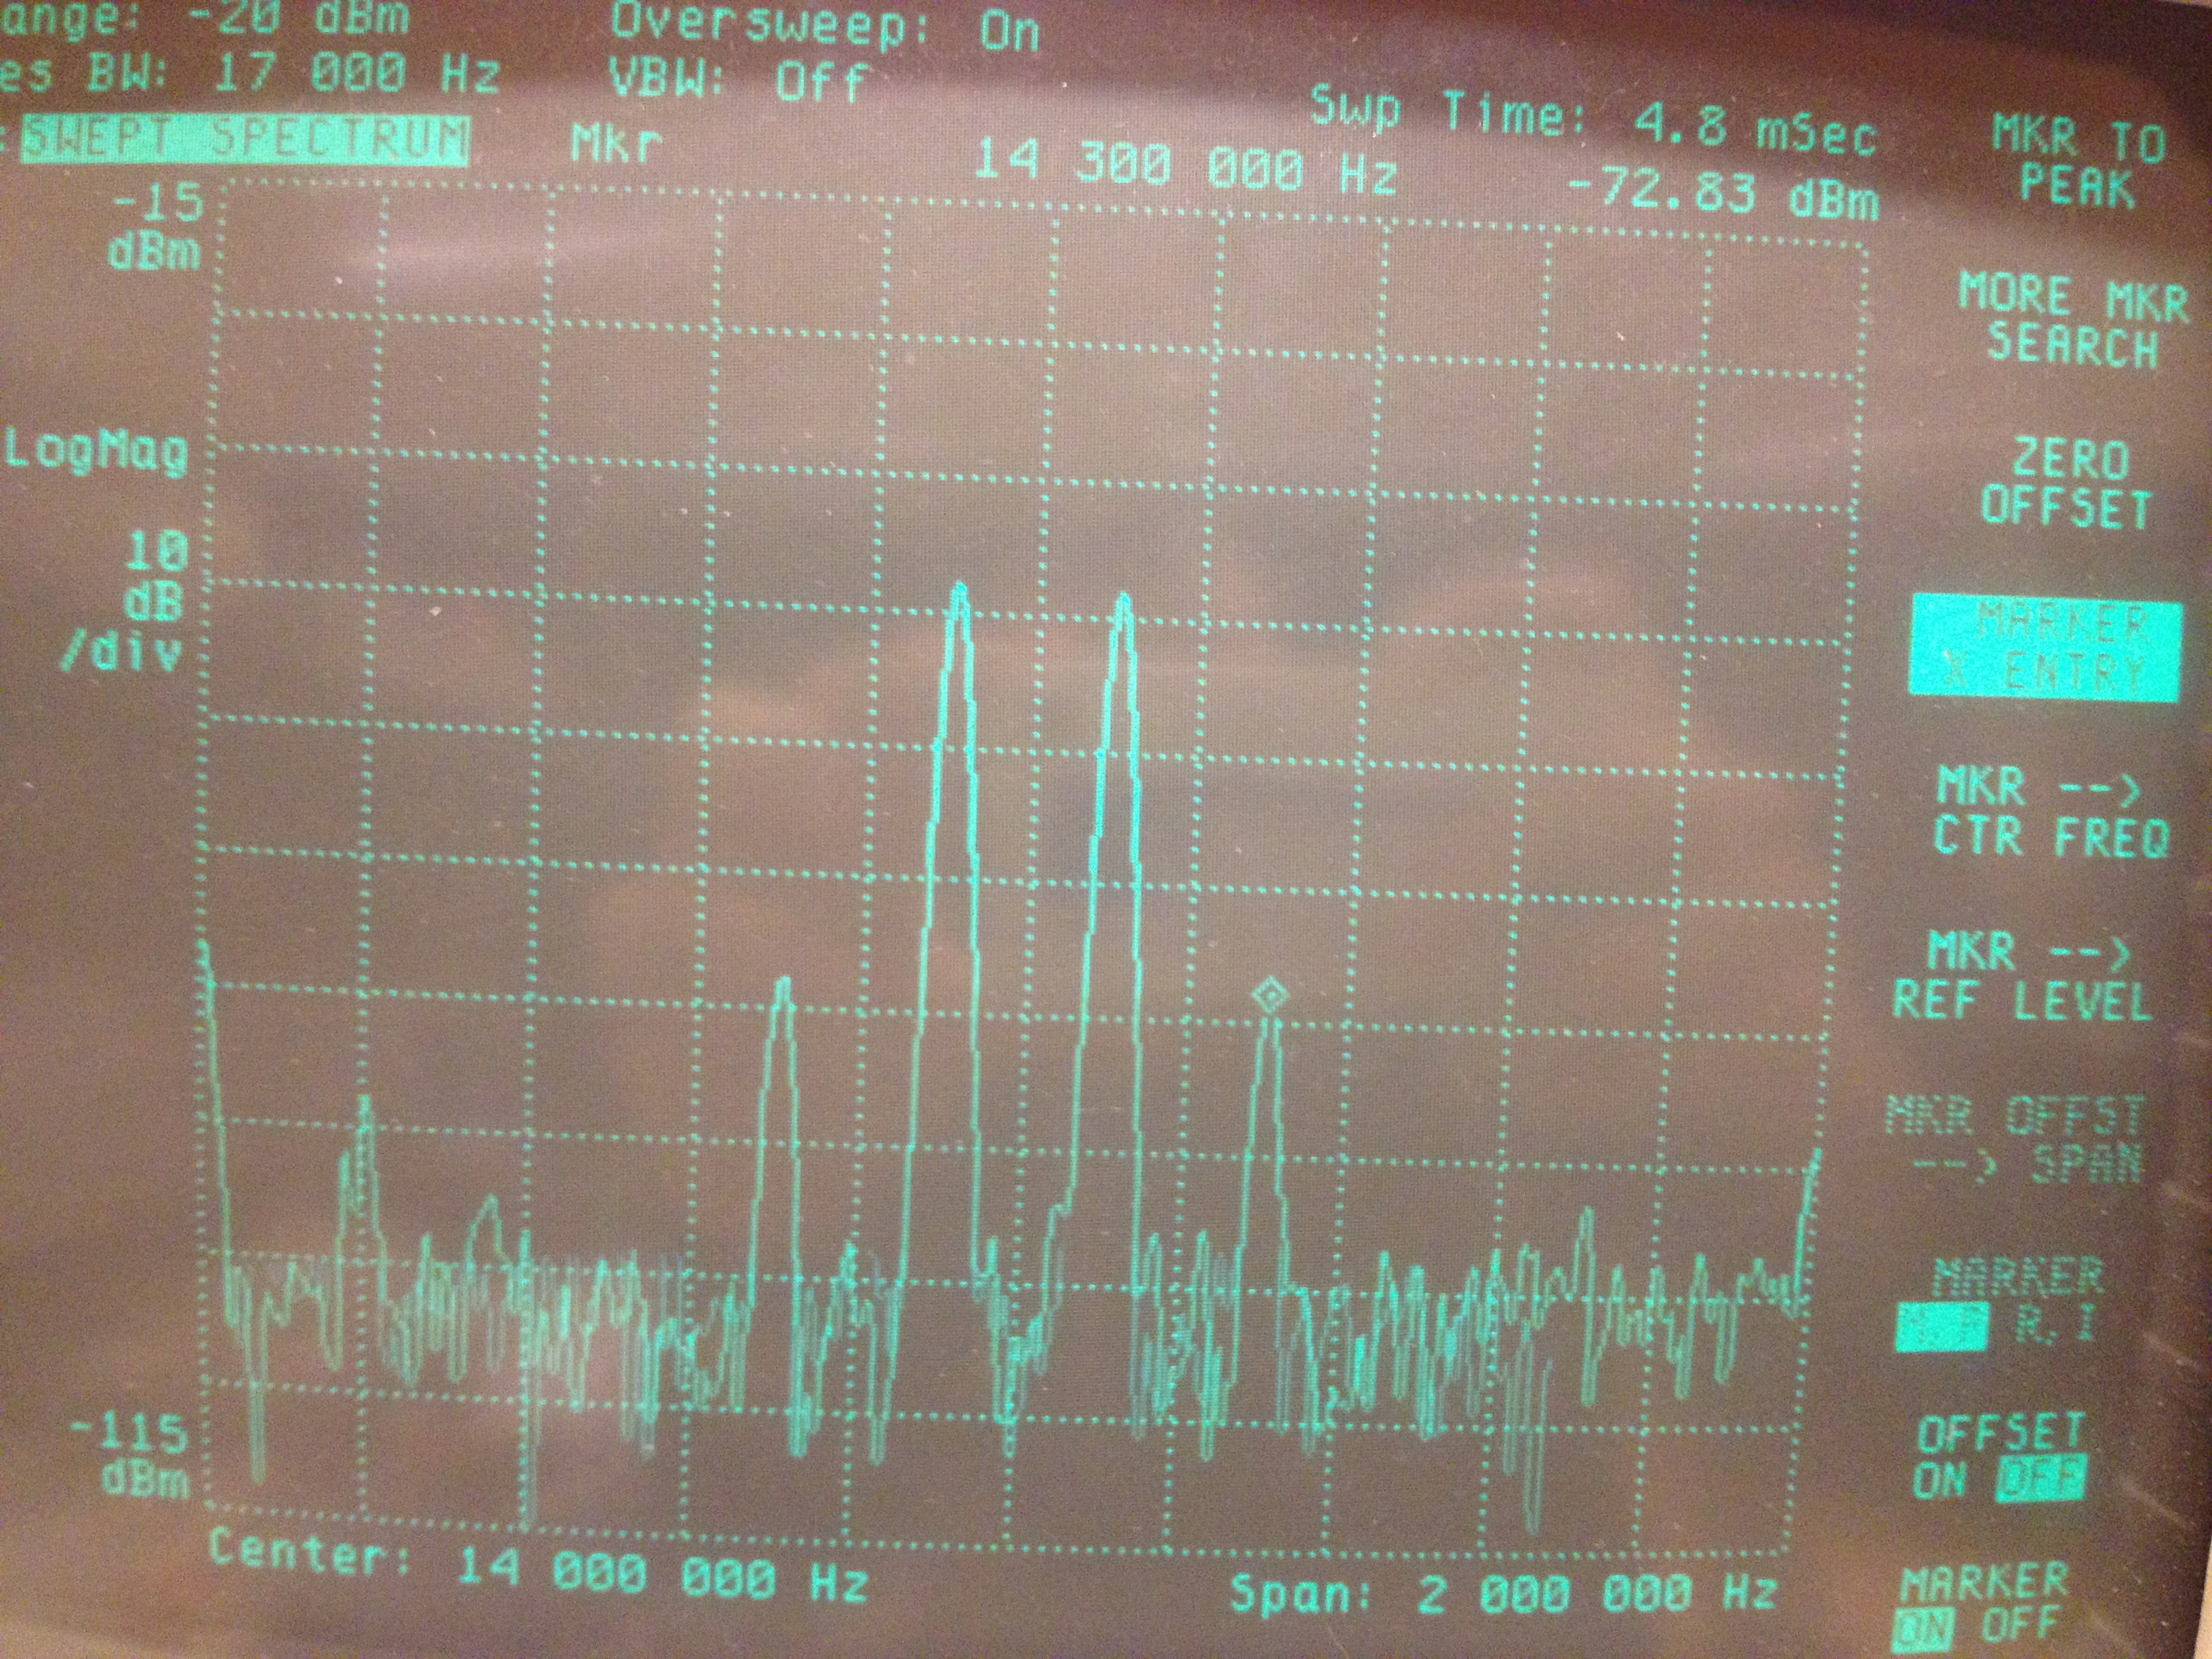
\includegraphics[width=0.7\linewidth]{8_3_4-8dbm.jpg}
\end{center}
Le pic de l'harmonique 3 est à $-72.8$ dBm pour l'appareil, c'est à dire en réalité $-72.8 + 35.7 = -37.1$ dBm.\\
On peut alors calculer le taux de distorsion d'inter-modulation d'ordre trois, c'est le point qui satisfait l'équation :
\begin{center}
$y = -37.1 + 3 \cdot (y+8) \Rightarrow y = 6.55$ dBm
\end{center}

%
% Parties d'Anthony, NON FINIE !
%
% To do :
%			- Expliquer le point d'interception d'ordre 3 et mettre les valeurs
%			- Identifier harmoniques (Jo?)
%			- Gain de conversion positif vers 10 dB...
%


\subsection{Le mélangeur doublement équilibré à diodes}

On considère le mélangeur doublement équilibré à diodes décrit Fig.~\ref{fig:schema_melangeur_doublediode}.

\begin{figure}[h!]
	\centering
	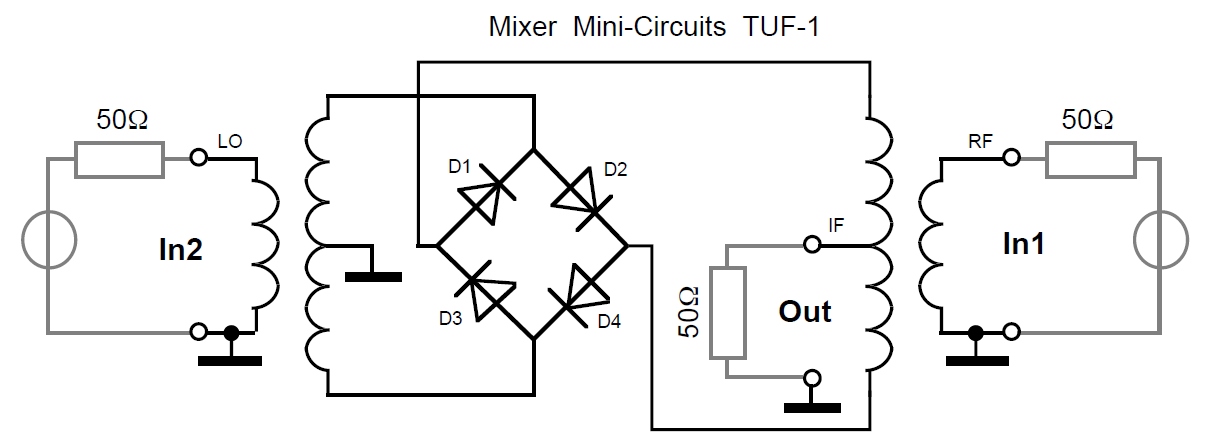
\includegraphics[width=.7\textwidth]{schema_melangeur_doublediode}
	\caption{Mélangeur doublement équilibré à diodes}
	\label{fig:schema_melangeur_doublediode}
\end{figure}

Ce mélangeur Schottky fonctionne comme un commutateur grâce à son pont de diode. Lors des alternances positives du signal d'entrée LO,  les D2 et D4 conduisent  et l'entrée RF se retrouve en phase  par rapport à la sortie IF. Lors des alternances négatives du signal LO, D1 et D3 conduisent et l'entrée RF est en inversion de phase. IF est donc le produit du signal RF par le signe du signal LO.

\subsubsection{Questions et calculs}

\exsubpart{1}

Chaque entrée (RF et LO) dispose d'une isolation galvanique avec la sortie IF. Ce type d'isolation permet de transmettre un signal entre 2 circuits électroniques qui n'ont pas forcément les mêmes niveaux de tensions et masses. On garantit ainsi une excellente isolation et indépendance entre les entrées et sortie dans notre cas.

\subsubsection{Mesures}

\exsubpart{1}

On applique sur IN2 qui est le Local Oscillator une sinusoïde à 5MHz d’amplitude  0.5 Veff et sur IN1, le signal à transmettre une sinusoïde à 9MHz d'amplitude 100 mVeff.
On observe le signal de sortie entre 1 et 150MHz afin d'avoir une vue d'ensemble.

\begin{figure}[h!]
	\centering
	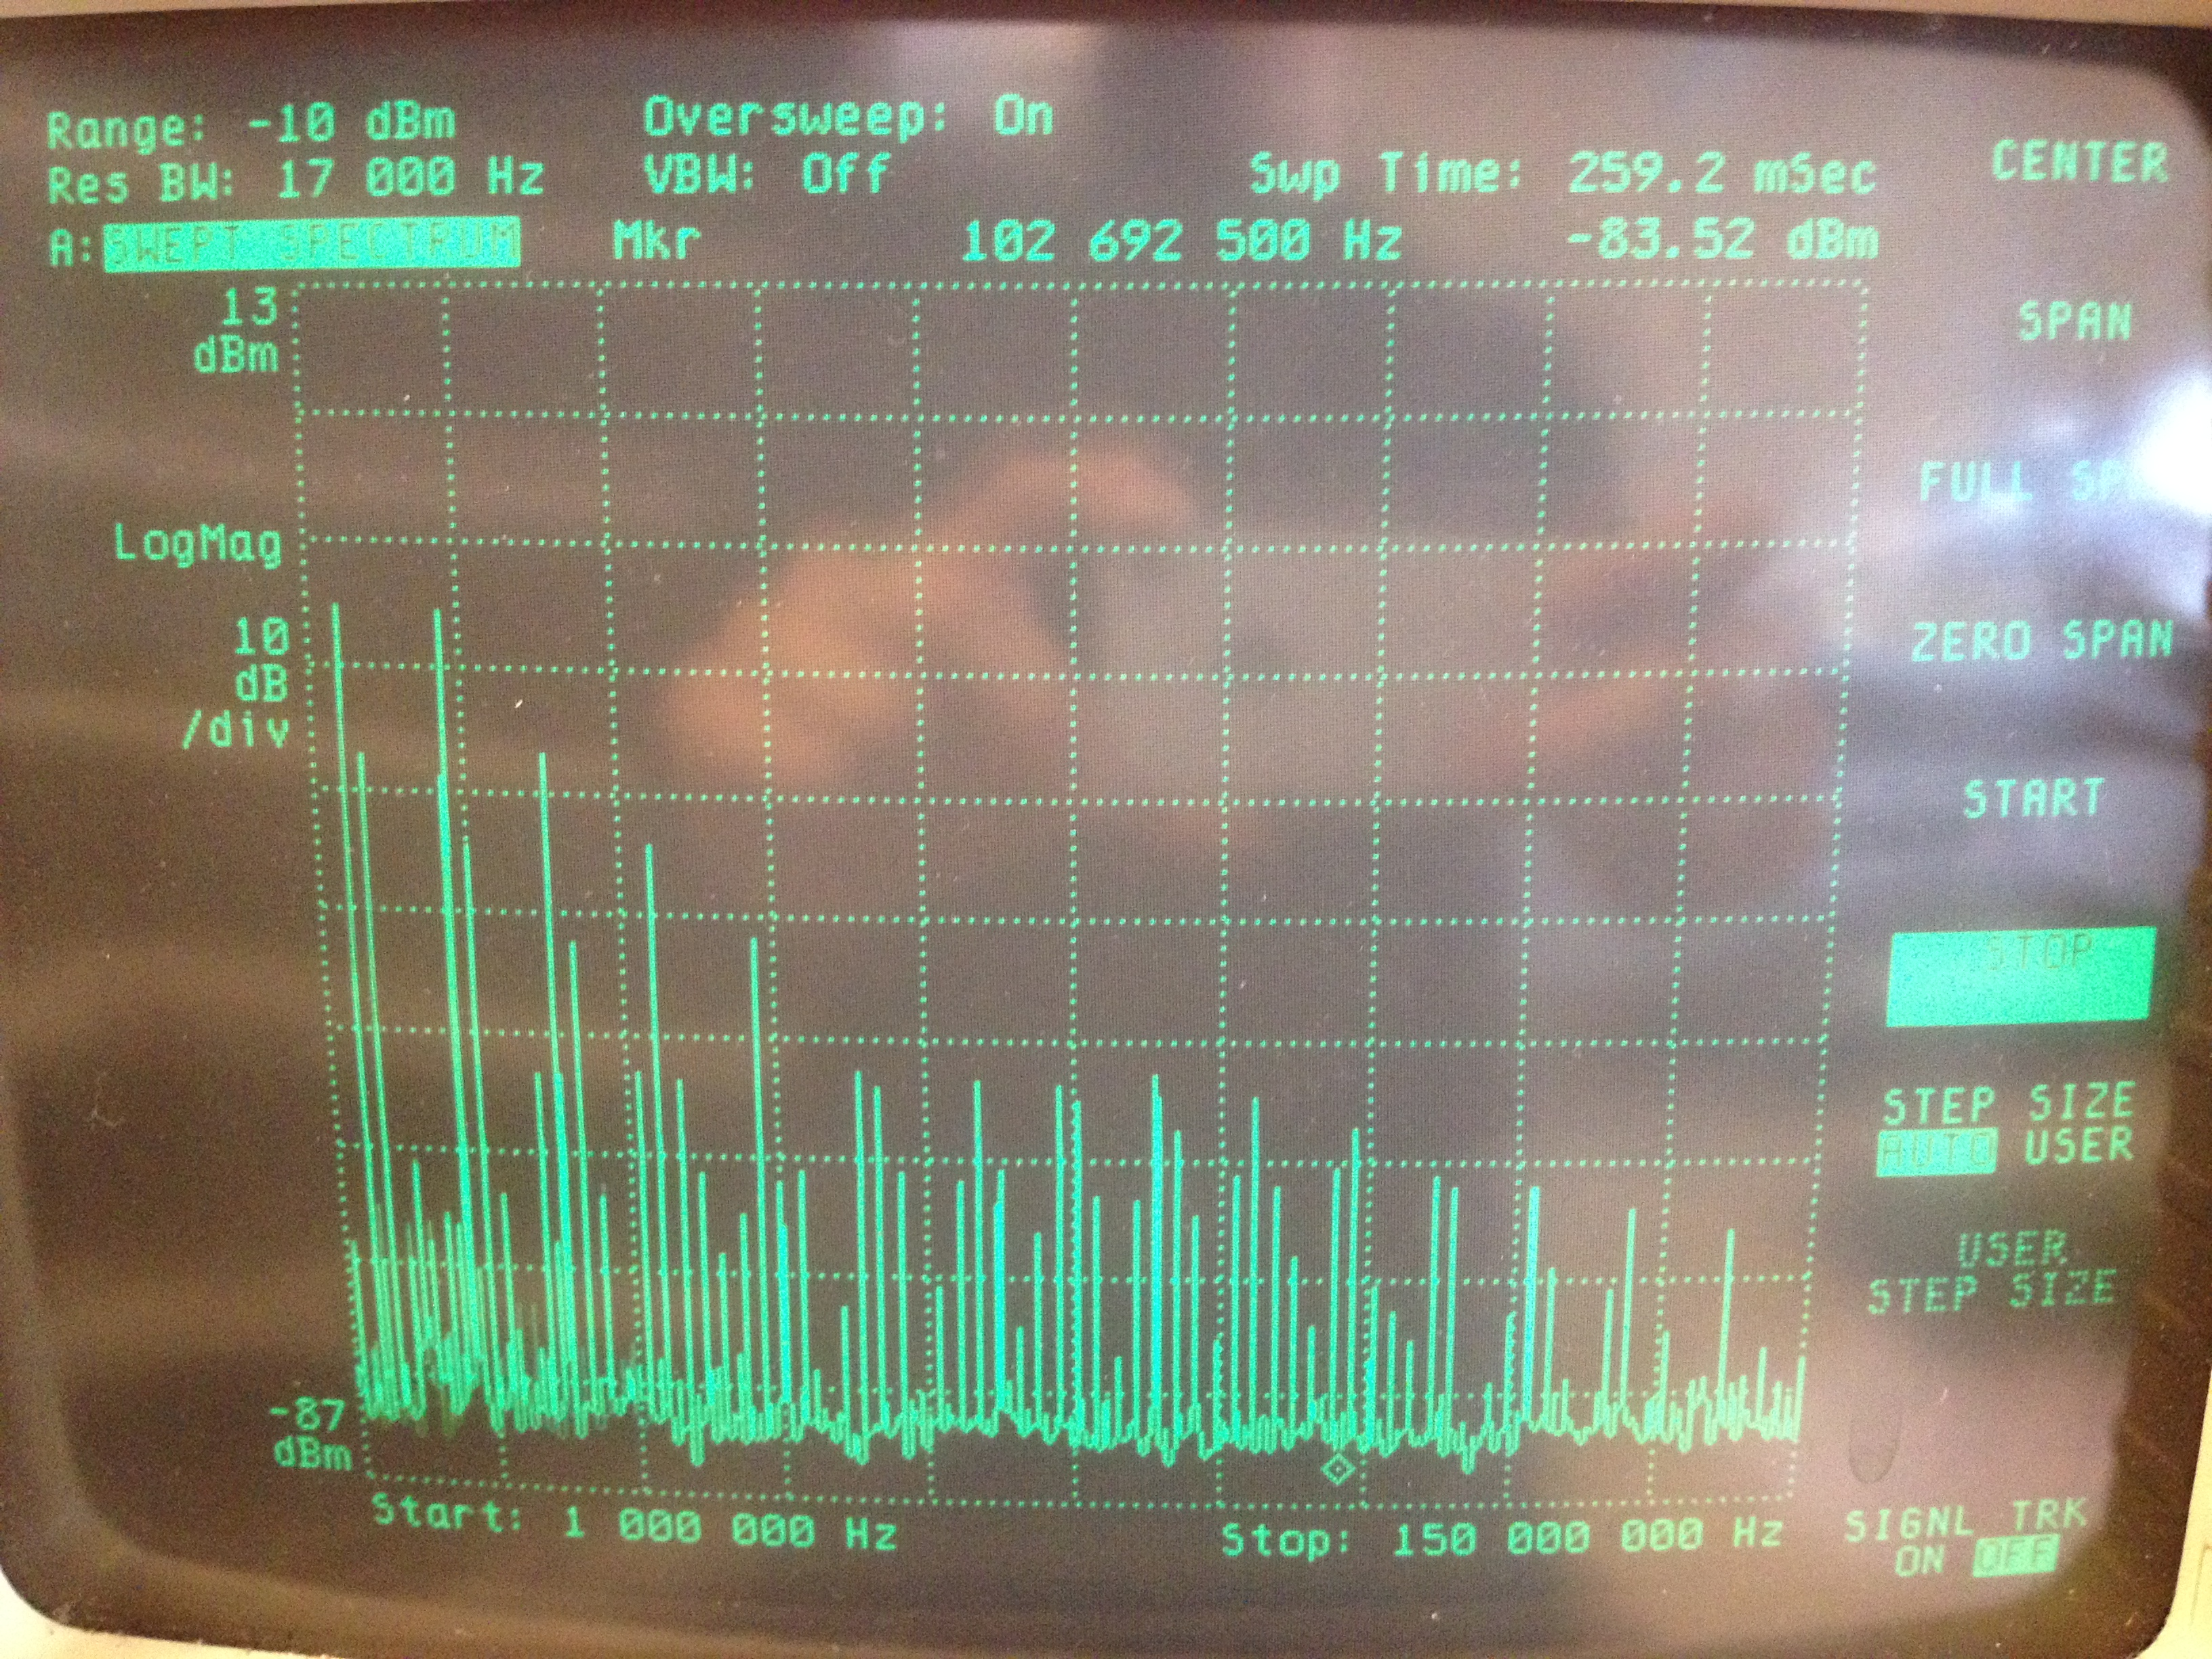
\includegraphics[width=.7\textwidth]{9_3_1}
	\caption{Réponse du mélangeur doublement équilibré à diodes de 1MHz à 100MHz}
	\label{fig:9_3_1}
\end{figure}


De nombreuses raies apparaissent, celles-ci sont en effet dues aux termes d'ordre supérieur à 1 de la multiplication.
%Identifier fréq raies ? fait à la partie de Jonathan ???

\exsubpart{2}

En observant de plus près, la zone fréquentielle résultat du mélange qui nous intéresse (autour de 14MHz), on parvient à calculer le gain de conversion.
L'amplitude en sortie à 14 MHz mesurée est de -12.5dBm avec un signal d'entrée HF de -7 dBm (0.5 Veff).
Le gain de conversion est de -5.5 dB.

\exsubpart{3}

On cherche à trouver le point de compression de 1dB. Pour cela, on augmente progressivement l'amplitude du signal d'entrée RF afin d'observer une différence de gain de 1dB avec le résultat de la question précédente.
Pour une amplitude d'entrée de 1dBm (0.250 Veff), la sortie à 14MHz a une amplitude de -5.5dBm, ce qui correspond à un gain de  conversion de -6.5 dB.

Le point de compression de 1 dB est donc à 1 dBm.

\exsubpart{4}

On injecte un signal double ton à l'aide d'un générateur de signaux supplémentaire et d'un sommateur passif de perte 6 dB.
On cherche tout d'abord à déterminer le taux de distorsion d'inter-modulation d'ordre trois.
En se plaçant à 10 dB en dessous du maximum pour notre signal d'entrée, on obtient le spectre suivant :

\begin{figure}[h!]
	\centering
	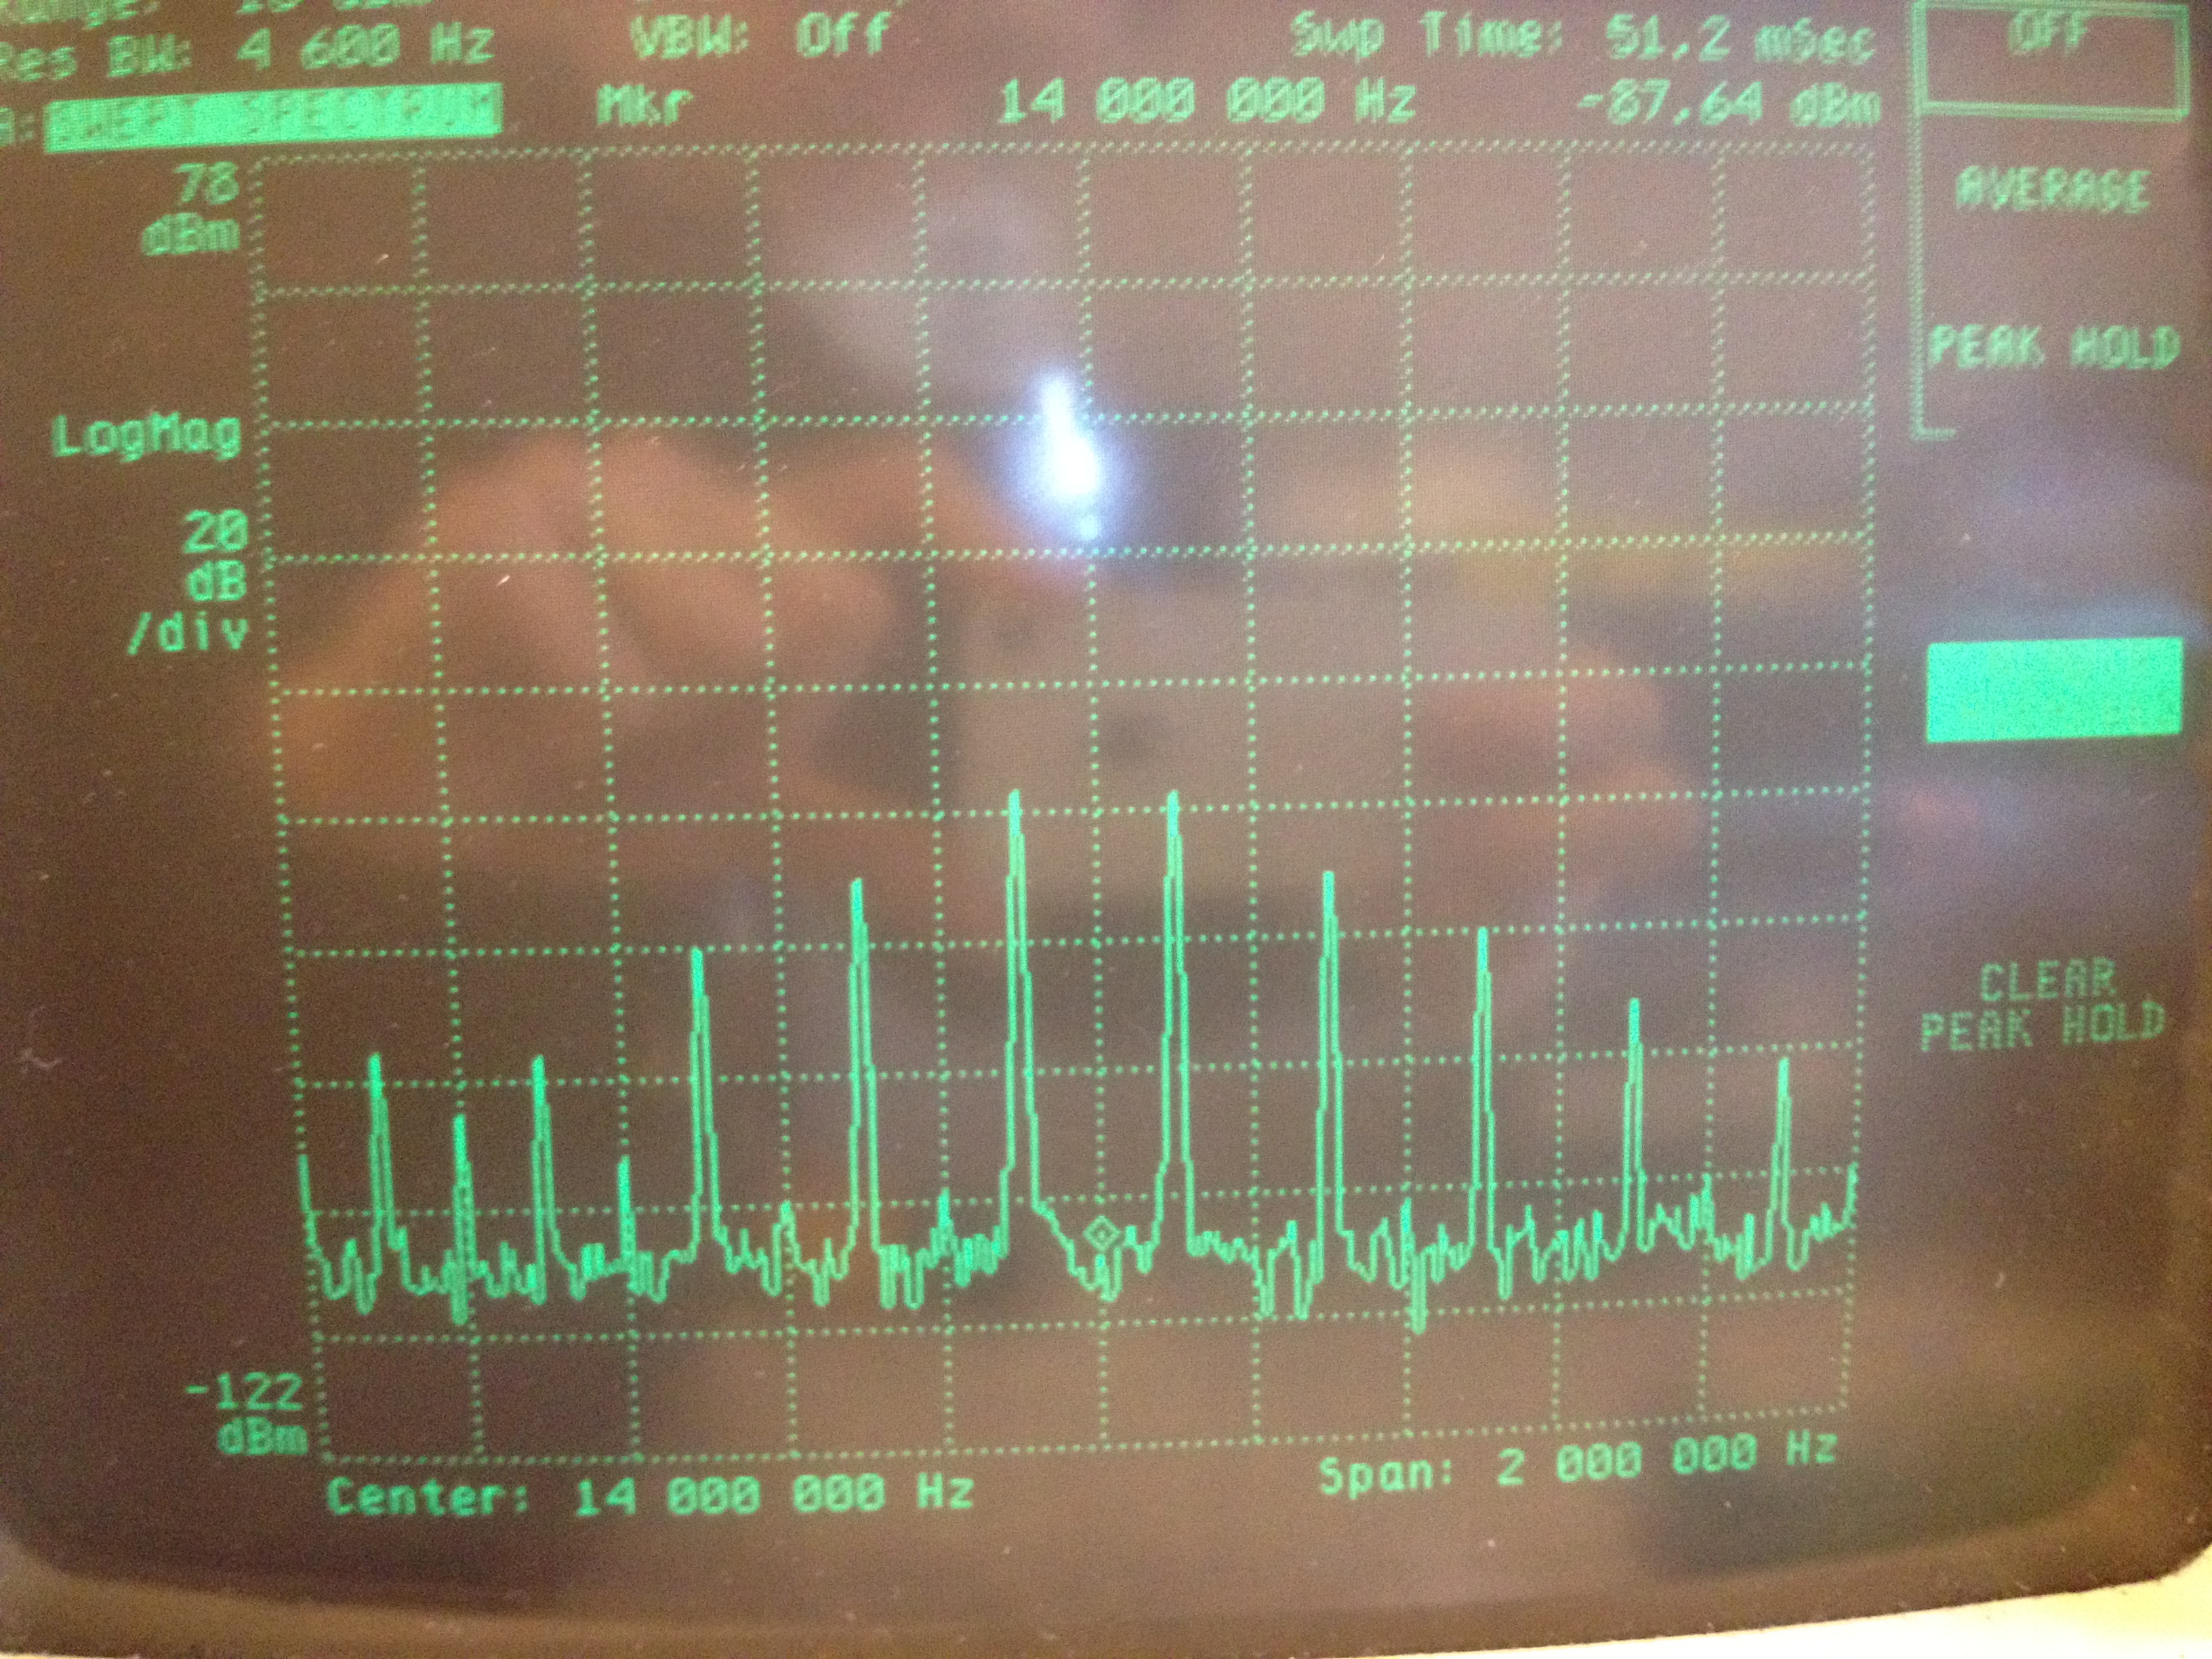
\includegraphics[width=.7\textwidth]{9_3_4}
	\caption{Spectre de la réponse à un signal double-ton à 8,9MHz et 9,1MHz}
	\label{fig:9_3_4}
\end{figure}
%(cheaté)
Le pic de l'harmonique de troisième ordre est de -32.3 dBm. C'est le taux de distorsion d'inter-modulation d'ordre 3 ($P_{IMR}$). A noter qu'on obtient ici directement l'amplitude du pic car l'isolation est galvanique sans étage d'adaptation qui nous font perdre de la puissance.
Ce taux nous permet de calculer directement le point d'interception d'ordre 3 (OIP3) correspondant au croisement entre les approximations linéaires de la fondamentale et de l'harmonique d'ordre 3 comme représenté Fig.~\ref{fig:schema_melangeur_mosdoublegate}.

\begin{figure}[h!]
	\centering
	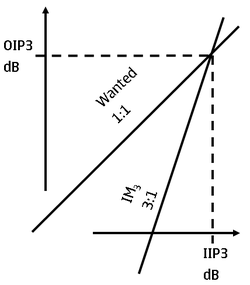
\includegraphics[width=.7\textwidth]{OIP3}
	\caption{Détermination du point d'interception d'ordre 3}
	\label{fig:OIP3}
\end{figure}

On a donc la formule suivante : $OIP3=L_{in}+G_{dB}-\frac{P_{IMR}}{2}$
Avec Lin= signal d'entrée en dBm = 1 ici, $G_{dB}$ le gain de conversion calculé à la question 2).
%
%------------------------------------------------------------------------------------------------------------------
Le point d'interception du troisième ordre est donc de ???
%------------------------------------------------------------------------------------------------------------------
 
\exsubpart{5}

On mesure l'isolation de l'entrée In2 (LO) vers In1 (RF) en chargeant la sortie avec une résistance de 50 $\Omega$ (50.47 exactement).
L'entrée IN2 (LO) est observée à l'analyseur de spectre, l'amplitude à la fréquence de 9MHz est de -62.82 dBm.

\begin{figure}[h!]
	\centering
	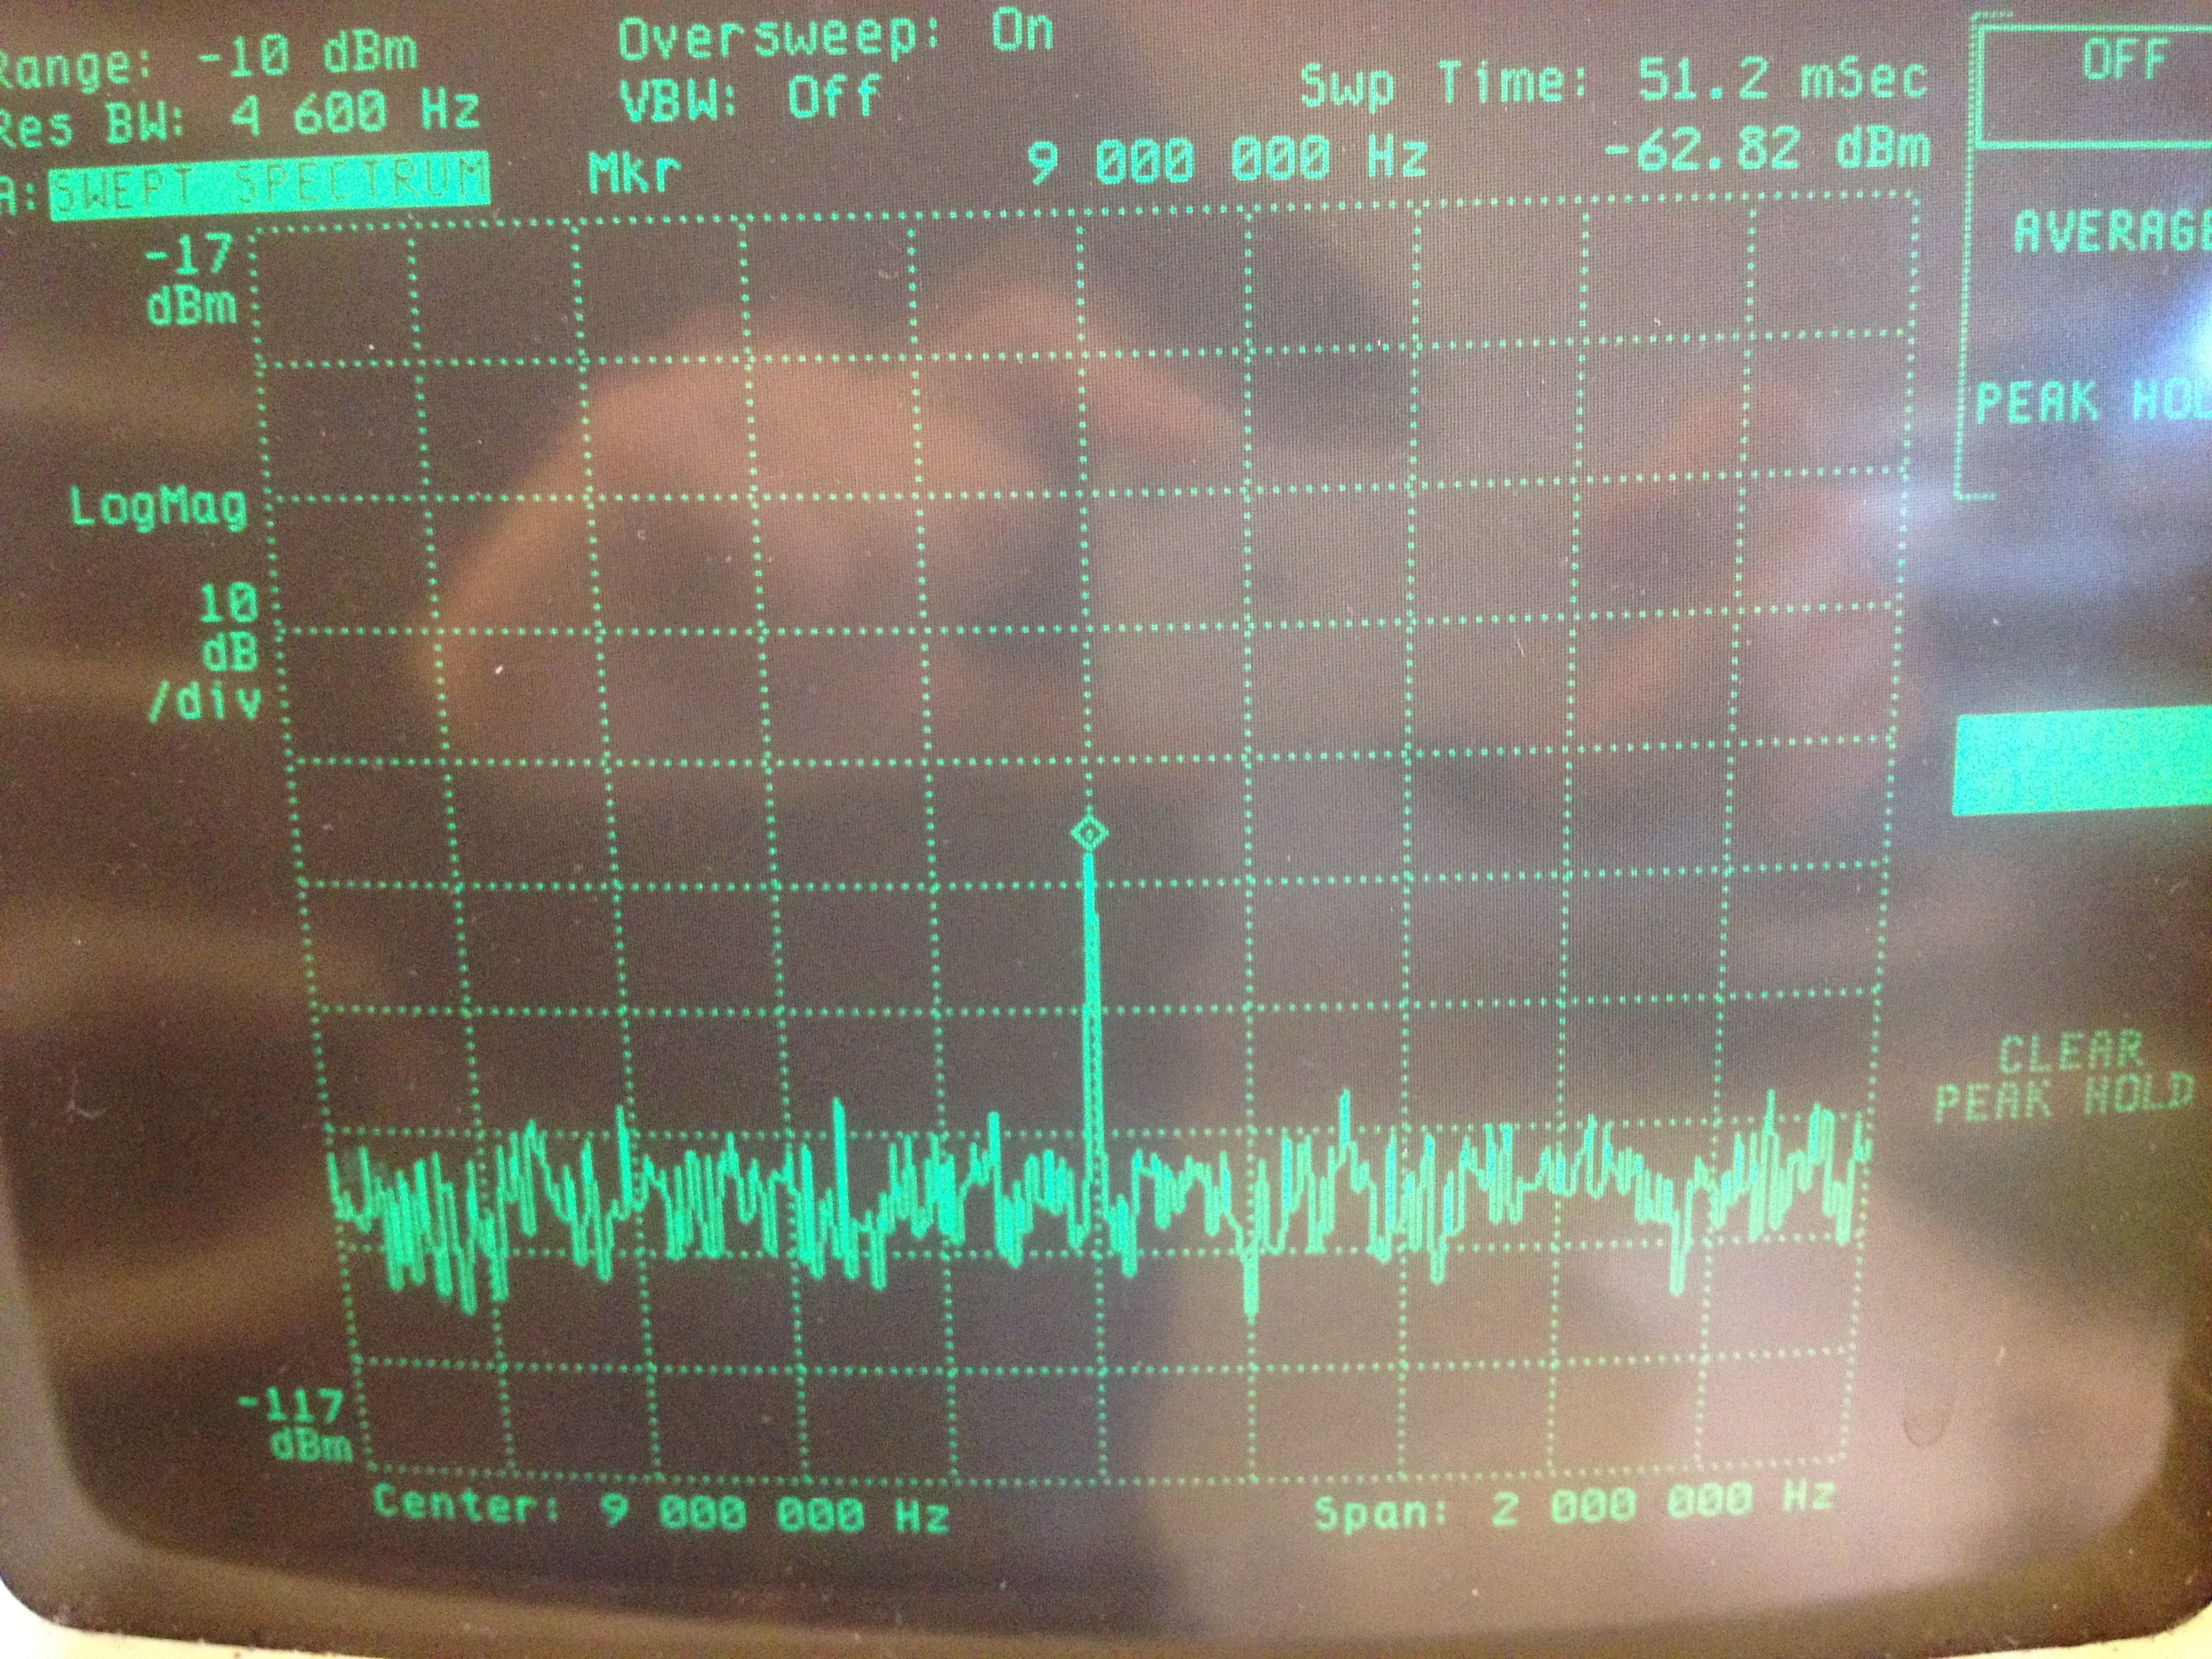
\includegraphics[width=.7\textwidth]{9_3_5}
	\caption{Isolation de l'entrée IN2 vers IN1}
	\label{fig:9_3_5}
\end{figure}

En enlevant le gain du signal d'entrée IN1 (HF), on obtient un gain et isolation de -67.5 dB, ce qui est correct.


\subsection{Le mélangeur à « MOS double-gate »}

On s'intéresse maintenant à un autre mélangeur, celui-ci comporte un transistor MOS à double grille comme décrit Fig.~\ref{fig:schema_melangeur_mosdoublegate}.

\begin{figure}[h!]
	\centering
	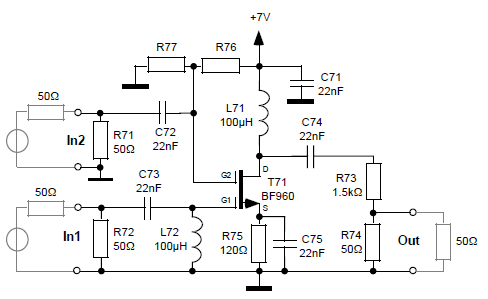
\includegraphics[width=.7\textwidth]{schema_melangeur_mosdoublegate}
	\caption{Mélangeur à « MOS double-gate »}
	\label{fig:schema_melangeur_mosdoublegate}
\end{figure}

Ces deux grilles sont très utiles et permettent au courant de drain d'être contrôlé par chacune des grilles. Dans notre cas, la grille G1 est légèrement polarisée négativement par rapport à la source, elle est reliée à l'entrée In1, alors que G2 est polarisée positivement grâce au pont diviseur de tension lié à VDD et réalisé par les résistances R76 et R77. Elle est reliée à In2.
Le signal In2 (LO) a une amplitude importante et va ainsi faire fortement varier le courant de drain grâce à G2. Le signal In1 (RF) d'une amplitude plus faible, va quand même faire varier le courant de drain du transistor mais le gain d'entrée G1 sera modulé par celui de G2. D'où l'appellation « modulateur d'amplitude » et l'effet de mélange.
On retrouve les adaptations d'impédance vers du 50 ohms nécessaires aux appareils de mesures.


\subsubsection{Questions et calculs}

\exsubpart{1}

On veut une tension de repos de 1V sur G2.
Les résistances $R_{76}$ et $R_{77}$ réalisent un pont diviseur de tension au potentiel de G2, on a donc :
\begin{equation*}
V_{G2}=1V={R_{77}}{(R_{77}+R_{76})}V_{dd}
\end{equation*}
On choisit donc :
\begin{itemize}
\item $R_{76}= 3.3 k \Omega$
\item $R_{77}= 560 \Omega$
\end{itemize}

\exsubpart{2}

$L_{72}$ permet de fixer la composante DC à G1 à la masse. On peut ainsi polariser le transistor comme on le souhaite, négativement dans notre cas. L'absence de cette inductance ne permet pas de contrôler la polarisation du transistor et le signal RF ne serait plus intégralement transmis.

\subsubsection{Mesures}

\exsubpart{1}

On applique sur IN2 qui est le Local Oscillator une sinusoïde à 5MHz d'amplitude  1 Veff  et sur IN1, le signal à transmettre une sinusoïde à 9MHz d'amplitude 10 mVeff.
On observe le signal de sortie entre 1 et 150MHz afin d'avoir une vue d'ensemble.
\begin{figure}[h!]
	\centering
	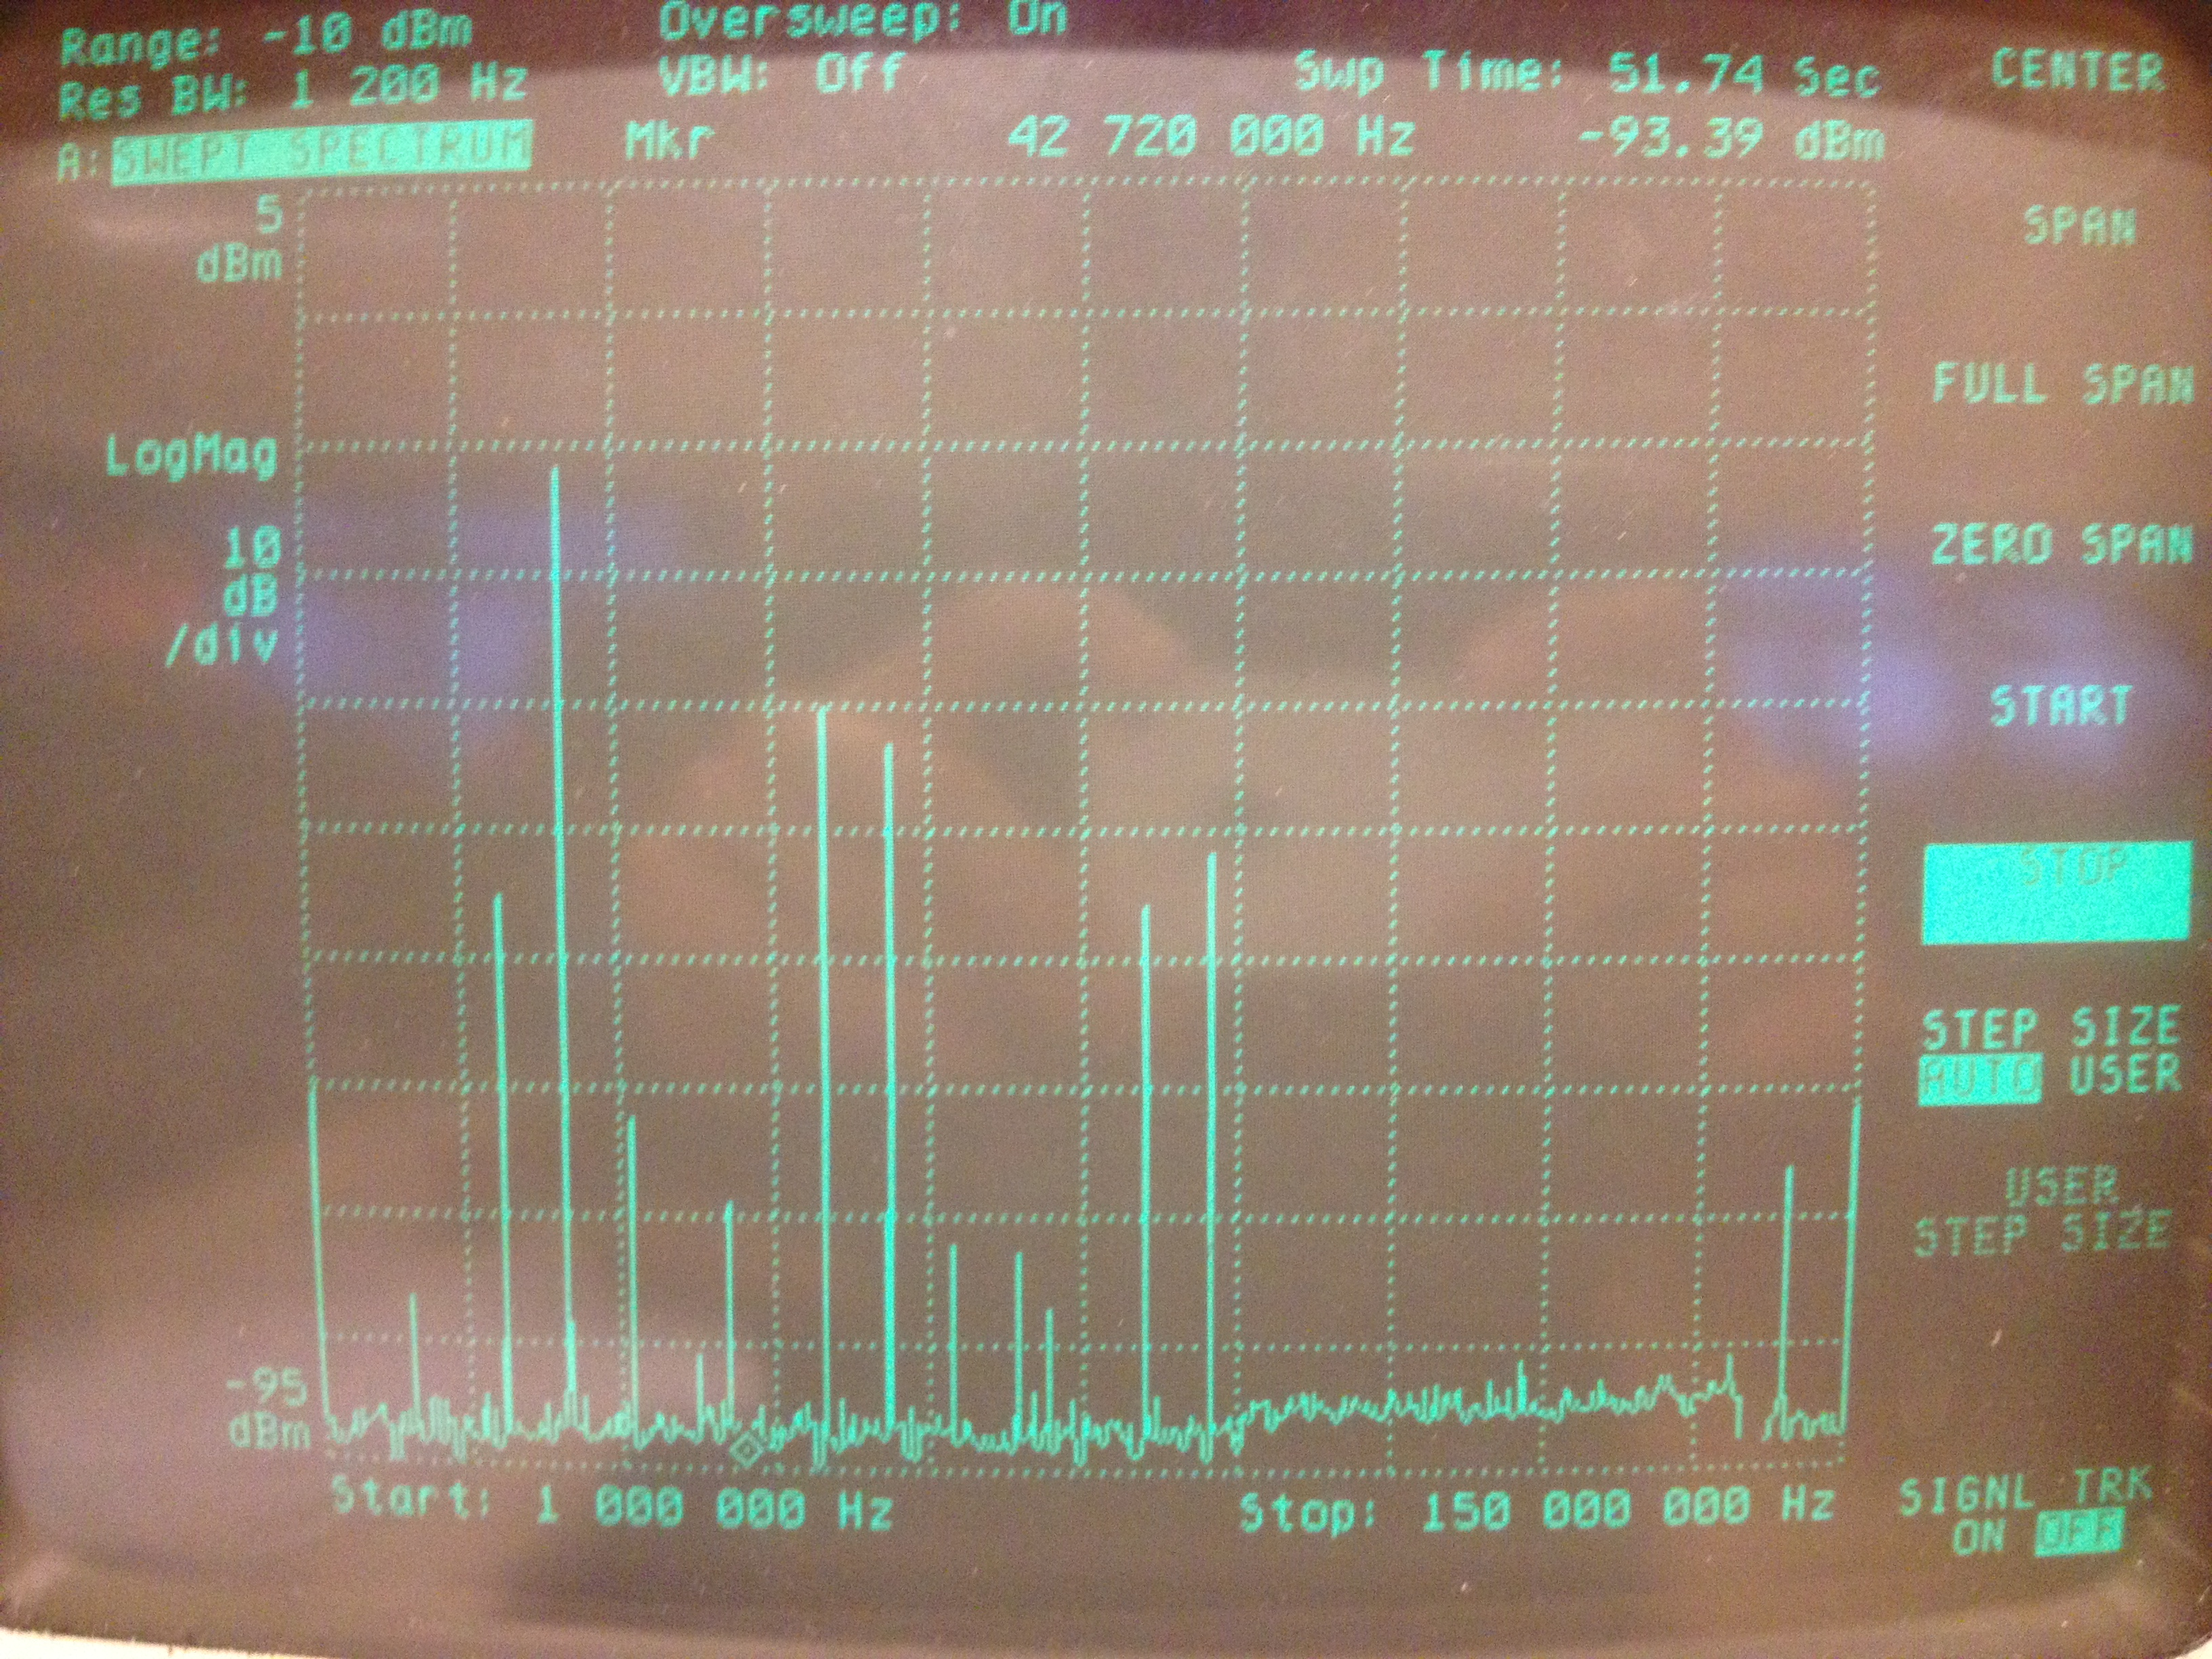
\includegraphics[width=.7\textwidth]{10_3_1}
	\caption{Réponse du mélangeur doublement équilibré à diodes de 1MHz à 150MHz}
	\label{fig:10_3_1}
\end{figure}

On constate qu'il y a nettement moins de raies qu'avec le mélangeur doublement équilibré, les harmoniques sont mieux atténuées.

\exsubpart{2}

On mesure, en zoomant autour des 14 MHz, une amplitude de sortie de -56.63dBm.
Il ne faut pas oublier de prendre en compte les étages d'adaptation d'impédance. L'adaptation en entrée réduit le signal de 6dB. Les résistance de 50$\Omega$ forment un pont diviseur de tension de facteur 0.5 qui se traduit par un gain de -6dB.
Alors que l'adaptation en sortie réduit le signal de 35.7dB (6dB à cause la résistance de 50$\Omega$ et 29.7dB à cause la résistance de 1.5k$\Omega$).

Le gain de conversion de G1 vers le drain est donc de : $-56.63+6+35.7-13.01= -27.94 dB$

\exsubpart{3}

On utilise la même démarche mise en œuvre pour les autres mélangeurs en augmentant progressivement la tension du signal RF d'entrée.
On trouve que le point de compression de 1 dB est à -3.4dBm.

\exsubpart{4}

On applique un signal 9MHz double ton, on cherche le taux de distorsion d'inter-modulation d'ordre trois.
En se plaçant à 10 dB en dessous du maximum pour notre signal d'entrée, on obtient le spectre suivant :

\begin{figure}[h!]
	\centering
	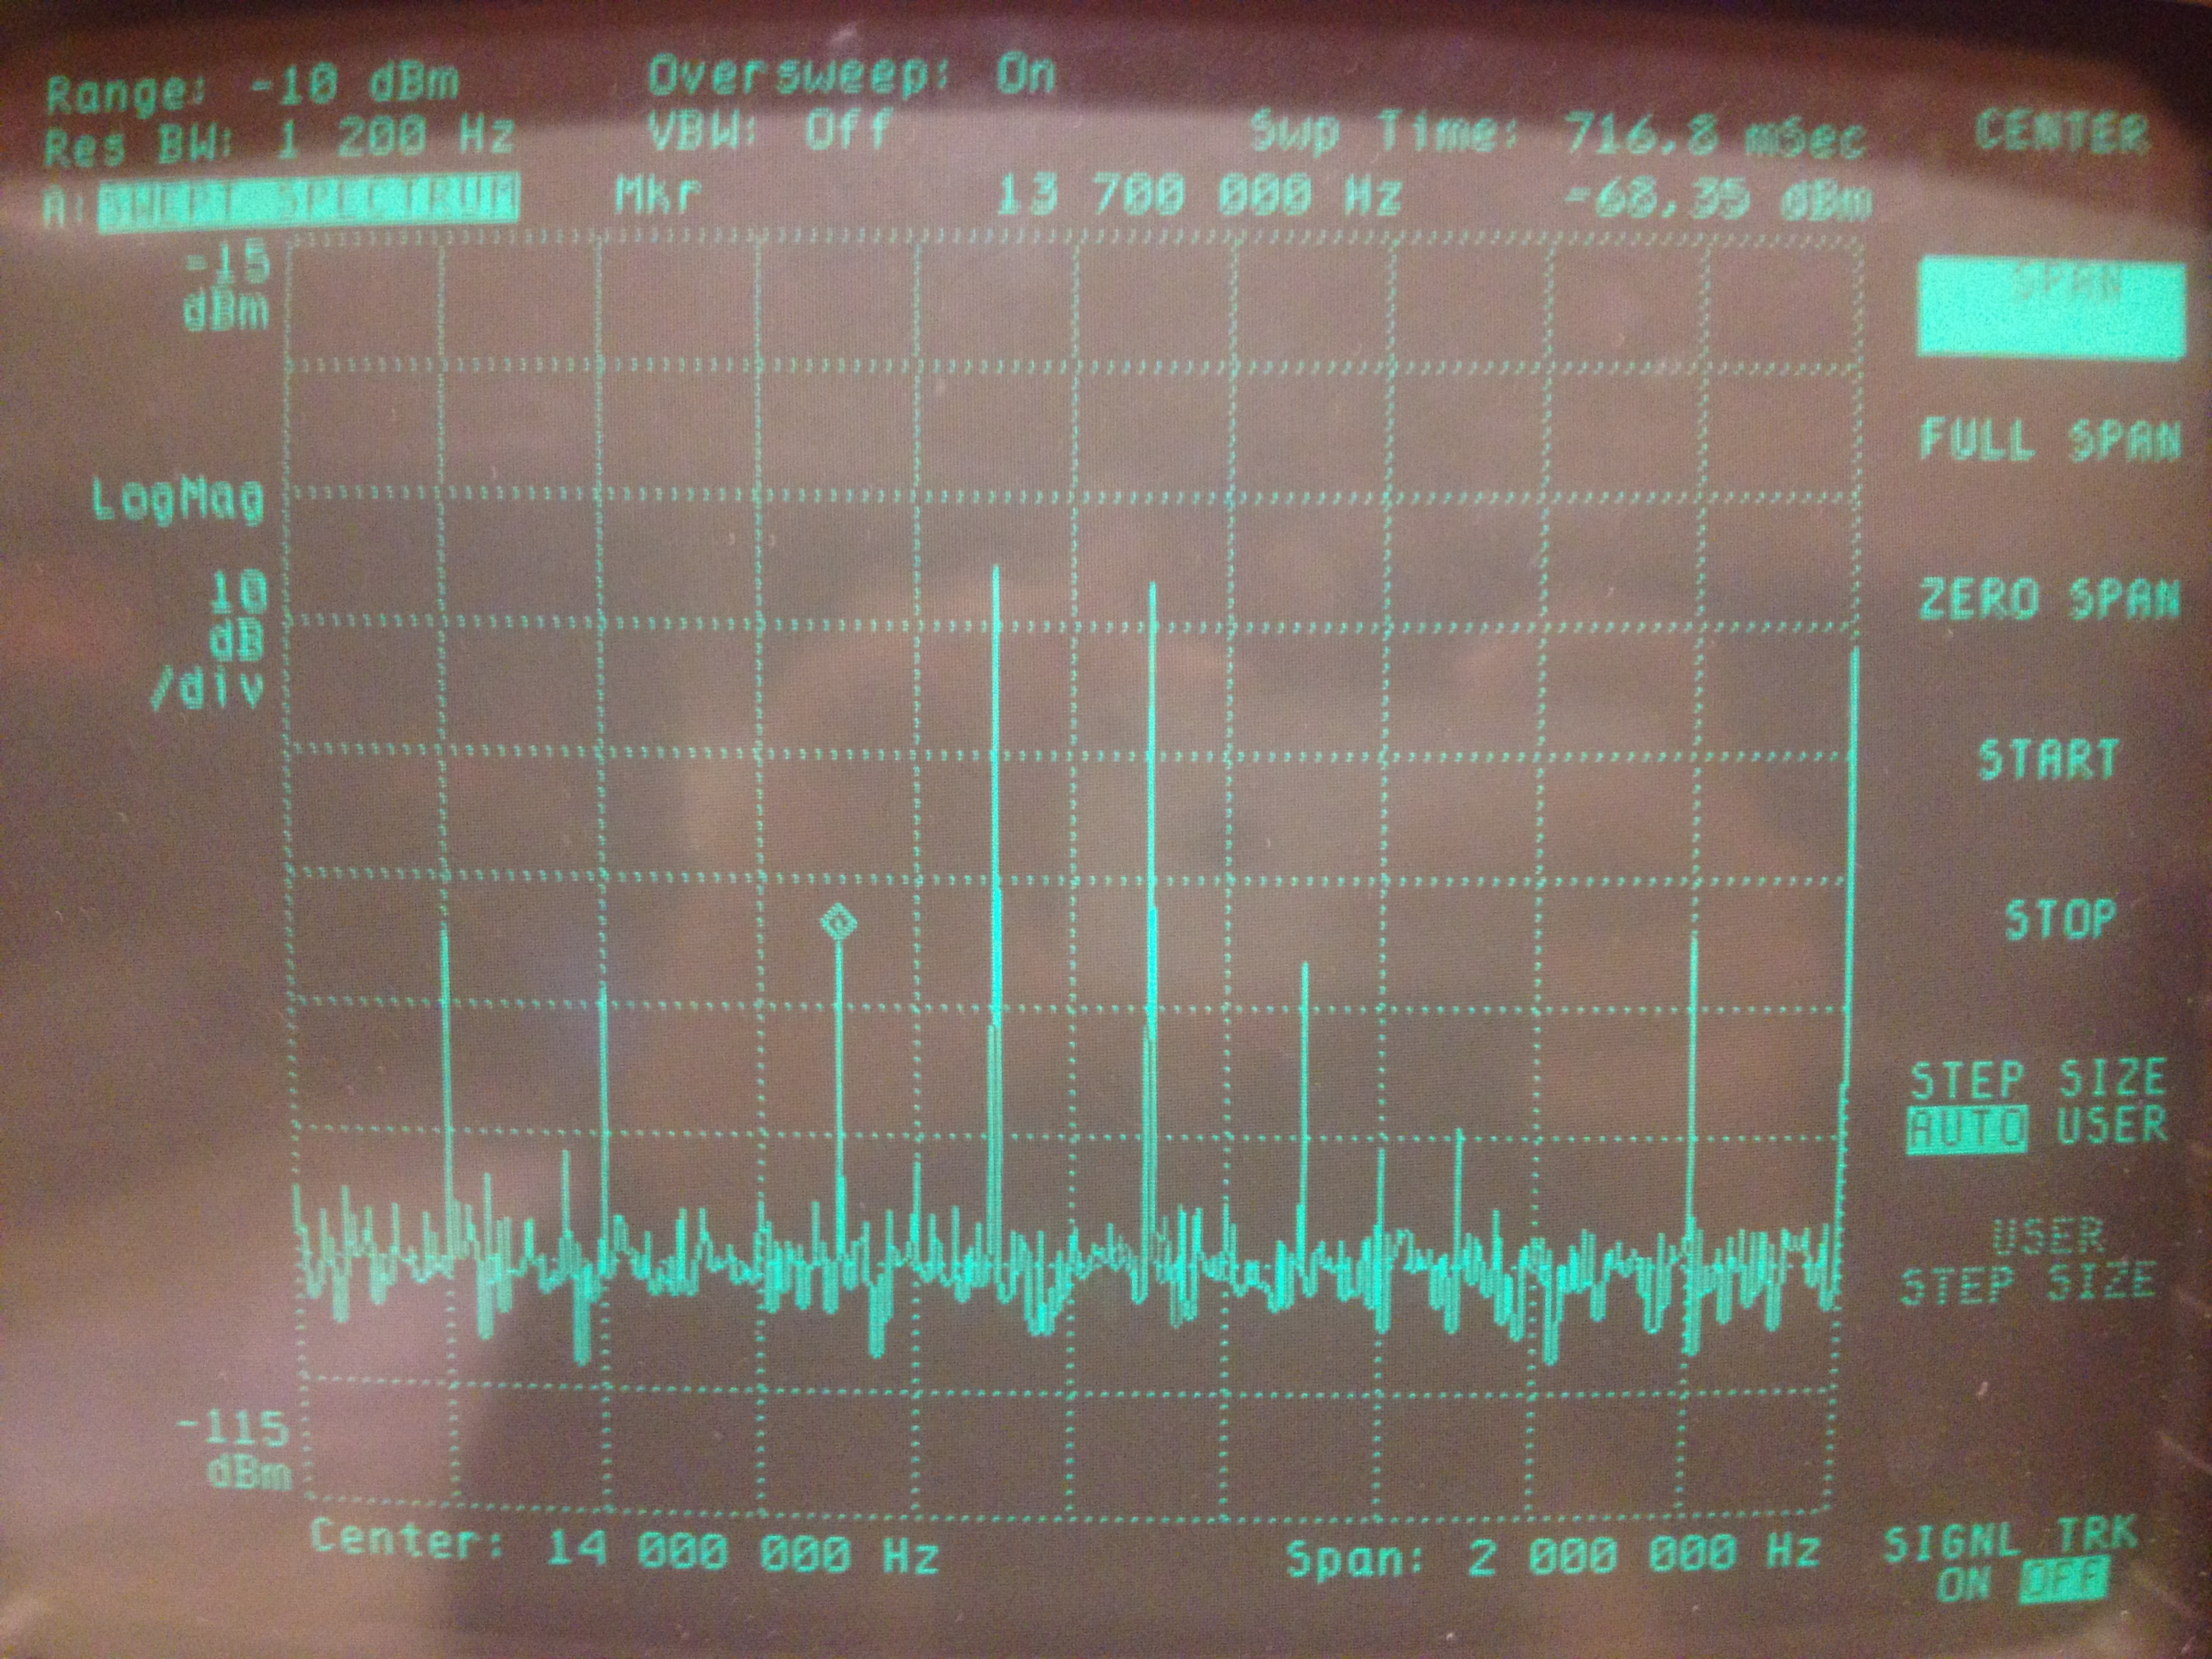
\includegraphics[width=.7\textwidth]{10_3_4}
	\caption{Spectre de la réponse à un signal double-ton à 8,9MHz et 9,1MHz}
	\label{fig:10_3_4}
\end{figure}

Le pic de l'harmonique de troisième ordre est de -5.4dBm soit 0.12Veff (après désadaptation).
%------------------------------------------------------------------------------------------------------------------
En appliquant la même formule que précédemment, on trouve OIP3=
%------------------------------------------------------------------------------------------------------------------


\exsubpart{5}

En chargeant la sortie avec une résistance de 50 ohms et observant à l'analyseur de spectre l'entrée IN2, on mesure un pic à 5MHz de -62.8dBm, ce qui correspond à un gain de conversion ou isolation  (insertion loss) ici de -75.8 dB.


\subsection{Le mélangeur à 1 diode}

On considère le mélangeur décrit Fig.~\ref{fig:schema_melangeur_diode}.
\begin{figure}[h!]
	\centering
	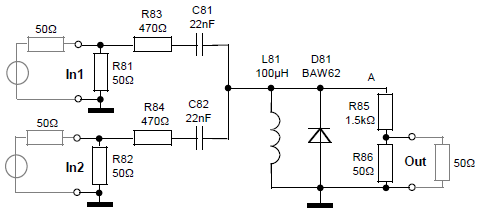
\includegraphics[width=.7\textwidth]{schema_melangeur_diode}
	\caption{Mélangeur à 1 diode}
	\label{fig:schema_melangeur_diode}
\end{figure}

Ce mélangeur à une diode est le montage le plus simple  et moins onéreux à réaliser parmi tous les mélangeurs étudiés. Mais ces avantages se paient par un spectre dense avec des harmoniques d'amplitude importantes.
Les deux signaux d'entrées IN1(RF) et IN2(LO) sont additionnés, on écrête ensuite le résultat grâce à la diode.
Ce dispositif est somme toute similaire à un dispositif « hacheur ».

\subsubsection{Questions et calculs}

\exsubpart{1}

$L_{81}$ permet de fixer la valeur moyenne ou valeur DC à 0 ce qui permet de faire conduire la diode correctement.

\exsubpart{2}

Les impédances réelles d'entrée et de sortie sont d'environ 50 $\Omega$, par analyse fréquentielle on trouve quelles sont comprises entre 45.19 et 48.79$\Omega$. Ce qui est environ 50$\Omega$.

Dans tous les cas, les 50$\Omega$ exacts sont difficilement atteignables en réalité à cause des tolérances des résistances et aux facteurs environnementaux.

\exsubpart{3}

Pour déterminer le courant maximum qui peut circuler dans In1 et In2, on applique la loi des nœuds en IN1 en considérant uniquement cette entrée.
On considère 2 cas :
%a refaire
\begin{itemize}
\item La diode est passante. Dans ce cas, le courant maximum qui revient sur l'une des entrées est égal à la moitié des courants entrants.

\item La diode est bloquante. Dans ce cas on a :
$I=i_{L}+i_{Out}+i_{dretour,max}$

On obtient après calcul :
$I=\frac{U_{out}}{R86}-j\frac{R86^2}{R86(R85+R86)L\omega}U_{out}+i_{dretour,max}$

\end{itemize}

\subsubsection{Mesures}

\exsubpart{1}

On applique sur IN2 (LO) une sinusoïde à 5MHz d'amplitude  2 Veff soit 19 dBm et sur IN1 (RF) une sinusoïde à 9MHz d'amplitude 10 mVeff soit -27 dBm.
On observe le signal de sortie entre 1 et 150MHz afin d'avoir une vue d'ensemble.

\begin{figure}[h!]
	\centering
	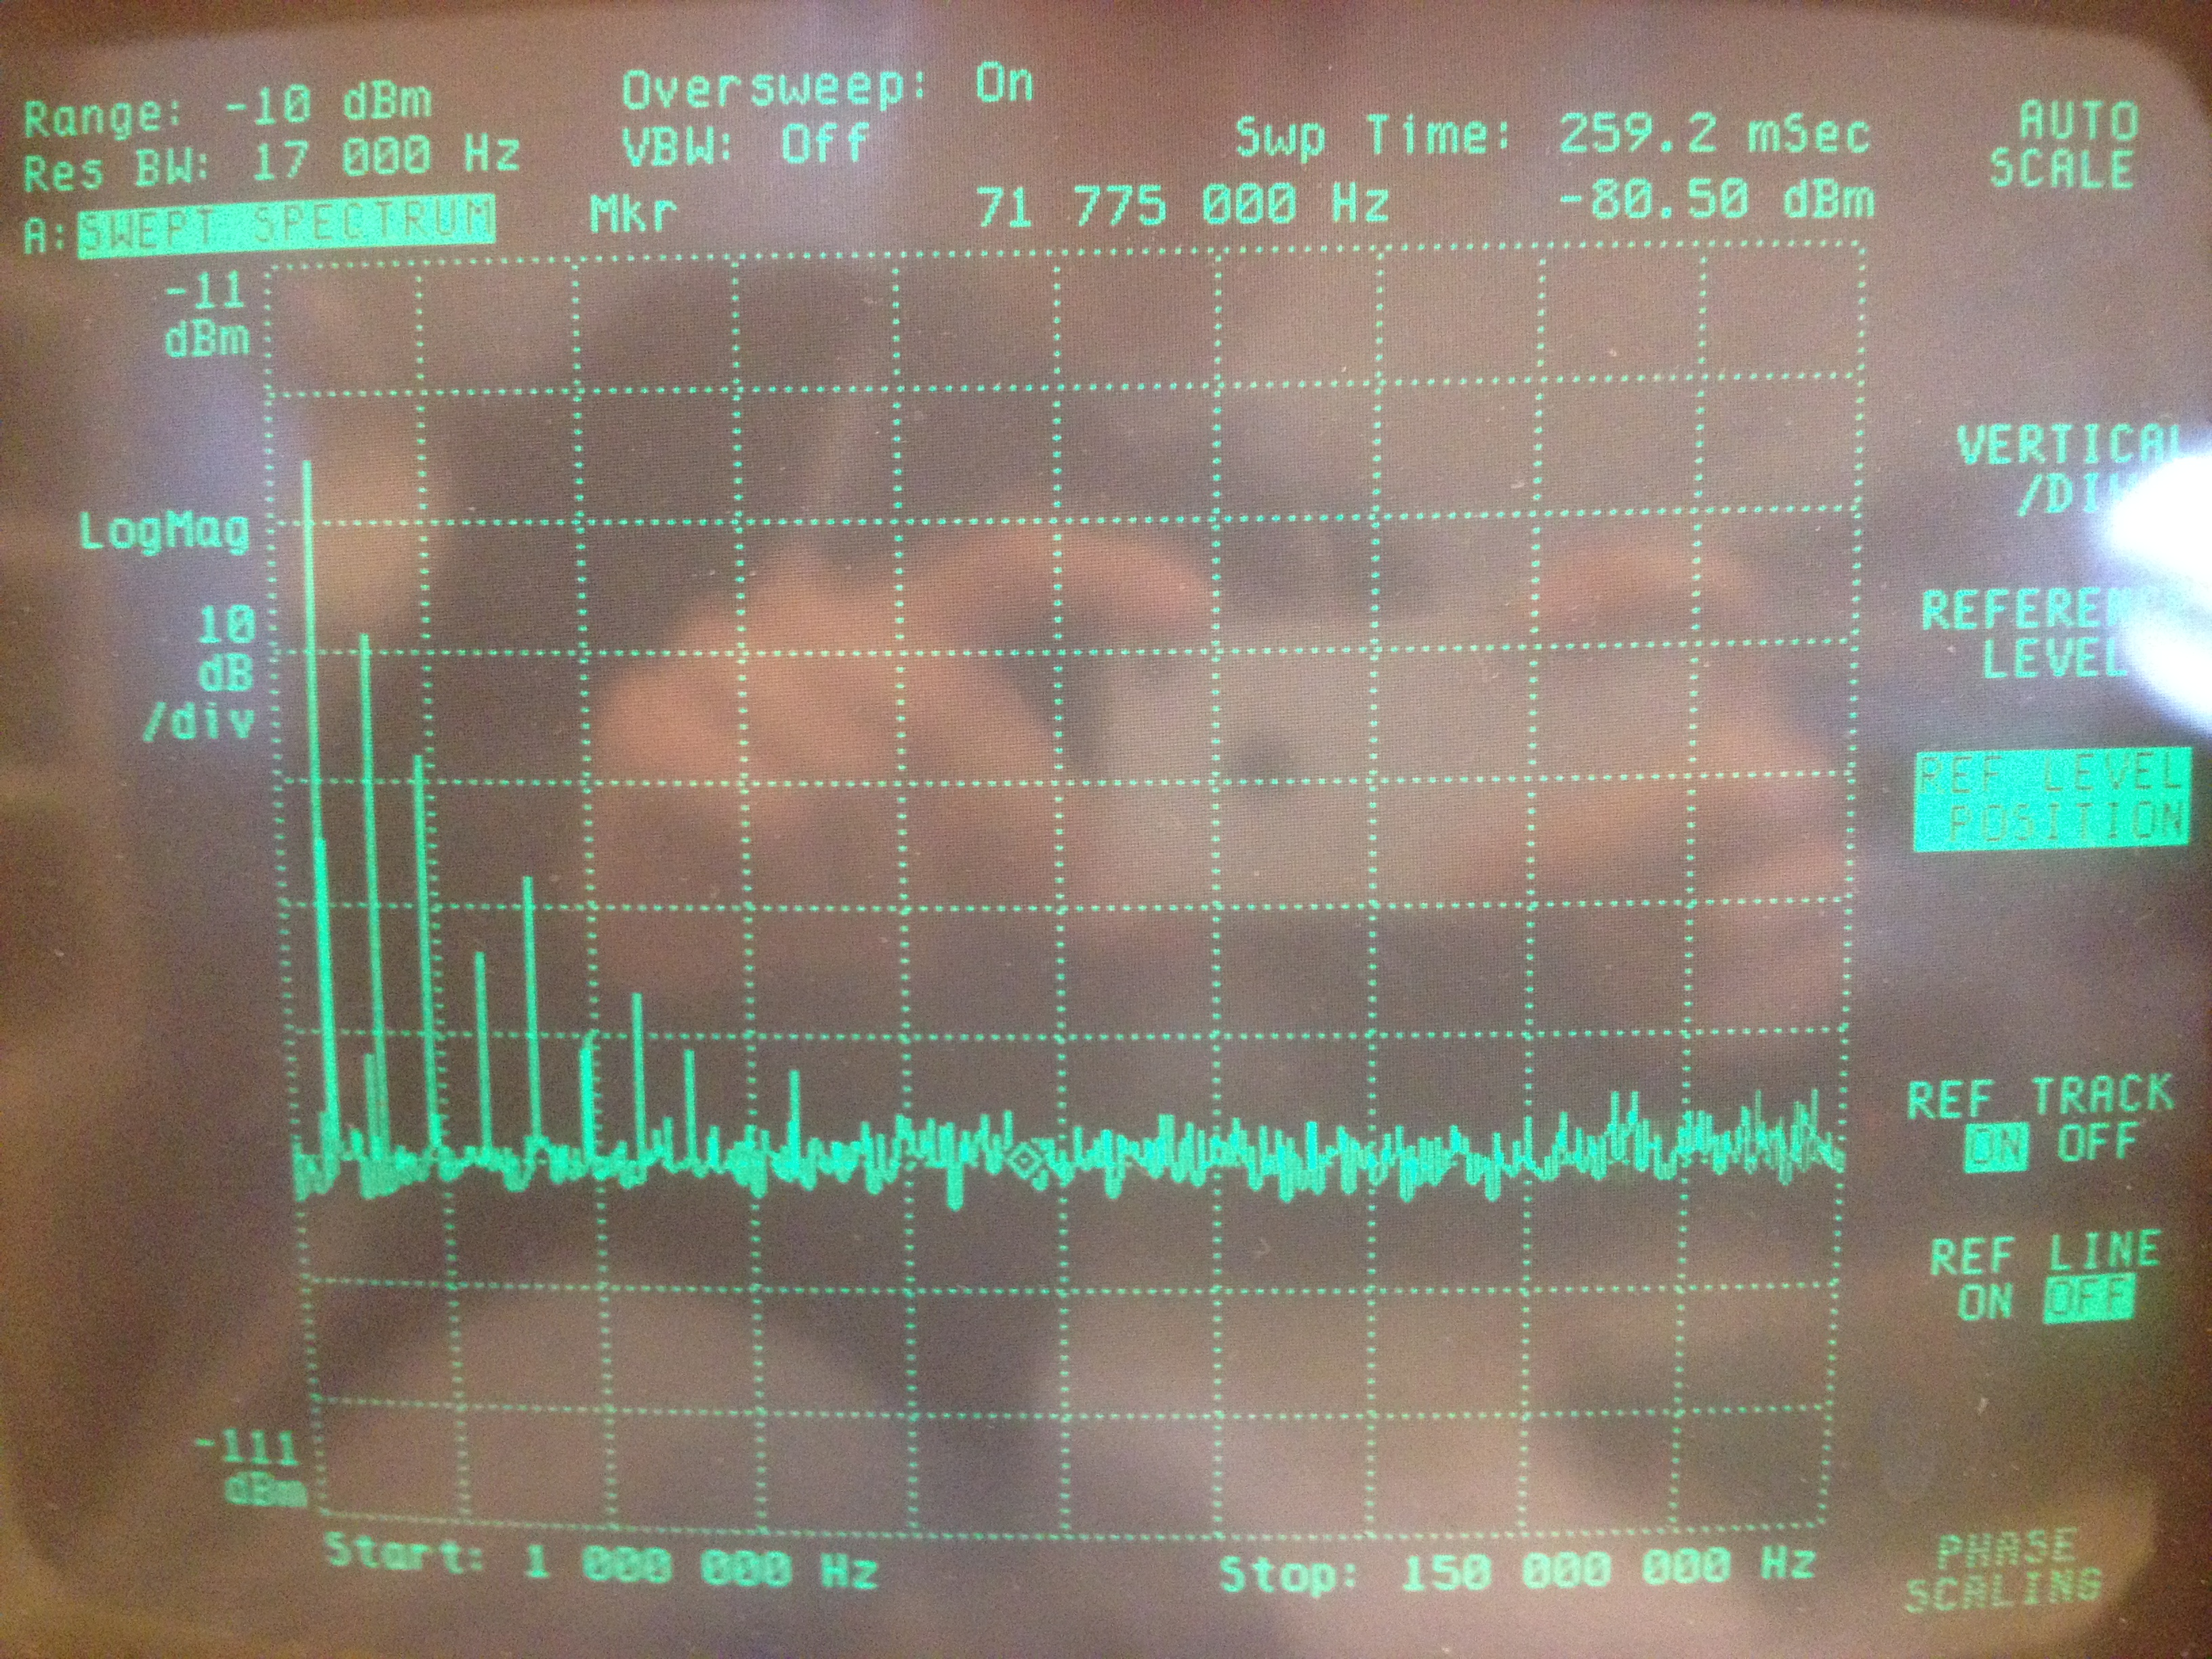
\includegraphics[width=.7\textwidth]{11_3_1}
	\caption{Réponse du mélangeur à 1 diode de 1MHz à 150MHz}
	\label{fig:11_3_1}
\end{figure}

Les harmoniques sont peu nombreuses mais d'amplitude conséquentes ! Tous les signaux supérieurs à environ 50MHz sont filtrés grâce à on sait pas.
%à éclaircir ou pas

\exsubpart{2}
On mesure, en zoomant autour des 14 MHz, une amplitude de sortie de -80.1dBm.

Le gain étant très faible, nous avons été obligé d'augmenter légèrement l'amplitude d'entrée de In1 à 20 mVeff soit -21 dBm en constatant qu'à partir d'un certain niveau, le gain restait constant. La mesure réalisée est un peu moins atténuée et sujette au bruit et donc plus précise.

L'amplitude de sortie est alors de -75dBm.
En prenant en compte les étages d'adaptation d'impédance, le gain de conversion est de 12.3 dB.

\exsubpart{3}

On utilise la même démarche mise en œuvre pour les autres mélangeurs en augmentant progressivement la tension du signal RF d'entrée.
%Pour une amplitude d'entrée de 18.5dBm, la sortie à 14MHz a une amplitude de -36.6dBm, ce qui correspond à un gain de  %conversion de +23.6 dB.
%
%FAUX?
On trouve que le point de compression de 1 dB est à 18.5dBm.

\exsubpart{4}
On applique un signal 9MHz double ton, on cherche le taux de distorsion d'inter-modulation d'ordre trois.
En se plaçant à 10 dB en dessous du maximum pour notre signal d'entrée, on obtient le spectre suivant :

\begin{figure}[h!]
	\centering
	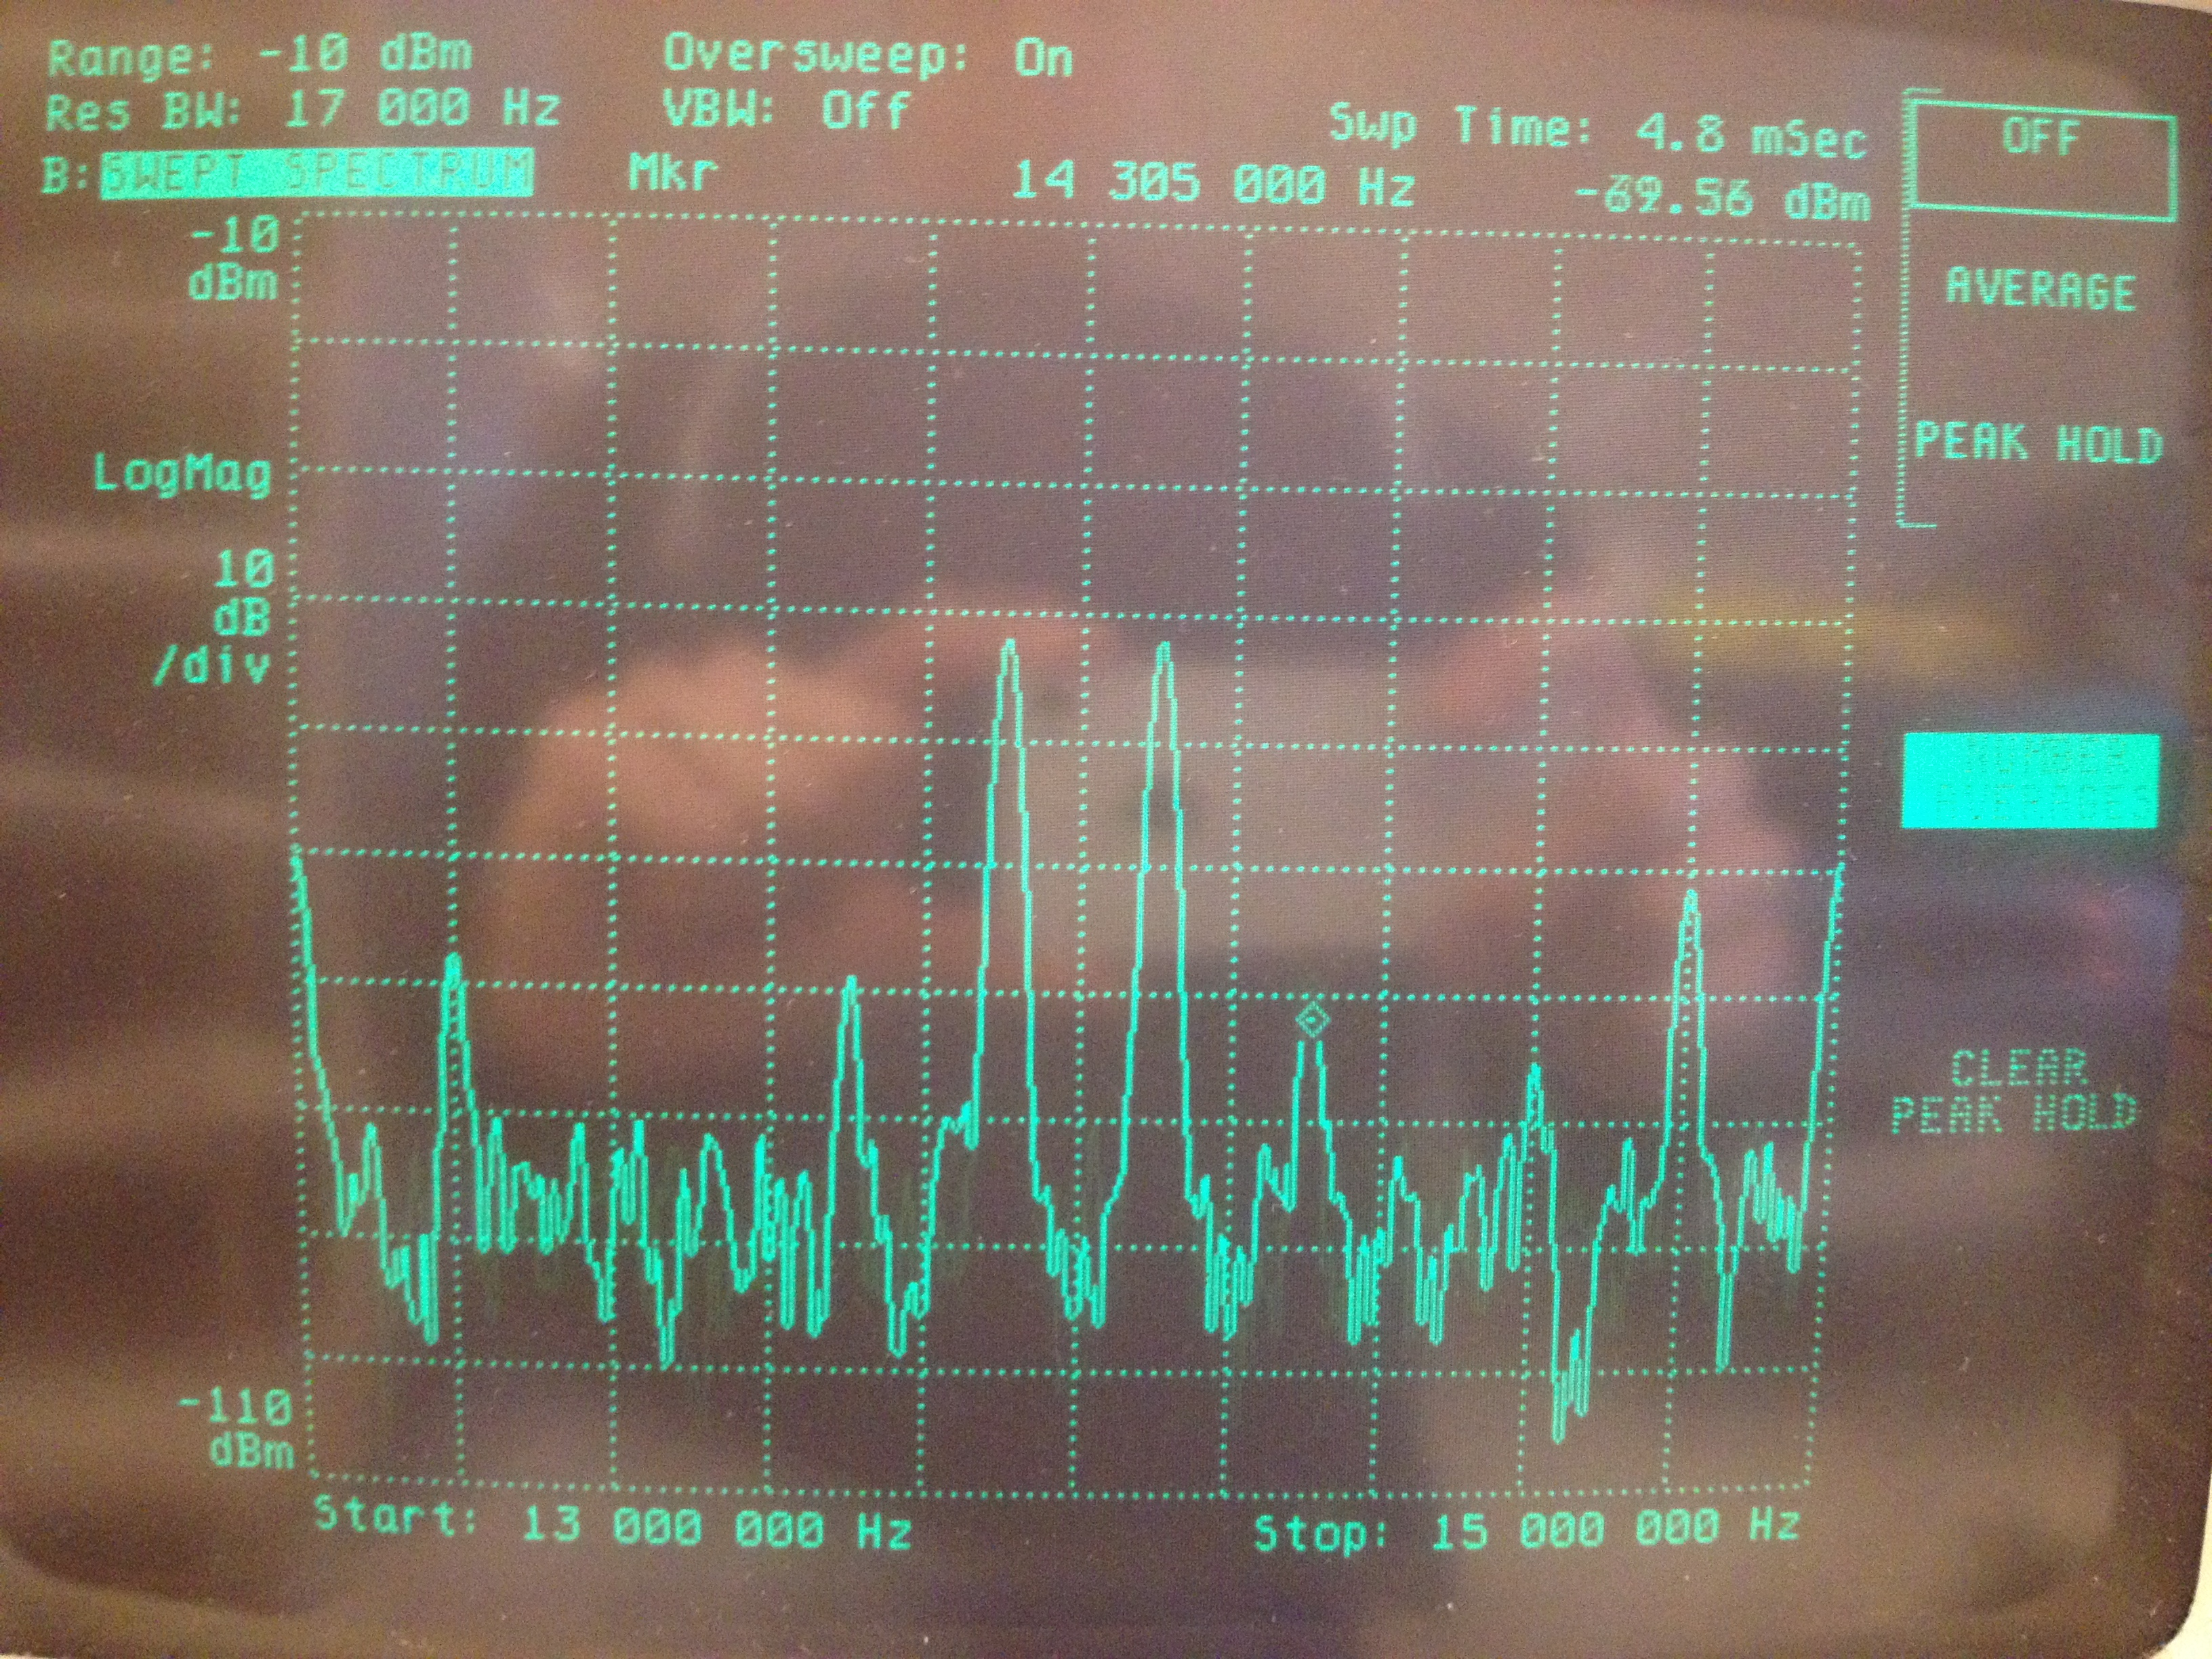
\includegraphics[width=.7\textwidth]{11_3_4(2eme_point)}
	\caption{Spectre de la réponse à un signal double-ton à 8,9MHz et 9,1MHz}
	\label{fig:11_3_4}
\end{figure}

Le pic de l'harmonique de troisième ordre est de -70.2dBm.
%------------------------------------------------------------------------------------------------------------------
En appliquant la même formule que précédemment, on trouve OIP3=
%------------------------------------------------------------------------------------------------------------------


\exsubpart{5}
En chargeant la sortie avec une résistance de 50 ohms et observant à l'analyseur de spectre l'entrée IN2, on mesure un pic à 5MHz de -16.48dBm, ce qui correspond à un gain de conversion ou isolation  (insertion loss) ici de -35.48 dB.

\begin{figure}[h!]
	\centering
	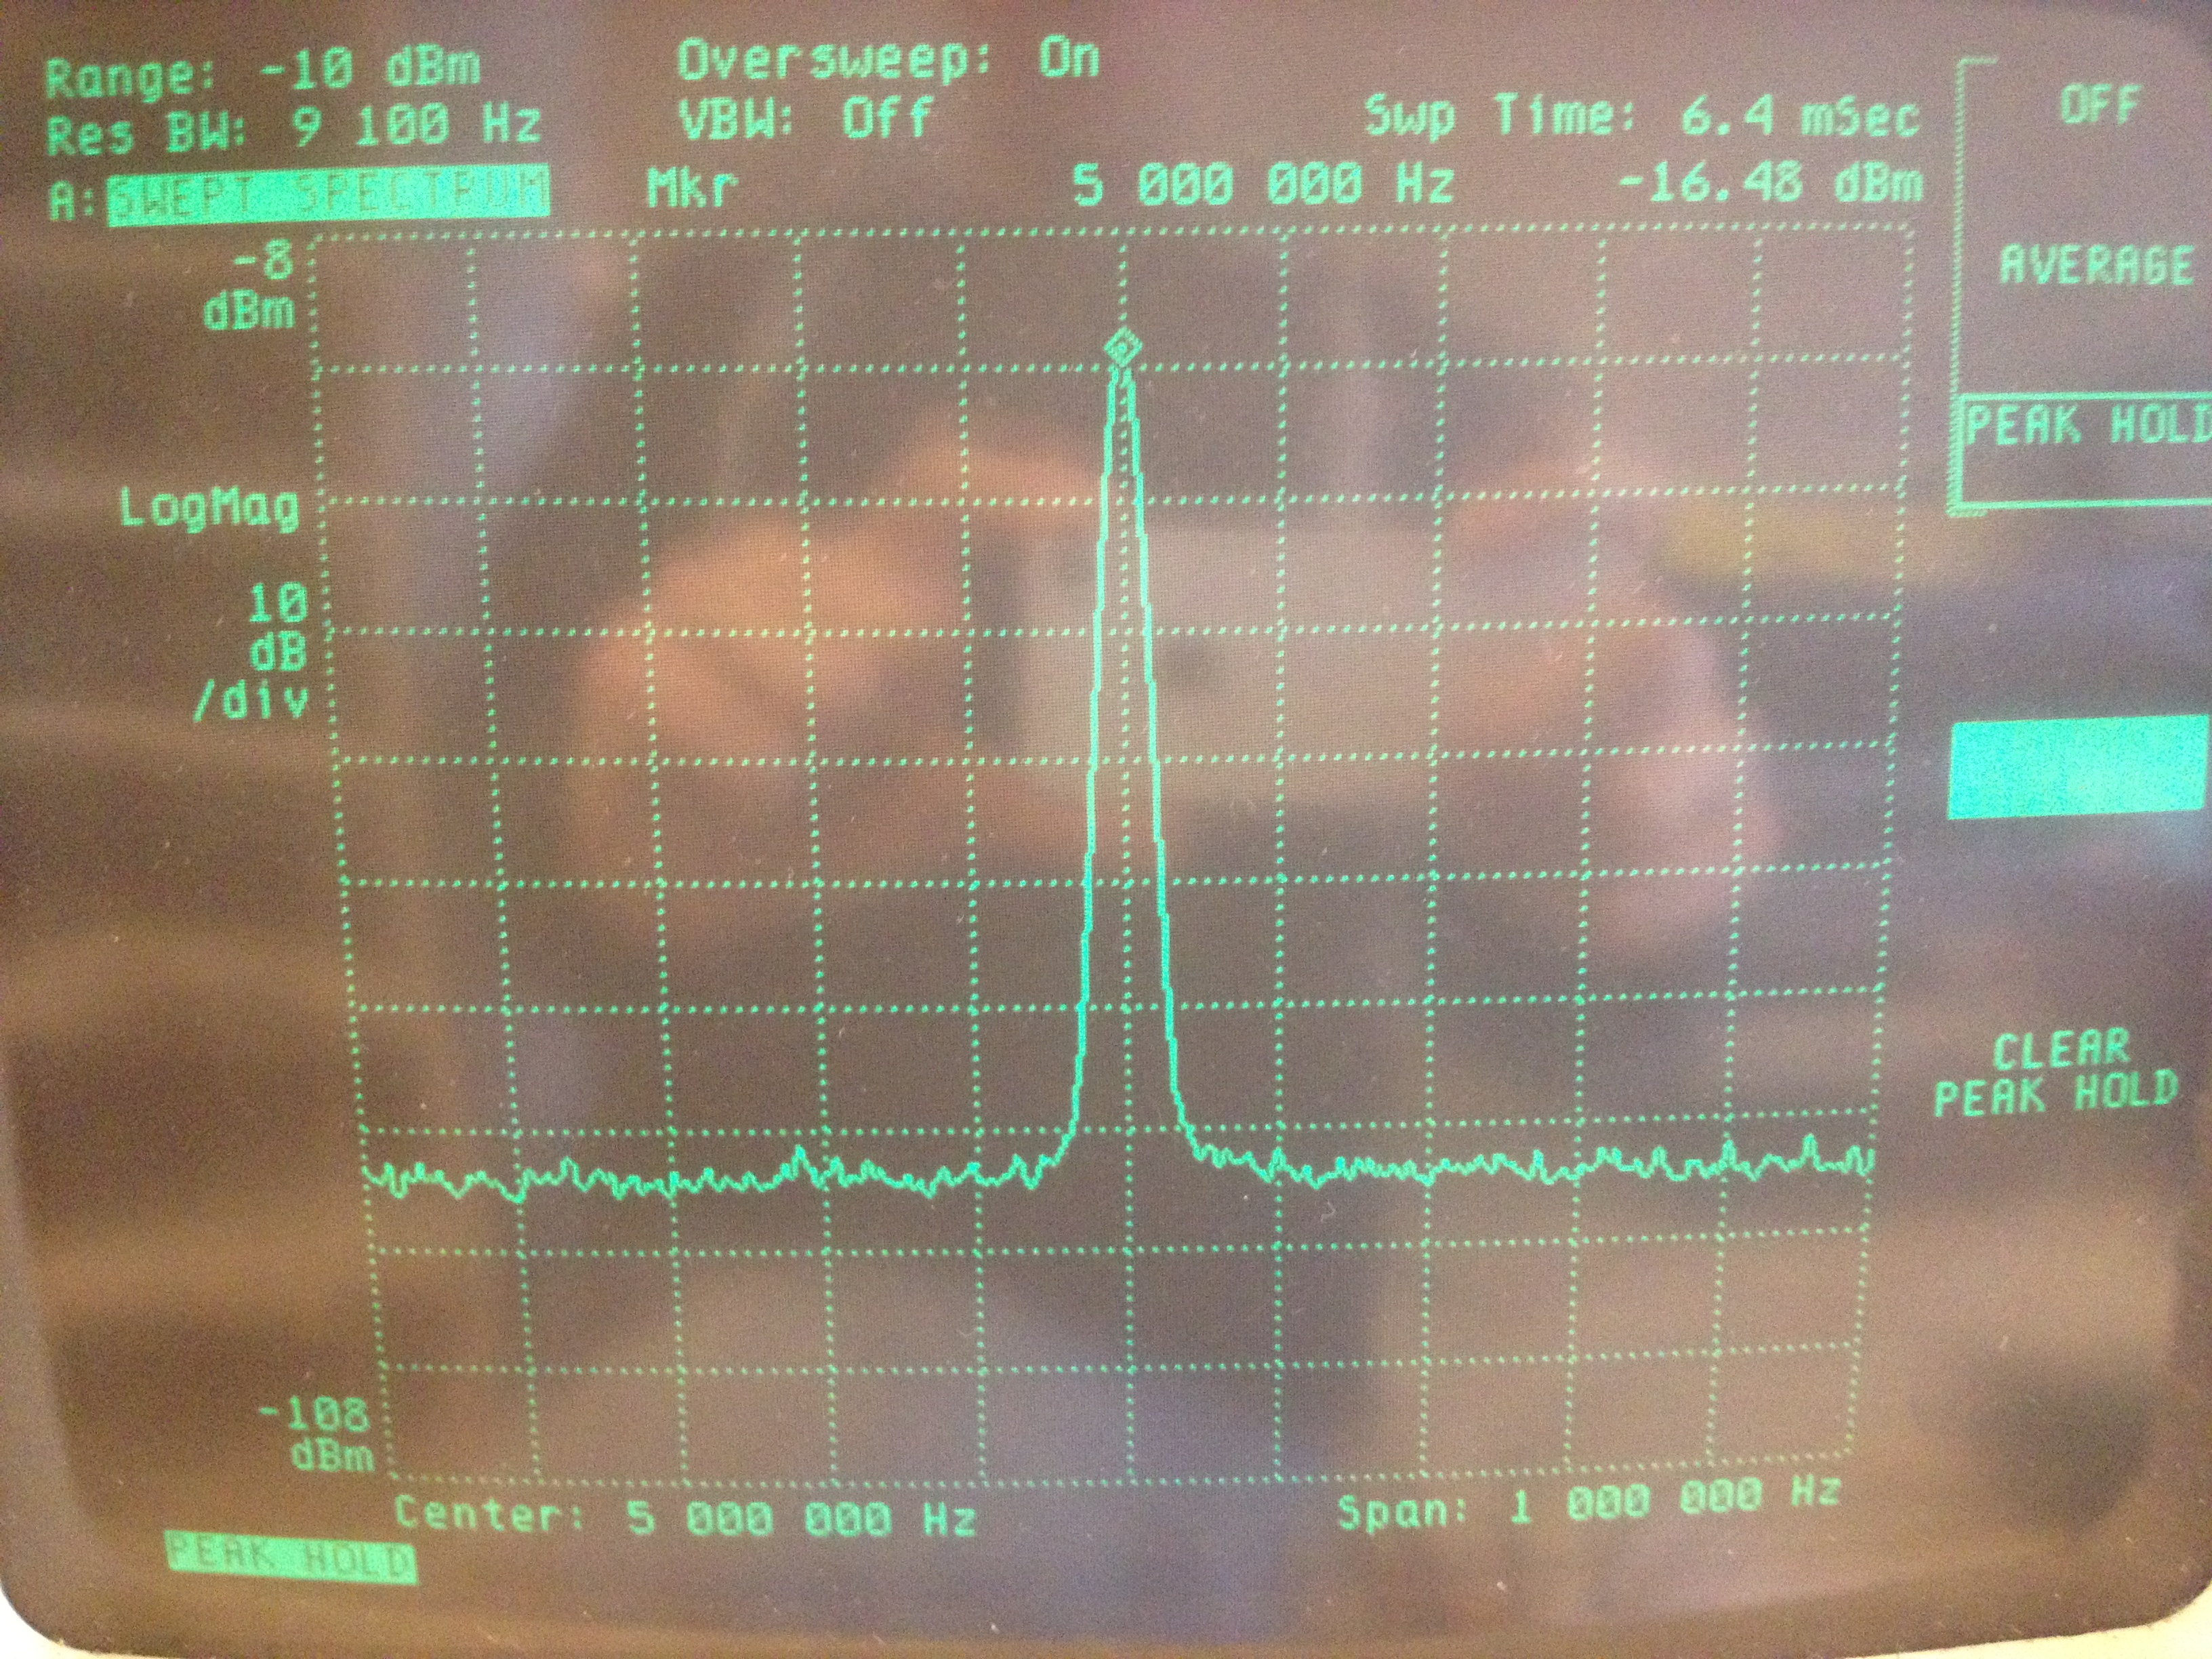
\includegraphics[width=.7\textwidth]{11_3_5}
	\caption{Isolation de l'entrée IN2 vers IN1}
	\label{fig:11_3_5}
\end{figure}

\subsection{Conclusions sur les mélangeurs}

\exsubpart{1}

Tableau récapitulatif des trois types de mélangeurs analysés:

\begin{tabular}{|c|c|c|c|c|c|}
\hline Gain de conversion& Pertes d'insertion& Spectre& Simplicité et coût& Alimentation& Autres \\
\hline Mélangeur doublement équilibré à diodes & & & & Passif& a \\ 
\hline Mélangeur à « MOS double-gate » &  & & & Actif 7V& a  \\ 
\hline Mélangeur à 1 diode &  & & & Passif& a  \\ 
\hline 
\end{tabular} 


\exsubpart{2}

Chaque type de mélangeurs est exploité pour ses qualités respectives. On retrouve ainsi leurs usages dans différents domaines de l'industrie.
\begin{itemize}

\item Le mélangeur doublement équilibré est par exemple utilisé comme tête de réception pour la télévision satellite analogique avec une bi-bande allant de 10,8 à 11,8 GHz et de 11,8 à 12,8 GHz.
Il est aussi utilisé dans les récepteur de télécommande (Modulation AM).
\item Le mélangeur à « MOS double-gate » est utilisé comme récepteur TV VHF.
\item Le mélangeur à 1 diode est quant à lui utilisé dans les radars Doppler Hyperfréquence. On mélange le signal reçu à la fréquence f’(renvoyée par l'objet) au signal émis f par la diode, le signal produit possède une fréquence différence liée à la vitesse v de l'objet. 
\end{itemize}

% Est-ce vraiment correct ? Normalement on devrait être à -18 dBm (10 dB en dessous du point de compression, PAS à -8 dBm ?

%  9
%
%  In 9MHz = +7 dBm
%  In 5MHz = -7 dBm
%  Pic en sortie à 14MHz = -12.5 dBm
%  => Gain de conversion = -5.5 dB
%
%  In 5Mhz = 1 dBm  =>  Pic sortie 14MHz = -5.5 dBm, soit gain = -6.5 dBm
%  => Point de compression : In RF à 1dBm, soit 0.250 Veff
%
%  In1: 9MHz = 7 dBm
%  Out: 50.47 Ohm
%  In2: analyseur de spectre  =>  -58.5 dBm
%  =>  Gain = -67.5 dB
%


% 10
%
% On prend R77 = 560, R76 = 3.3k (on veut R76/R77=6)
% L72 pour fixer à 0 le potentiel moyen à G1 (sinon, on ne contrôle pas ce potentiel moyen). Comme ça, on peut polariser négativement blablabla G1.
%
% LO : 5MHz, 1Veff, 13.01 dBm
% RF : 9MHz, 10mVeff, -27dBm
% Sortie : plein d'harmoniques : multiples de 5MHz, de 9MHz, 9-k5 ...
% 14 MHz : -56.63 dBm
% Gain : -30.37 dB avec les réductions en entrée (Rin, R72) (-6dB) et en sortie (R73,R74,Rout) (-35.7 dB)
%    soit, sans ces adaptations : 11.33 dB
% Compression 1dB : In à -3.4 dBm, soit 0.151 Veff
%
% In2 : 5 MHz, 1 Veff
% IN1 : 9.1 MHz, 8.9 MHz, -5.4 dBm, 0.12 Veff
% => 14.3 MHz (3e harmo mesurée) : -70.9 dBm
%   (14.1 MHz : -42dBm)
%
% Avec 50.47ohm en sortie, IN2 avec 1Veff (13.01 dBm), l'analyseur sur IN1 :
% on mesure à 5MHz : -62.8 dBm
%  => -75.8 dB


% 11
%
% In1 : 10 mVeff, 9 MHz, -27 dBm
% In2 :  2 Veff,  5 Mhz, 19 dBm
% Sortie 14MHz : -80.1 dBm
% Gain : -53.1 dBm
% En prenant en compte les diviseurs de tensions internes : -11.4 dBm
% On réalise qu'en augmentant légèrement In1 à partir de 10mVeff, le gain augmente légèrement,
% avant de devenir constant pour une large gamme d'amplitudes pour In1.
% On fait donc les mesures de gain pour une amplitude de In1 légèrement supérieure à 10 mVeff :
% 20 mVeff
%
% in1 : 20 mVeff, -21 dBm
% Sortie 14MHz : -75 dbm
% Gain : -54 dBm
% En prenant en compte les diviseurs de tensions internes : -11.4 dBm
%
% In1 : 18.5 dBm  =>  Sortie 14MHz : -36.6 dBm
% = Gain de compression à -1dB
%
% In1 13.9 MHz, 14.1 MHz : 1.88 Veff, 18.5 dBM
% Sortie 14.3 MHz : -70.2 dBm
%

\end{document}